\documentclass[E5,LUFonts]{lundphdthesis}
% Note using overleaf: Compile with "XeLaTeX" if you want LU fonts

% Possible options:
% E5 or G5 depending on size of thesis book
% LUFonts for using LU chosen fonts
% MathFonts for using the LU chosen fonts for math mode, I don't really think it looks good

\newcommand\scalemath[2]{\scalebox{#1}{\mbox{\ensuremath{\displaystyle #2}}}}
\newcommand{\longunderbrace}[2]{\underbrace{#1}_{\text{\hbox to 0cm{\hss #2 \hss}}}} 
% ==================================
% ==================================
% ==================================
%
% FRONTMATTER
%
% ==================================
% ==================================
% ==================================

\title{Stellar kinematics in surveys and simulations}
%\subtitle{subtitle here}   % optional
\author{Daniel Mikkola}

\degree{Thesis for the degree of Doctor of Philosophy}
\titleblurb{Thesis advisor: Dr.\ David Hobbs\\
Co-advisor: Dr.\ Paul McMillan\\
Faculty opponent: Dr.\ Marie Martig}
\announcement{To be presented, with the permission of the Faculty of Science of Lund University, for public criticism in the Lundmark lecture hall (Lundmarksalen) at the Department of Astronomy and Theoretical Physics on the ${18}^\textrm{\tiny th}$ November 2022 at 13:00.}

\begin{document}

\maketitleshort   %this one is optional


% ==================================
% "spikningsblad" consists of title with blurb and a data sheet paper
% if the entire spikningsblad is in pdf format these two pages can be handled with includepdf
\maketitlewithblurb
\newpage

% the following overlay the total page number count dynamically, adjust vspace and hspace accordingly
% if too many problems with that, just use \includepdf{datasheet_name} instead
%\includepdf{datasheet_name}
\AddToShipoutPictureBG*{\AtPageLowerLeft{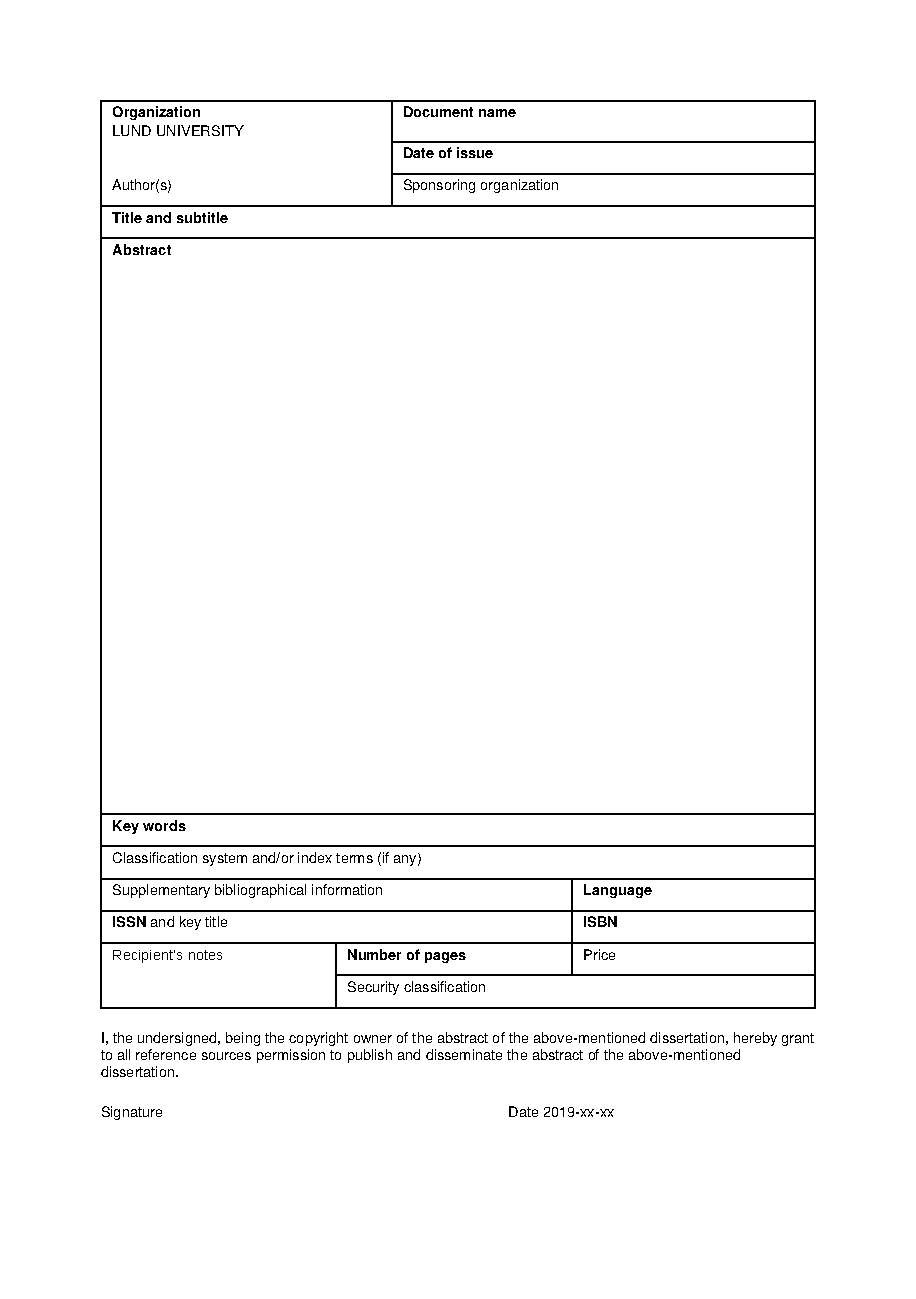
\includegraphics[width=\paperwidth,height=\paperheight]{datasheet_empty.pdf}}}
\vspace*{13.75cm}\hspace*{6.1cm}{\footnotesize\ztotpages}   % modify the distances and font size as needed
\newpage


% ==================================
% actual title page
\maketitle


% ==================================
% make page with evaluation committee and copyright information
\newpage
\begin{center}
	\textbf{Faculty Opponent} \\
	\vspace{1em}
	Dr.\ Marie Martig\\
	Astrophysics Research Institute, Liverpool John Moores University,\\
	Town, Country\\
	\vspace{1.5em}
	\textbf{Evaluation Committee} \\
	\vspace{1em}
    Dr.\ Someone Someoneson\\
    Department of Astronomy, Someplace University,\\
    Town, Country\\
    \vspace{0.7em}
    Dr.\ Someone Someoneson\\
    Department of Astronomy, Someplace University,\\
    Town, Country\\
	\vspace{0.7em}
    Dr.\ Someone Someoneson\\
    Department of Astronomy, Someplace University,\\
    Town, Country\\
\end{center}
\vfill

{\small\parindent0pt
\textbf{Front cover:} Explanation of the front cover.
Credit: xx Edited by xx and printed with permission from xx.

\textbf{Back cover:} .

\textbf{Funding information:} This thesis work is financially supported by -.

\vspace{1em}
\copyright\, Daniel Mikkola 2022

\vspace{1em}
Faculty of Science, Department of Astronomy and Theoretical Physics

\vspace{1em}
ISBN: ~(print)\\ % ISBN av svenska ISBN centralen
ISBN: ~(pdf) % ISBN av svenska ISBN centralen

\vspace{1em}
Printed in Sweden by Media-Tryck, Lund~University, Lund 2022\\

\includegraphics[width=0.5\textwidth]{logo/miljoeloggor}
}

% ==================================
% dedication page
\newpage

\vspace*{140pt}
\begin{flushright}
\textit{Till morfar}
\end{flushright}

% ==================================
% table of contents
\cleardoublepage
\frontmatter
\pagestyle{plain}
\setcounter{page}{1} % Page Roman 1 of the frontmatter
\setcounter{tocdepth}{1}
\setcounter{secnumdepth}{2}
\renewcommand{\thesection}{\arabic{chapter}.\arabic{section}}
\tableofcontents


% ==================================
% Work list and popular abstract
\newpage
\sectionhidenum{List of publications}

This thesis is based on the following peer-reviewed publications:
\vspace{1mm}

% \phdarticle{title}{authors}{journal}
\phdarticle{Radial migration and vertical action in N-body simulations}
{\textbf{Mikkola, D.}; McMillan, P. J.; Hobbs, D. (2020)}
{Monthly Notices of the Royal Astronomical Society, Volume 495, Issue 3, pp. 3295-3306}
\phdarticle{The velocity distribution of white dwarfs in Gaia EDR3}
{\textbf{Mikkola, D.}; McMillan, P. J.; Hobbs, D.; Wimarsson, J (2022)}
{Monthly Notices of the Royal Astronomical Society, Volume 512, Issue 4, pp. 6201-6216}
\phdarticle{The velocity distribution of local halo and disk stars in Gaia DR3 from transverse motion}
{\textbf{Mikkola, D.}; McMillan, P. J.; Hobbs, D. (2022)}
{\textit{Submitted to Monthly Notices of the Royal Astronomical Society}}%Monthly Notices of the Royal Astronomical Society, Volume VVV, Issue I, pp. pppp-pppp}
%\phdarticle{Paper 4 title}
%{\textbf{Mikkola, D.}; McMillan, P. J.; Hobbs, D. (2020)}
%{Monthly Notices of the Royal Astronomical Society, Volume VVV, Issue I, pp. pppp-pppp}
%\phdarticle{nishiyama stars ...}
%{\textbf{Thorsbro, B.}; Ryde, N.; Rich, R. M.; ...}
%{In manuscript}
\makephdarticletable


\noindent Papers I, II, and III  are reproduced with permission from Monthly Notices of the Royal Astronomical Society.

\newpage

%\newpage
%\noindent Positions of trust undertaken during the PhD education:
%\begin{enumerate}
%    \item Secretary of the PhD student union at the Faculty of Science, 2017/18.
%    \item Chair of the PhD student union at the Faculty of Science, 2018/19, representing approximately 450 PhD students.
%    \item Chair of the PhD student union at Lund University, 2019/20, representing approximately 2100 PhD students.
%\end{enumerate}

%\vspace{2mm}
%\begin{center}
%\begin{minipage}{0.7\linewidth}
%\textit{``An easily governed university is no university at all.''}
%
%~\hfill\footnotesize{\citep{boultonlucas:08}}  %(Boulton and Lucas, 2008)
%\end{minipage}
%\end{center}


% ==================================
% Popular summary (ENGLISH)
\sectionhidenum{Popular summary}
Of all things on the celestial vault the greatest and most striking is the diffuse band of stars that make up the Milky Way, our home Galaxy. To understand how it formed and evolved we need, among other things, a detailed description of how the stars move and where they are located, the field of research called \textit{astrometry}. The first stellar catalogue was created 200 BCE by Hipparchus in ancient Greece. A little over two millennia later we began measuring stars with space telescopes, the first of which was named \textit{Hipparcos}. This was succeeded by the space telescope \textit{Gaia} which was launched in 2013 and revolutionized the field of astrometry, providing a truly great catalogue of stellar motions and positions. This catalogue has significantly contributed to the research behind this thesis. \textit{Gaia} gives us a very precise picture of how the Milky Way kinematics look today. To complete the picture one also uses numerical simulations to recreate and interpret the features found in observations. The union of theory and observations then reinforce one another and is critical for our understanding of the Milky Way.

The first article in this thesis uses numerical simulations to study how interactions with the Galaxy's spiral arms and bar transports stars radially in the plane of the disc. We find that this migration depends on the Galactic disc's strength and how vertical extended the stellar orbit is. With over 100 simulated discs we could determine that in less massive discs it is mostly the stars close to the disc that migrate and in the opposite case of massive discs they migrate regardless of how far above the disc the orbit goes.

In the second and third articles we use data from \textit{Gaia}. By using positions and velocities along the celestial sphere, without needing velocities in the line-of-sight direction, we have access to extremely large amounts of data. This way, we obtain an estimate for the local stellar velocity distribution, despite lacking one velocity component. We do this for three samples of data. In the second article we used white dwarfs, which are the remains of low mass dead stars, and could discover that there were two separate kinematic populations. In the third article we used the Solar neighbourhood of stars in the disc and a local part of the Galaxy's halo. We were able to identify many known structures in the velocity distribution, as well as some new ones which then belong to the accreted halo, and could be the remains of accreted dwarf galaxies. 


% Utav alla ting på himlavalvet så är det största och mest slående det diffusa band av stjärnor som upppgör Vintergatan, vår hemgalax. För att förstå hur den skapades och utvecklas behöver vi, bland annat, en detaljerad bild av hur stjärnorna rör sig och var det befinner sig. Den första stjärnkatalogen kom 200 f.kr från Hipparchos i antika Grekland. Två millenier senare så började vi mäta stjärnor med rymdteleskop, det första då döpt till just Hipparcos. Detta efterföljdes av rymdteleskopet Gaia, som bidrar stort till forskningen bakom denna avhandling. Detta ger oss en väldigt noggran bild av hur Vintergatans kinematik ser ut idag. För att fullända bilden, använder man sig dessutom utav numeriska simulering som kan återskapa de resultat som vi ser i mätdatan. Föreningen av teori och observationer förstärker då varandra. 

% Den första artikeln i denna avhandling använder just numeriska simuleringar för att titta på hur stjärnor förflyttar sig in och ut från Galaxen på grund av interaktioner med dess spiralarmar och centrala stav. Mer specifikt hur denna migrering beror på Galaxskivans styrka och hur vertikalt utsträckt sjärnans omloppsbana går. Med över 100 simulerade skivor kunde vi bestämma att i gravitationellt svaga skivor migrerar mest stjärnorna nära skivan och i starka skivor migrerar de oavsett vertikal omloppsbana. 

% I den andra och tredje artikeln använde vi mätdatan från Gaia. Genom att vi använder positioner och hastigheter tangentiellt på himlen, utan att kräva hastigheter i siktriktningen, hade vi tillgång till extremt stora mängder data. Vi kan då lokalt få en uppskattning av stjärnornas hastighetsfördelning, även fast vi saknar en hastighet. Detta gjorde vi för tre olika urval av data. I artikel två använde vi vita dvärgar, vilket är kvarlevorna av döda stjärnor, och kunde upptäcka att där fanns två separata kinematiska populationer. I artikel tre använde vi Solens kvarter av stjärnor i skivan och en lokal del av Galaxens halo. Där lyckas vi identifiera många kända strukturer i hastighetsfördelningen, samt några nya som då tillhör den ansamlade halon, och skulle kunna vara kvarlevorna av ansamlade dvärggalaxer. 


% ==================================
% Popular summary (SWEDISH)
\sectionhidenum{Populärvetenskaplig sammanfattning}

%Att utforska världen vi lever i är en del av människans nyfikna natur. Inom astronomi använder vi denna nyfikenhet till att observera universums stjärnor för att försöka förstå hur allt blev till och hur allt hänger samman. I arbetet som presenteras i denna avhandling har vi observerat stjärnor belägna i centrum av vår galax, Vintergatan. Från studier gjorda på andra galaxer vet vi att centrum av en galax hänger samman med hur hela galaxen ser ut och beter sig. Detta samband pekar på att mittpunkten och galaxen som helhet troligtvis utvecklats parallellt.

%Då Vintergatan och dess centrum är den mest närbelägna galaxen vi har, kan vi studera dess egenskaper i stor detalj, jämfört med andra galaxcentra. Om vi antar att Vintergatan är varken mer eller mindre speciell än andra galaxer, kan en god förståelse för Vintergatan och dess centrum lägga grunden för en större förståelse för hur galaxer i allmänhet hänger samman med sina centra.

%I vårt arbete hittar vi både likheter och skillnader mellan stjärnorna som finns i Vintergatans centrum respektive längre ut. Stjärnor består främst av väte och helium men kan även vara berikade med andra grundämnen, beroende på hur och när de har bildats. Både i centrum och längre ut i galaxen hittar vi stjärnor som haltmässigt ser ut att vara lika. Men när det kommer till de mest berikade stjärnorna finns det tydliga skillnader, där centrumstjärnorna har en högre halt kisel jämfört med stjärnor längre ut. Detta kan vara en indikation på att dessa regioner har bildats och utvecklats på olika sätt. Denna kunskap, om man lyckats bekräfta resultaten i framtida studier, är en viktig byggsten i vår förståelse kring Vintergatans utveckling. Som en förlängning kan även denna kunskap användas på andra galaxer och förhoppningsvis ge viktiga ledtrådar till galaxbildning och galaxutveckling i allmänhet.


% ==================================
% Acknowledgements   optional
\sectionhidenum{Acknowledgements}
I am forever grateful to who is probably my greatest supporter, my beloved partner Tina Sörensen who has been by my side ever since I started my doctoral journey. Your unwavering support has been with me through difficult times with debugging, writing, contemplating, and a global pandemic. I would not be where I am today without you. 

My supervisor, David Hobbs. You have mastered the art of knowing when to give a push and when to encourage letting go and taking a step back. You have inspired my work ethic and taken the best care of me as a student of yours. Your door has always been open to me and so has your ear. I will miss walking around the corner to have a chat about just anything.

My co-supervisor, Paul McMillan. Your guidance has been invaluable to me ever since we started working together during my master's project. I am ever impressed by your intuition when looking at new results and to me you have always been a bottomless fount of knowledge. I regret that this is our last project together, however I think I now know what a good enough scientist would do. 

I want to thank the friends I have made at Lund Observatory during my stay here. There are too many master students, fellow PhDs, and staff members I want to thank for me to name them all here. Especially I want to thank Eric Andersson who's thesis has been in tandem with mine, which lead to good friendship over the years. My first and second office-mates Iryna Kushniruk and Bibiana Prinoth, my closest colleagues in almost all matters besides research. You were the ones I could always `turn' to and have a chat about either work of life in general. Wherever I end up in the future I am certain I will not have such a great office situation as the one you have given me. 

I must not forget to thank the Physics \& Lasershow. For almost ten years the show has let me mix work with incredible amounts of fun and given me some of my closest friends. Thank you Per-Olof, Johan Z, Stina, Odd, Johan K, Jonas, Alexandra, Frida, Rebecca, Vassily, Matteus, Lina, David, Elin, and Anna-Maria.  

My friends outside of work: Anton, Sara, Fredrik, Marielle, Rasmus, Anna, Jesper, Lovisa, Johan. You have always made sure to keep me humble and to ask me any and all \textit{astrology}-related questions, much to my bemusement. Adrian, I am thankful we reconnected during our PhDs and could share many hours working out or betraying each other in board games.

To conclude, I want to extent my deepest gratitude to the people who made sure I got here today: my family. First, my parents Marita and Seppo, who always made sure to let me explore while providing all the support I needed. My bonus-mother Suzie, I aspire to have your fortitude. My five brothers Nicholas, Robert, Christopher, Mattias, and Alexander. Of course also my extra family in Halmstad who have always welcomed me. 

%I’m deeply indebted to my lovely wife, Kristina Arnrup Thorsbro, without whom this thesis wouldn't exist. Quitting my well paid job and becoming a student is not a decision you take lightly. Kristina did not so much as flinch at my crazy idea and has been at my side and supporting me every step of the way on this journey.
%
%I would also like to extend my deepest gratitude to my supervisor Nils Ryde, who with his extreme generosity has included me in his scientific collaborations from day one and has trusted me to lead the work on several occasions. Nils Ryde and my co-supervisors, Hampus Nilsson and Henrik Jönsson, have deep know\-ledge of the field, which they have shared willingly and patiently in spite of my constant questioning. For this I am very grateful.
%
%For the writing of my thesis I am deeply indebted to Colin Carlile, Florent Renaud, Rebecca Forsberg and Kasper Brandt Nyegaard; Colin for his meticulous and thorough effort to help me improve my English writing skills, Florent for for being present all summer and willing to discuss all the scientific ideas that I wanted to put in my thesis, Rebecca for helping with such a good translation of my English popular summary into Swedish and Kasper for doing the layout of the front page.
%
%Mike Rich is an inspiration to me with his great enthusiasm for astronomy and extremely wide knowledge of the field. I am especially thankful for our time together at the Keck telescope and being taught how to enjoy life on Hawai'i. I am also very grateful for the time Mike hosted me at UCLA and in his home in Bel Air, Los Angeles---I am looking forward to the next trip.
%
%Mathias Schultheis is also an inspiration to me showing how it is possible to be a great astronomer and still keep both feet grounded on the earth. I am very grateful for the many times that Mathias has hosted me both at the observatory in Nice, but also in his home in Mougins. Who would have thought that it was so productive to sit and work at a beach café at the Côte d'Azur. I am especially thankful for the opportunity to visit and work with Mathias for a month at the observatory in Nice---I can imagine spending more time there!
%
%I am grateful for the collaboration that I have had on the Galactic centre work; in particular Livia Origlia and Tobias Fritz have been along for the entire project and have taught me a lot. A special thanks goes out to Livia for visiting us in Lund and teaching me the ins and outs of the REDSPEC data reduction kit.
%
%The LUMCAS collaboration on laboratory astrophysics with Malmö University has a special place in my time as PhD student. I have greatly enjoyed going almost weekly to Malmö for a fresh change of air, and I am grateful that Per Jönsson, Henrik Hartman, Tomas Brage, Lars Engström and the rest of the crew are so warm and friendly. And yes, let us do that yttrium paper this autumn, it will be great fun!
%
%The Galactic centre project would not have been a reality without the yearly and fantastic work shops in Sexten in the Dolomites, Italy, hosted by Francesca Matteucci and Carlo Morossi. Going there every year, sharing my results and getting incredible feedback has been a corner stone of my work. In particular, discussions at Sexten with Francesca Matteucci and Emanuele Spitoni has provided me with good inspiration.
%
%I am thankful towards Anish Amarsi and Karin Lind for hosting me in Heidelberg, Germany, and teaching me the ways of NLTE calculations. I am also thankful towards Chris Sneden, Greg Mace and Melike Afsar for hosting me at UC Austin, Texas, USA, discussing my work and looking into making future observations with IGRINS a possibility---I hope to get the chance to observe with this instrument.
%
%A special thanks to my friends and colleagues at the Depart of Astronomy and Theoretical Physics. In particular Noemi Schaffer and Eric Andersson for being brilliant office-mates, Lennart Lindegren for being my excellent undergraduate supervisor and Dainis Dravins for sharing his immense depth of knowledge over the years. And a shout out to all the awesome people that have joined for movie nights or a beer at one of the local bars---good times!
%
%Science has not been my only pursuit during my time as a PhD student as I can not help but engage in the organisation I work in, perhaps it is an occupational hazard from being an entrepreneur for more than 15 years. A special thanks goes out to Daniel Michalik for dragging me into student union work, to Andrea Adden for being such a great chair of NDR and teaching me the ropes, to Andrew Lifson, Leif Gellersen and Lea Miko Versbach for taking over after me in NDR. Also a special thanks to Tanya Kolyaka and Liang Zhao for being with me in the LDK presidium, Luis Serratos and Richard Croneberg for their support and Smita Chakraborty and Harsh Shah for having the courage to take over after me. I am very grateful towards all the good and talented people that I have had the opportunity to work with in the student unions. There are indeed many, which gives me hope for the future!
%
%Finally, a special and warm thanks to my family and friends that have always been there for me. It means a lot to me. Jakob Thorsbro, I enjoy your yearly visits to Lund, I always look forward to them.



% Prepare settings for main document
\mainmatter           % Page numbers arabic
\setcounter{table}{0} % Reset table counters to not count the publications table
\setcounter{page}{1}  % Rest page counters, this is where it all starts!

% ==================================
% ==================================
% ==================================
%
% MAIN DOCUMENT
%
% ==================================
% ==================================
% ==================================

\addcontentsline{toc}{chapter}{Research context}
\section*{Preface}
In this thesis the primary question we seek to understand better is "how do stars move in the Galaxy?". To shed light on this I have examined radial migration in simulated Milky Way-like Galaxies to constrain its dependencies and I have estimated the full 3D velocity distributions of different samples of local stars using the largest available astrometric catalogues from the \textit{Gaia} mission. The velocity distributions have allowed to demonstrate unknown properties of the white dwarf population as well as identify new velocity substructure which can tenatively be linked to accretion events.\newline
\newline
This thesis summarizes the work which has been published in two papers and is to be submitted in a third. here follows a brief description of each paper to give the reader an overview of the thesis.

\begin{enumerate}
    \item \textit{Paper I: Radial migration and vertical action in N-body simulations} - My first paper seeks to determine how often stars are radially migrated as a function of how vertically extended their orbit is and how gravitationally dominant their stellar disc is. This was an interesting question since the current understanding of radial migration, following works by \cite{solway:12, vera-ciro:14, vera-ciro:16b}, especially the latter two, had firmly argue for what they call `provenance bias´; radial migration primarily affects stars with low vertical excursions. We wanted to know if this was really the case, regardless of the strength of the spiral arms that cause the radial migration. This had also been investigated in the third of the cited papers, which found that it indeed was. We were skeptical and so set up our own simulations with a pure $N$-body bulge, halo, and disc. We use 11 different set-ups where the halo mass is varied. This allowed the force ratio of halo to disc, $F_\mathrm{h}/F_\mathrm{d}$ to vary between 0.5 to 3.2 at a Solar orbit. In other words, we went from strongly disc-dominated systems to halo-dominated systems. We could then quantify the radial migration by comparing the final and initial angular momentum $\Delta L_z = |L_{z,f} - L_{z_i}|$, and compare it to the vertical action. For a region of the disc, the migration is better quantified by the spread of $\Delta L_z$, given as $\sigma_{\Delta L_z}$. We look at the slope of this migration efficiency parameter as a function of vertical action, $J_z$, at various points throughout the disc in all of our simulations. This let us show that the as the disc becomes more dominant, the slope flattens, and the provenance bias disappears across the whole disc. We also showed the same was not true when migration efficiency was compared to radial action, which implied that there is a difference in the response of migration to increased actions in the various directions. We also recreated the simulations used by \cite{vera-ciro:16b} and were able to reproduce our results there as well, justifying our skepticism.
    
    \item \textit{Paper II: The velocity distribution of white dwarfs in Gaia EDR3} - In the second paper the goal is to determine accurate velocity distributions for white dwarfs (WDs) without having to rely on measured line-of-sight velocities. The data releases of \textit{Gaia} has revolutionized the field of astrometry and has produced a truly great catalogue of stellar motions and positions. Already in EDR3 the catalogue contained the full astrometric solution for up to ${\sim}$1.5 billion sources which completely dwarfs the sample when limited to measured line-of-sight velocities which is about ${\sim}$7.2 million or about 0.5\%. The WDs are also typically difficult stars for getting radial velocities since their spectra has few and broad lines, which means that in order to access a large sample of them working with pure proper motions if preferred. Doing this allows us to use a large sample of 129 675 WDs within 500 pc. Inferring the velocity distribution from proper motions and positions was done for \textit{Hipparcos} by \cite{dehnen:98a} using a penalized maximum likelihood estimate. The method requires a sample that can be assumed to have proper motions uncorrelated to the on-sky position such that the proper motions in one part of the sky compensates for the missing line-of-sight velocities of another. We applied this method and the related method of \cite{dehnen:98b} to determine the velocity distributions and velocity dispersions for the WD population. Gaia DR2 had already showed that the WDs have a bifurcation in the colour-magnitude diagram, so the diference between the two sequences was something we chose to investigate. We were able to show that the left sequence has lower velocity dispersion across all magnitudes where the bifurcation exists compared to the right sequence and that this means they comprise two separate kinematic populations. We further statistically determined the Independence of the two populations with a KS-test. The current best solution for the bifurcation is atmospheric composition, which would not have a bearing on the kinematics. Our results therefore provide support for alternative explanations. 
        
    \item \textit{Paper III: New stellar halo substructures from Gaia DR3 proper motions} - The third and final paper is a continuation with the use of the penalized likelihood estimate from Paper II. The benefits of using proper motion catalogues warranted further exploitation and so we decided to apply the method towards two new samples: the Solar neighbourhood and the local stellar halo. For the Solar neighbourhood this results in 1 171 846 stars within 200 pc with 10\% parallax uncertainty. This sample gives a very accurate view of what the velocity distribution looks like at `face-value´, with all of the most well-known moving groups featuring in the distribution. This also demonstrates that in order to determine further velocity substructure in the Solar neighbourhood special methods must be applied and in our case, we made use of conditional probabilities of one velocity component of the distribution upon the other. This effectively normalizes the distribution along either the rows or the columns and reveals further structure in high-velocity regions. Selecting the local (<3 kpc) stellar halo with a velocity cut of $v_\mathrm{T} > 200$ km s$^{-1}$ provides us with 456 273 stars. This also reveals the double main sequences which have been previously identified in the colour-magnitude diagram in \textit{Gaia} DR2 \cite{dr2:hr}. The sequences are typically associated with an `in-situ´ halo on the right and an `accreted´ halo on the left, which has been shown to have significant amounts of accreted substructure (see e.g., \citealt{koppelman:19} and links therein). We create a sample for each sequence with 239 115 and 194 507 stars in left and right sequences respectively. We focus on the accreted population and identify the majority of substructures available in literature. In addition, using the conditional probabilities, we can identify two new features the the accreted halo which have no match in litterature: \textit{MMH-1} at $(v_r, v_\phi, v_\theta) \approx (\pm220, 20, 300)$ km s$^{-1}$ and \textit{MMH-2} at $(v_r, v_\phi, v_\theta) \approx (-20, 180, -100)$ km s$^{-1}$.
\end{enumerate}
\chapter{The Milky Way as a Galaxy}\label{chap:milkyway}
\section{Components}\label{sec:components}
\begin{figure}[t]
    \centering
    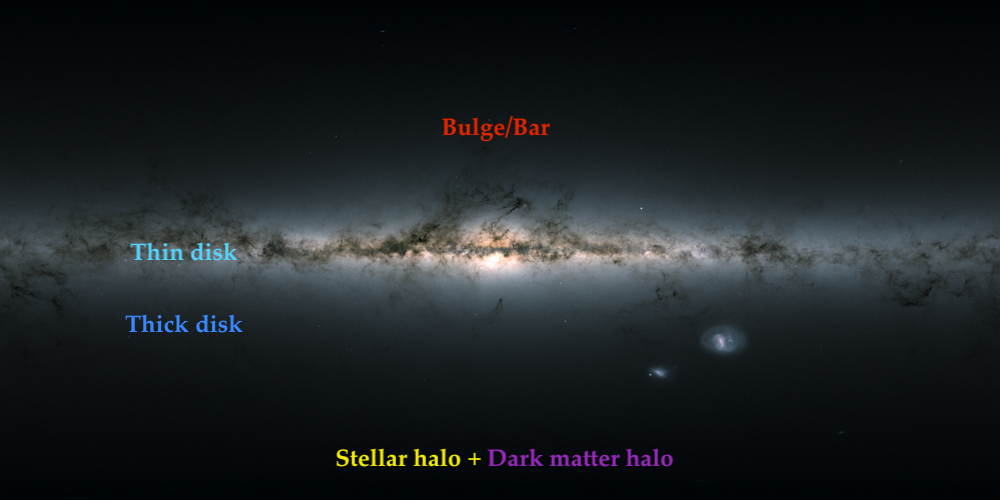
\includegraphics[width=1\textwidth]{images/gaiasky.png}
    \caption{All-sky view of the Milky Way Galaxy from Gaia based on measurements of nearly 1.7 billion stars. We mark the location of different components of the Galaxy with different colors. Image adapted from \textit{Gaia} Data processing and Analasys Consortium (DPAC) (CC BY-SA 3.0 IGO).} % Fig. 1.1
    \label{fig:gaiasky}
\end{figure}
All throughout history mankind has sought to understand the night sky and its many features such as stars, clumps, planets or `wanderers'. But no feature is as large and noticeable as the great spray of stars that make up the Milky Way Galaxy, named so for the milk from Hera's breast in Greek mythology \citep{leeming:98}. The suggestion that this milky band of stars was a rotating body, of which we the observers are inside, came not until \cite{wright:1750}. Since then our understanding of our home Galaxy has increased tremendously and we can present stunningly detailed views of it like the map shown in Fig. \ref{fig:gaiasky}. This map is made possible thanks to measurements from Gaia's second data release (\citealt{dr2},  herafter DR2). As the figure shows the Milky Way is composed of several different components with stars differing in spatial distribution, kinematics, chemistry, and age. Since the three papers together touch upon almost every component mentioned in Fig. \ref{fig:gaiasky} we will briefly provide a description of each one.

\subsection{Thin disk}\label{subsec:components-thindisk}
The thin disk is what visually makes up the Milky Way and since it is where the Sun is located it is the the most well-studied of the stellar components. The thin disk is also the site of ongoing star formation which recent estimates place as high as $\approx 3.3\ \mathrm{M_\odot yr}^{-1}$ \citep{zari:22}. As the name suggests it is relatively thin with a scale length of $R_\mathrm{t} \approx 2.6$ kpc, scale height of $z_\mathrm{t} \approx 300$ pc, and with a mass $M_\mathrm{t} \approx 3.5\times 10^10$ M$_\odot$ \citep{bland-hawthorn:16}. The thin disk stars are generally younger and has an abundance of $\alpha$-elements similar to the sun. We measure the abundances as:
\begin{equation}
    [\alpha/\mathrm{Fe}] = \log_{10}\left(\frac{N_\alpha}{N_\mathrm{Fe}}\right)_\mathrm{star} - \log_{10}\left(\frac{N_\alpha}{N_\mathrm{Fe}}\right)_\odot,
\end{equation}
where $N$ is the number of atoms per unit of volume.

\subsection{Thick disk}\label{subsec:components-thickdisk}
The second disk of the Galaxy fulfills its name with a scale height of $z_\mathrm{T}\approx 900$ pc, scale length $R_\mathrm{T} \approx 2$ kpc, and mass $M_\mathrm{T} \approx 6$ M$_\odot$ \citep{bland-hawthorn:16}. It's stars are older \citep{martig:16} and kinematically hotter, since age and velocity dispersion are correlated (\citealt{martig:14,aumer:16}). In metallicity space, thick disc stars occupy regions of higher [$\alpha$/Fe] and have been tentatively linked to the high-$\alpha$ sequence \citep{katz:21}. How the thick and thin discs formed is still a debated topic, particularly so the former as explained in \cite{helmi:20} who also shows that the formation may be related to the evolution of the stellar halo through mergers with nearby galaxies. 

\subsection{Stellar halo}\label{subsec:components-stellarhalo}
The most extended component is the stellar halo which contains $1.3^{+0.3}_{-0.2} \times 10^9$ M$_\odot$ within $2 < r < 70$ kpc \citep{mackereth:20} and is host to the oldest and most metal-poor stars in the Galaxy \citep{dacosta:19, horta:22}. The orbits of halo stars is more spherical than the disks and so can be told apart locally by their kinematics. Relative to the discs, the halo stars will appear to move with a speed of 200 km s$^{-1}$. The most commonly held formation pathway for the Milky Way is through hierarchical growth through several minor and major mergers, a model called $\Lambda$CDM \citep{springel:05}. This view matches well with current understanding of the stellar halo as having an \textit{in situ} component of stars as well as an accreted component which becomes extremely dominant at larger distances from the disk \citep{naidu:20}. It has also been shown that this accreted component has a plethora of substructures in it attributed to various accreted stellar populations (e. g. \citealt{koppelman:19, feuillet:21, dodd:22}). We will touch more upon this in sections \ref{sec:p3-gaiaview} and \ref{sec:p3-structures}.

\subsection{Dark matter halo}\label{subsec:components-darkhalo}
There is another halo which is not visible to our telescopes. If we only look to the stellar matter of a galaxy like the Milky Way, the rotational velocity of stars is expected to decrease with distance in a similar fashion to Keplerian rotation, in which $v_\mathrm{rot}^2 \propto M/R$. This is not what we observe however, and instead the rotation curve flattens out which is attributed to the existence of a dark matter halo. Current results place the mass of the dark matter halo at $M_\mathrm{dh} \approx 1.3 \times 10^12$ M$_\odot$ \cite{posti:19} and its shape is still a topic of much debate as explained in \cite{mcmillan:17}. While the debate goes on, it is very common in simulations to assume a spherically symmetric halo (e. g. \citealt{andersson:20}).

\subsection{The bulge}\label{subsec:components-bulge}
In the central regions of the Galaxy lies the bulge, heavily obscured by dust as is clearly visible in Fig. \ref{fig:gaiasky}. The nature of the bulge \textit{as a bulge} is uncertain. The idea of a spherical, so-called \textit{classical bulge} built up through early mergers makes sense given the old ages of bulge stars \citep{clarkson:08}. Following star counts in the bulge, it has been established that the bulk of the bar participates in a \textit{box/peanut}-shaped structure, related to the three-dimensional Galactic \textbf with cylindrical rotation (\citealt{wegg:13, ness:13b}). It us unclear if the Milky Way even has a classical bar. \cite{shen:10} uses the kinematics to constrain its contribution to be less than 8\% of the disk mass and it has been shown that the bulge has several different metallicity populations \citep{ness:13a}. There is evidence to suggest that parts of the bulge is formed from the Galactic disk \citep{dimatteo:19} through interactions that slowly rearrange energy, angular momentum, and mass, otherwise known as \textit{secular evolution} \citep{kormendy:13}.

\section{The bar \& spiral arms}\label{sec:barspirals}
\begin{figure}[t]
    \centering
    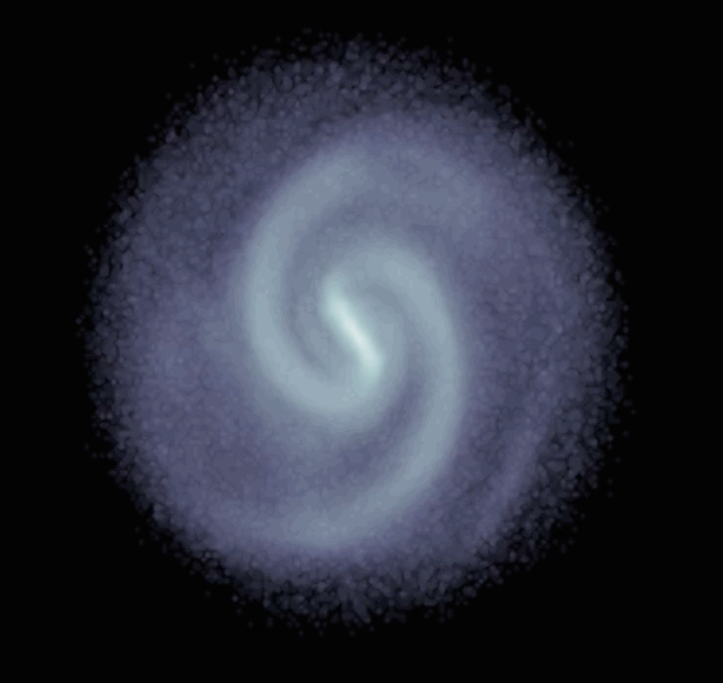
\includegraphics[width=.65\textwidth]{images/simgal.png}
    \caption{An example of a simulated Milky-Way like disc Galaxy with pronounced spiral arms and a central bar.} % Fig. 1.2
    \label{fig:simgal}
\end{figure}
Beyond the components mentioned in the previous sections, there are the non-axisymmetric features. In other galaxies they are clearly visible but since we reside inside our Galaxy we struggle to see them as clearly. As an example we show a simulated galaxy in Fig. \ref{fig:simgal} which has a bar and two spiral arms that can be seen very clearly and represents a typical disc galaxy. Since non-axisymmetric features play an important role in secular evolution we will take a closer look at these features in the Milky Way.

The boxy/peanut shaped bulge mention in section \ref{subsec:components-bulge} is an inner, vertical extension of the Galactic bar \citep{bland-hawthorn:16}. The bulge region reaches to about ${\sim}2$ kpc \citep{wegg:13} while the bar may reach as far as 5 kpc \citep{wegg:15}. For this reason it is sometimes referred to as the `long' bar. Current estimates for the bar puts it at ${\sim}1.6\pm 0.3 \times 10^10$ M$_\odot$ \citep{kipper:20} and using Gaia's third data release (\citealt{dr3}, hereafter DR3) the bar angle with respect to the Sun-Galactic Centre (GC) is estimated to be $-19.2^\circ \pm 1.5^\circ$ \citep{dr3:asymmetries}. The bar is not static however and is rotating with a specific angular velocity, called pattern speed. The pattern speed of the bar is subject to much debate with many attempts at determining it. In \cite{bland-hawthorn:16} they review many of the estimates and conclude with an estimated pattern speed of $\Omega_\mathrm{b} \simeq 43 \pm 9$ km s$^{-1}$ kpc$^{-1}$. More recent estimates place the pattern speed of the bar at $\Omega_\mathrm{b} = 33.29 \pm 1.81$ km s$^{-1}$ kpc$^{-1}$ \citep{clarke:22}, in agreement with the previous value. These scales of pattern speeds has been called a `slow' bar scenario.

The other major non-axisymmetric feature of the Milky Way are the spiral arms. They likely travel around the whole disk and as such, we do not have a full picture of them to date and instead must look to whatever parts of them are visible to us from our position as observers in their plane. Current belief within the community is that the Milky Way has four approximately symmetric spiral arms \citep{vallee:17} rather than just two. The names for these four arms as in literature are \textit{Perseus}, \textit{Sagittarius-Carina}, \textit{Scutum-Centaurus}, and \textit{Norma-Outer}. The sun is believed to lie inside of \textit{Perseus}, and just outside \textit{Sagittarius-Carina} in an inter-arm region. In addition to these arms, very close to the Sun lies the \textit{local arm}, initially believed to be a spur of the \textit{Perseus arm}. It has since been understood to be fifth feature with comparable qualities to the other major arms. In spiral galaxies the highest densities of gas and stars lie along the arms which is the site for most star-formation in the disk. 

\section{Radial migration}\label{sec:migration}
\begin{figure}[t]
    \centering
    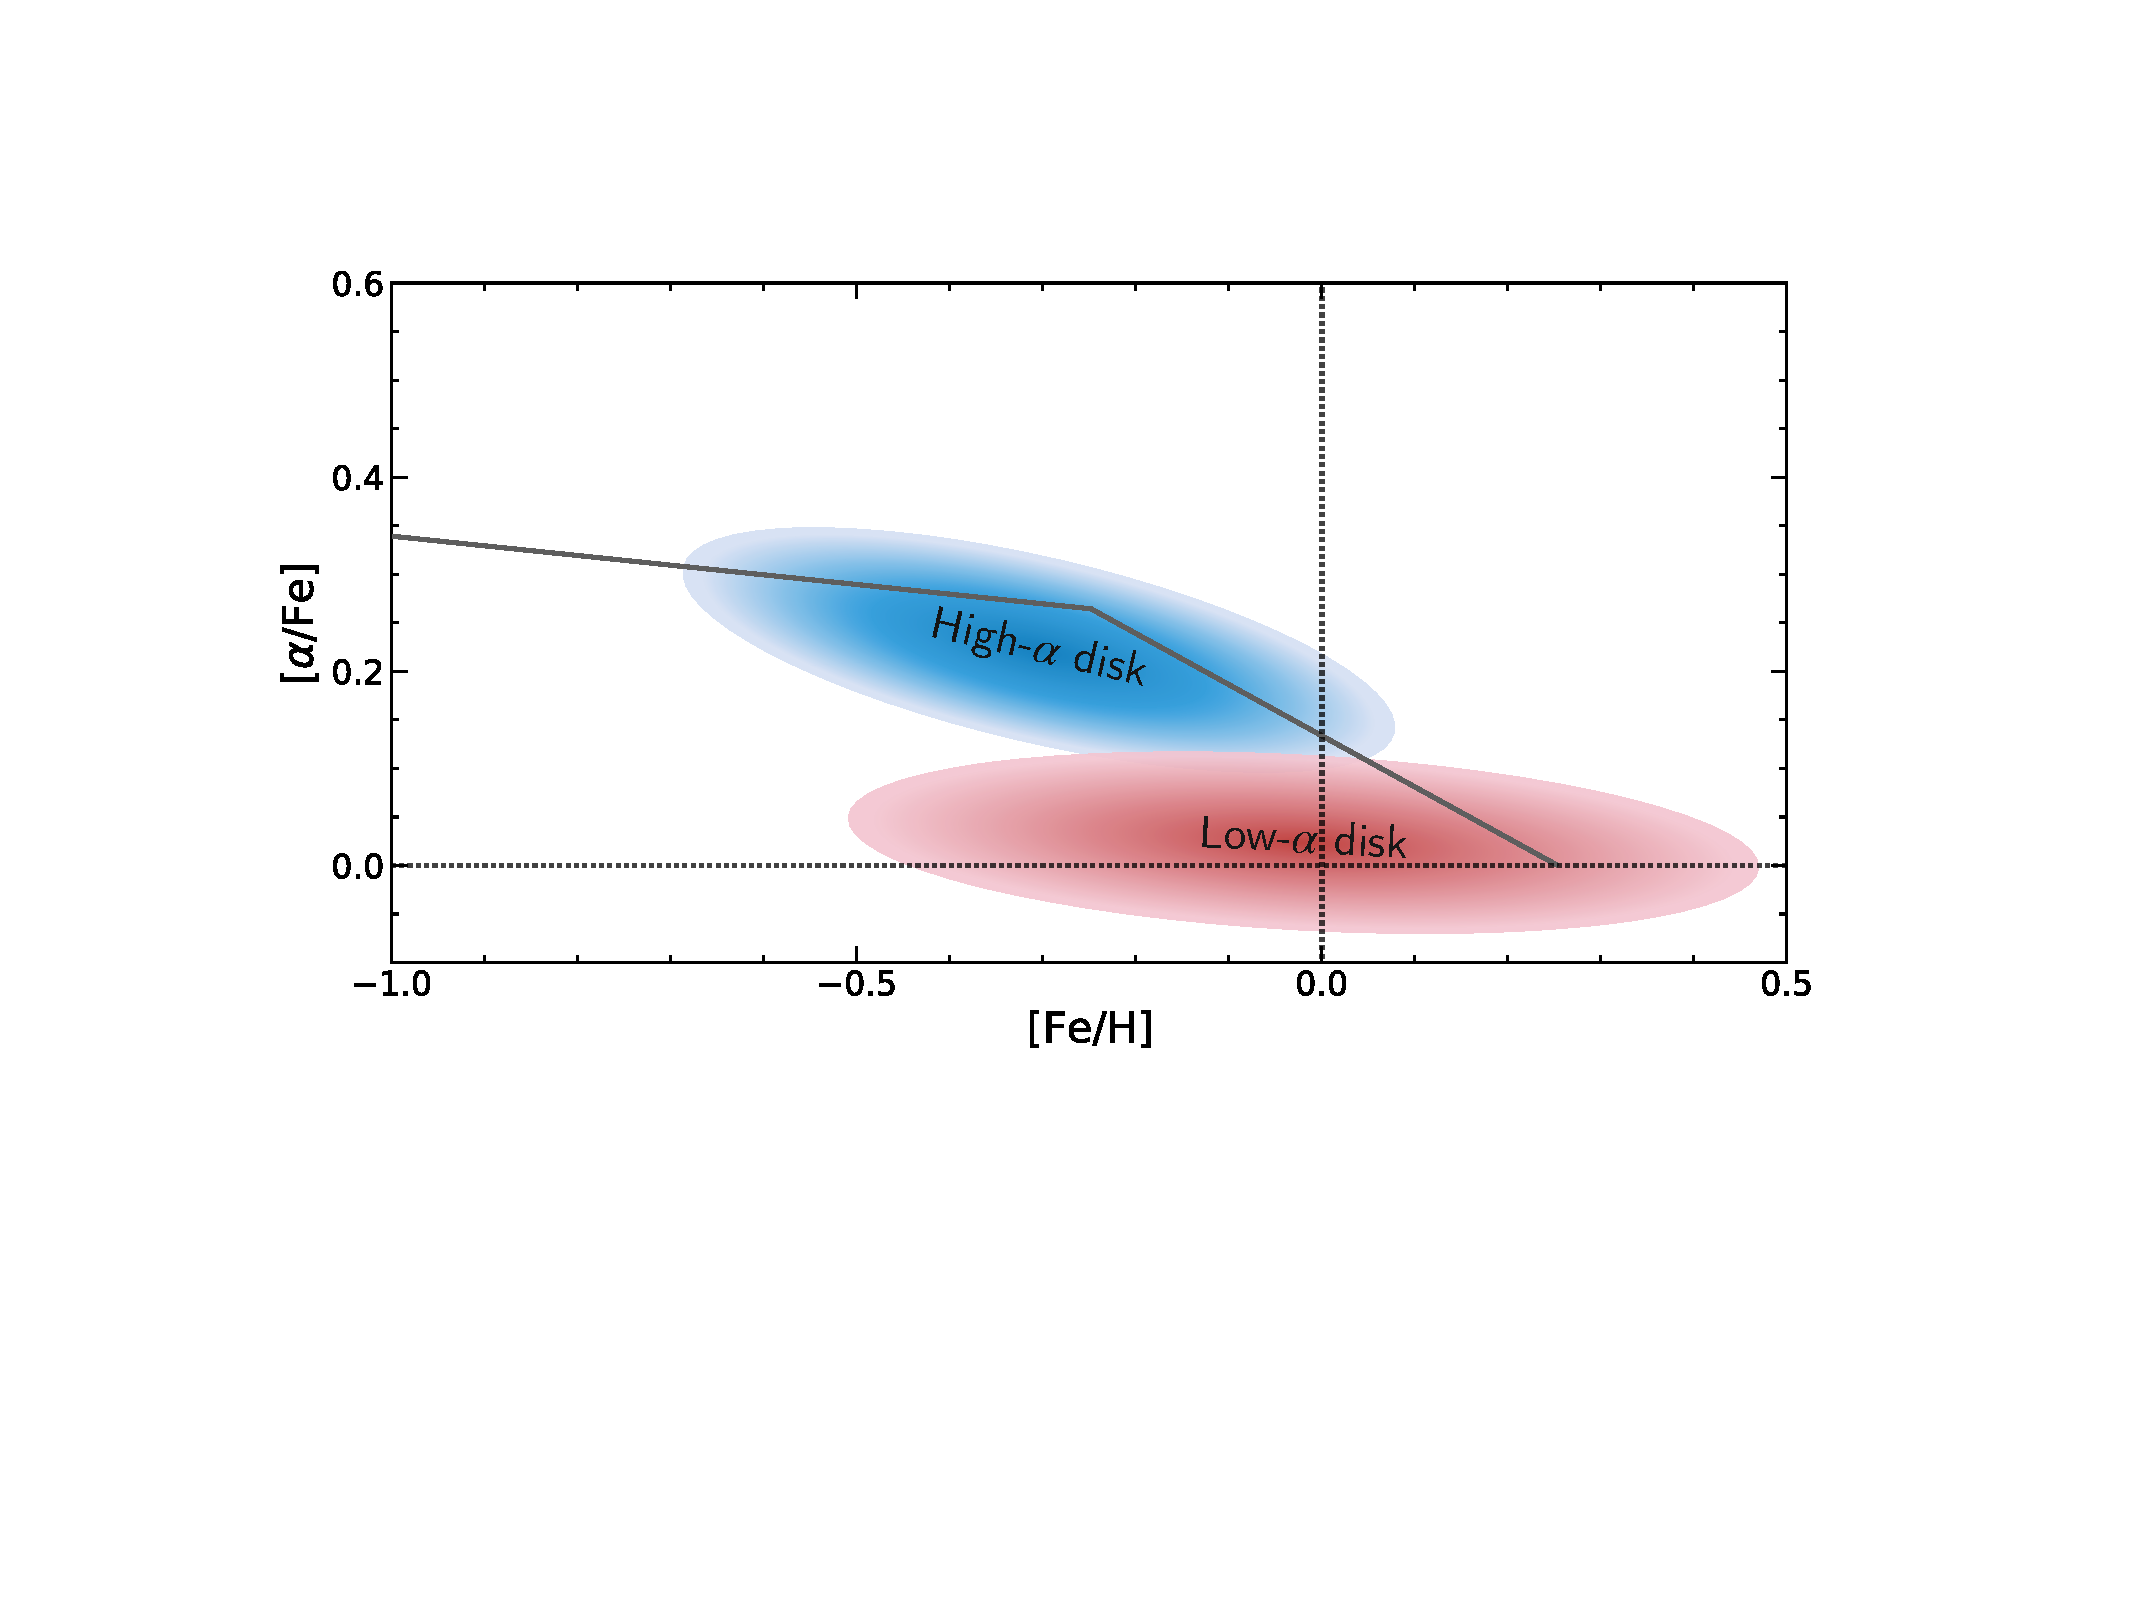
\includegraphics[width=.9\textwidth]{images/alphaoverfe.pdf}
    \caption{An illustration of the distribution of abundance of $\alpha$-elements vs the abundance of iron. The dotted line shows the location of the Sun and the gray solid line the expected evolution of an isolated region of the ISM.} % Fig. 1.3
    \label{fig:alphaoverfe}
\end{figure}
Since the spiral arms and the Galactic bar are such very prominent features of our Galaxy and in other similar spiral galaxies, it is no surprise that they have a profound impact upon the disc in which they are found and the stars that live therein. One such effect which occurs because of the dynamical interplay between disk and the non-axisymmetric features is \textit{radial migration}, which is the displacement of a star in the radial direction of its galactic plane. We will soon explain the mechanics of the major processes which cause radial migration but first the importance of radial migration as an ingredient of galaxy evolution, and the evidence to support it, should be discussed.

Let us consider the chemical evolution of the Galactic disc. The abundance of $\alpha$-elements and Fe over time in an isolated region of the interstellar matter (ISM) are affected by the life and death of its stars through what is called stellar nucleosynthesis (for a review see \citealt{edvardsson:1993}). In short, stars create elements and enhances the abundances of the next generation. Initially core-collapse supernovae produce similar amount of $\alpha$ and Fe, but [Fe/H] increases. Eventually type Ia supernovae begin, which produces Fe but no $\alpha$-elements and thus for the region [$\alpha$/Fe] starts to drop. This behaviour produces a trend like the gray line seen in Fig. \ref{fig:alphaoverfe}. If we are in a very isolated region, we would expect to see that the stars follow this narrow trend. Neighbouring regions radially inside and outside of the region would however have higher and lower [Fe/H] ranges as it has been shown that [Fe/H] increases radially inwards in the Galaxy \citep{hayden:15}. In observations of the Solar neighbourhood (e. g., \citealt{edvardsson:1993, hayden:15, bensby:14},) we see a range of different Fe abundances at each [$\alpha$/Fe], similar to the illustration shown in Fig. \ref{fig:alphaoverfe}. Similarly, the age-metallicity relationship (AMR) can be expected to follow a narrow line for this region, but shows a wide scatter. This can be quite easily explained if the different regions of the disc are not isolated from each other, but rather there is radial mixing between them. Beyond this rather straight-forward example of radial migration, several other observed features of the Milky Way disc has been suggested to be caused by it as well such as the observed bimodality in plots like Fig. \ref{fig:alphaoverfe} \citep{schonrich:09, toyouchi:2016} and the flaring of the outer disk in mono-age populations \citep{minchev:12}. It is clear that some form of radial migration is occurs in the Milky Way and we are today even able to estimate the radial displacement of individual stars as in \cite{frankel:18} which finds that the Sun as well has likely migrated from a birth radius of {$\sim$}5.2 kpc. Therefore it is important to understand the processes by which migration occurs.

\subsection{Radial heating}
\begin{figure}[t]
    \centering
    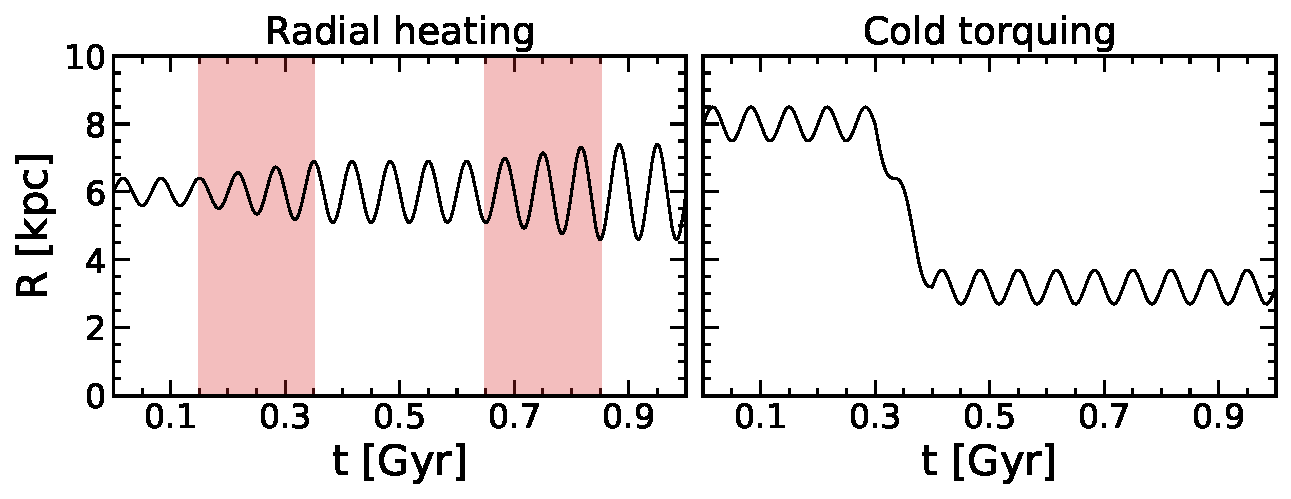
\includegraphics[width=1\textwidth]{images/radialmigration.pdf}
    \caption{A simple sketch of the radius evolution of an orbit that undergoes radial migration. \textit{Left}: Shows the effect of radial heating or blurring, which increases or decreases the amplitude of the radial oscillations of the orbit. The shaded regions mark the time during which the radial heating occurs. The guiding center radius, $R_g$, is never changed during the process. \textit{Right}: The effect of cold torquing or churning on an orbit, which displaces the guiding center radius, $R_g$, but does not increases the amplitude of oscillations and therefore does not increase the radial action, $J_R$.} % Fig. 1.4
    \label{fig:radialmigration}
\end{figure}

One rather simple cause of radial migration is what is called \textit{radial heating}, sometimes called \textit{blurring}. Stars are born in Giant Molecular Clouds (GMCs) which move on nearly circular orbits around the disk. This means that the stars themselves are born on nearly circular orbits. But through the evolution of stellar orbits they can scatter by interaction with things like other GMCs or clusters which will lead them onto eccentric orbits, called \textit{epicycle orbits} as they are described by the \textit{epicycle approximation}. The epicycle refers to the radial oscillations of the perturbed orbit, occuring with an \textit{epicycle frequency}, $\kappa$. The reason a perturbed star does not simply move to a different radius when scattered is because of the fine balance between centrifugal and gravitational force keeping it in place. If the star is pushed radially outwards, the centrifugal force decreases faster than gravity and the star moves back in. The star now overshoots to an interior radius where the centrifugal force increase faster than gravity which pushes it back out. In other words we say that the star is stable to small velocity changes. Because of the oscillations the star will visit different radii than its original radius, called the \textit{guiding radius}, $R_g = L_z / v_c$, where $L_z$ is the angular momentum perpendicular to the disk and $v_c$ is the circular velocity. It is the process of increasing the amplitude of the oscillations that we call radial heating and we show how this might look in the left panel of \ref{fig:radialmigration}. 

Given that the stars visit other regions of the Galaxy, they can obviously enrich those regions as well which leads to the conclusion that radial heating can contribute to the width observed in the chemical evolutionary tracks discussed in the previous section. It can be shown as in \cite{binney:07} however that radial heating will only account for around 50\% of the observed scatter in the metallicity and instead there must be some additional source of mixing to explain the measured scatter. 

\subsection{Cold torquing}
\begin{figure}[t]
    \centering
    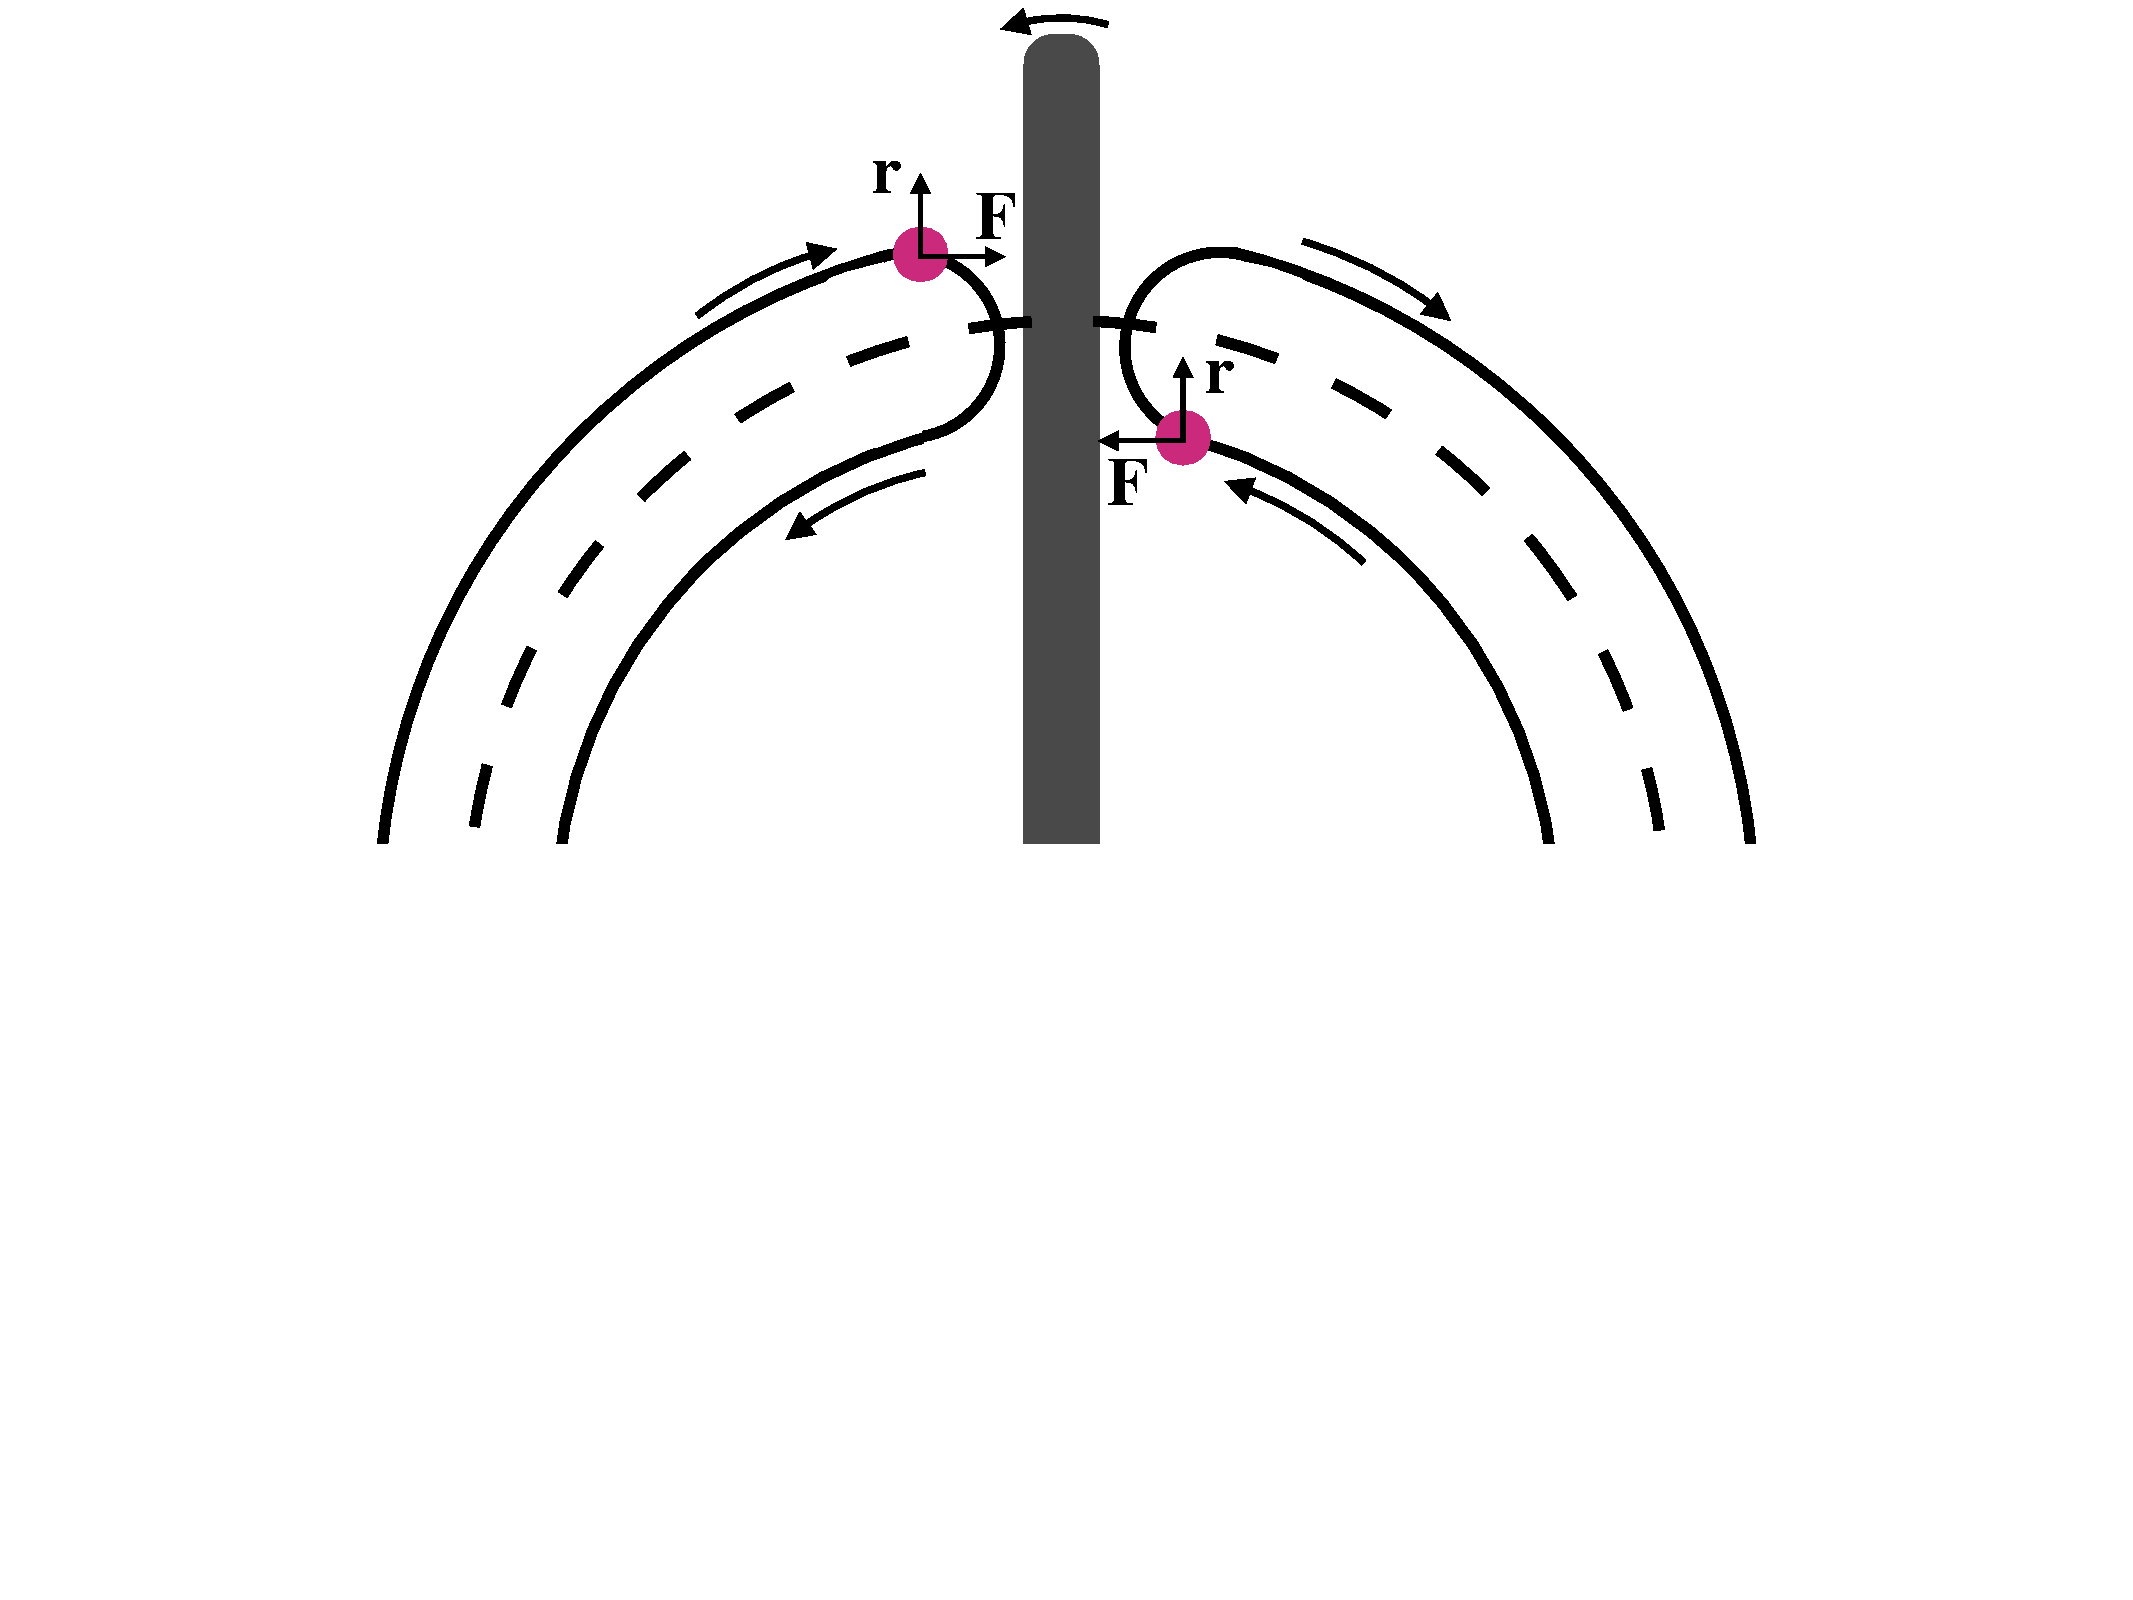
\includegraphics[width=0.8\textwidth]{images/torquing.pdf}
    \caption{The concept of horseshoe orbits and angular momentum transfer near corotation of a non-axisymmetric feature with constant angular speed. The dashed line marks the corotation radius and the pink points are positions along the horseshoe orbit right before angular momentum transfer. The vectors for $\pmb{r}$ and $\pmb{F}$ which gives the torque is indicated} % Fig. 1.5
    \label{fig:torquing}
\end{figure}
Another source of radial mixing was described first in a seminal paper by \cite{sellwood:02} wherein it was shown that disk heating is not the dominant effect of the spiral arms. Instead, non-axisymmetric features like the bar and spiral arms are able to shift the guiding radii of stars without significantly altering their dynamics. This processes occurs through resonant interactions with the non-axisymmetric features. The spiral arms or bar will exert a torque that changes the angular momentum of the star's orbit since:
\begin{equation}
    \frac{d}{dt}\pmb{L} = \frac{d}{dt}(\pmb{r}\times\pmb{p}) = \pmb{r}\times\pmb{F} = \pmb{\Gamma}.
\end{equation}
Axisymmetric features like bars and spirals move with constant angular velocity, which means that the non-angular velocity increases further out. This means that for stars with approximately constant circular velocity there is a radius at which the velocity of a star and spiral/bar is the same, called \textit{corotation}. Beyond this point stars move more slowly than the spiral and within it they move faster. Faster stars catch up to the feature and will have a force, $\pmb{F}$, directed towards it. Slower stars instead fall into it with a force in the opposite direction. We illustrate this in Fig. \ref{fig:torquing} which shows that for the fast stars, the torque will be directed inwards, i.e., negative which decreases the angular momentum and transfers it to a smaller $R_g$ orbit where it moves faster. It eventually catches up to the spiral/bar and is given a positive torque, migrating outwards. 
\chapter{Paper I}\label{chap:paper1}
\section{Introduction}\label{sec:p1-intro}

\section{Setting up simulations}\label{sec:p1-simulations}

\section{Evolution of non-axisymmetric features}\label{sec:p1-evolution}

\section{Quantifying radial migration}\label{sec:p1-quantifying}
\chapter{Motions of stars}\label{chap:motions}
\begin{flushright}
\textit{``The stars are far brighter, Than gems without measure."}

- J. R. R. Tolkien, The Hobbit
\end{flushright}
\section{The oldest science}\label{sec:oldest}
\begin{figure}[t]
    \centering
    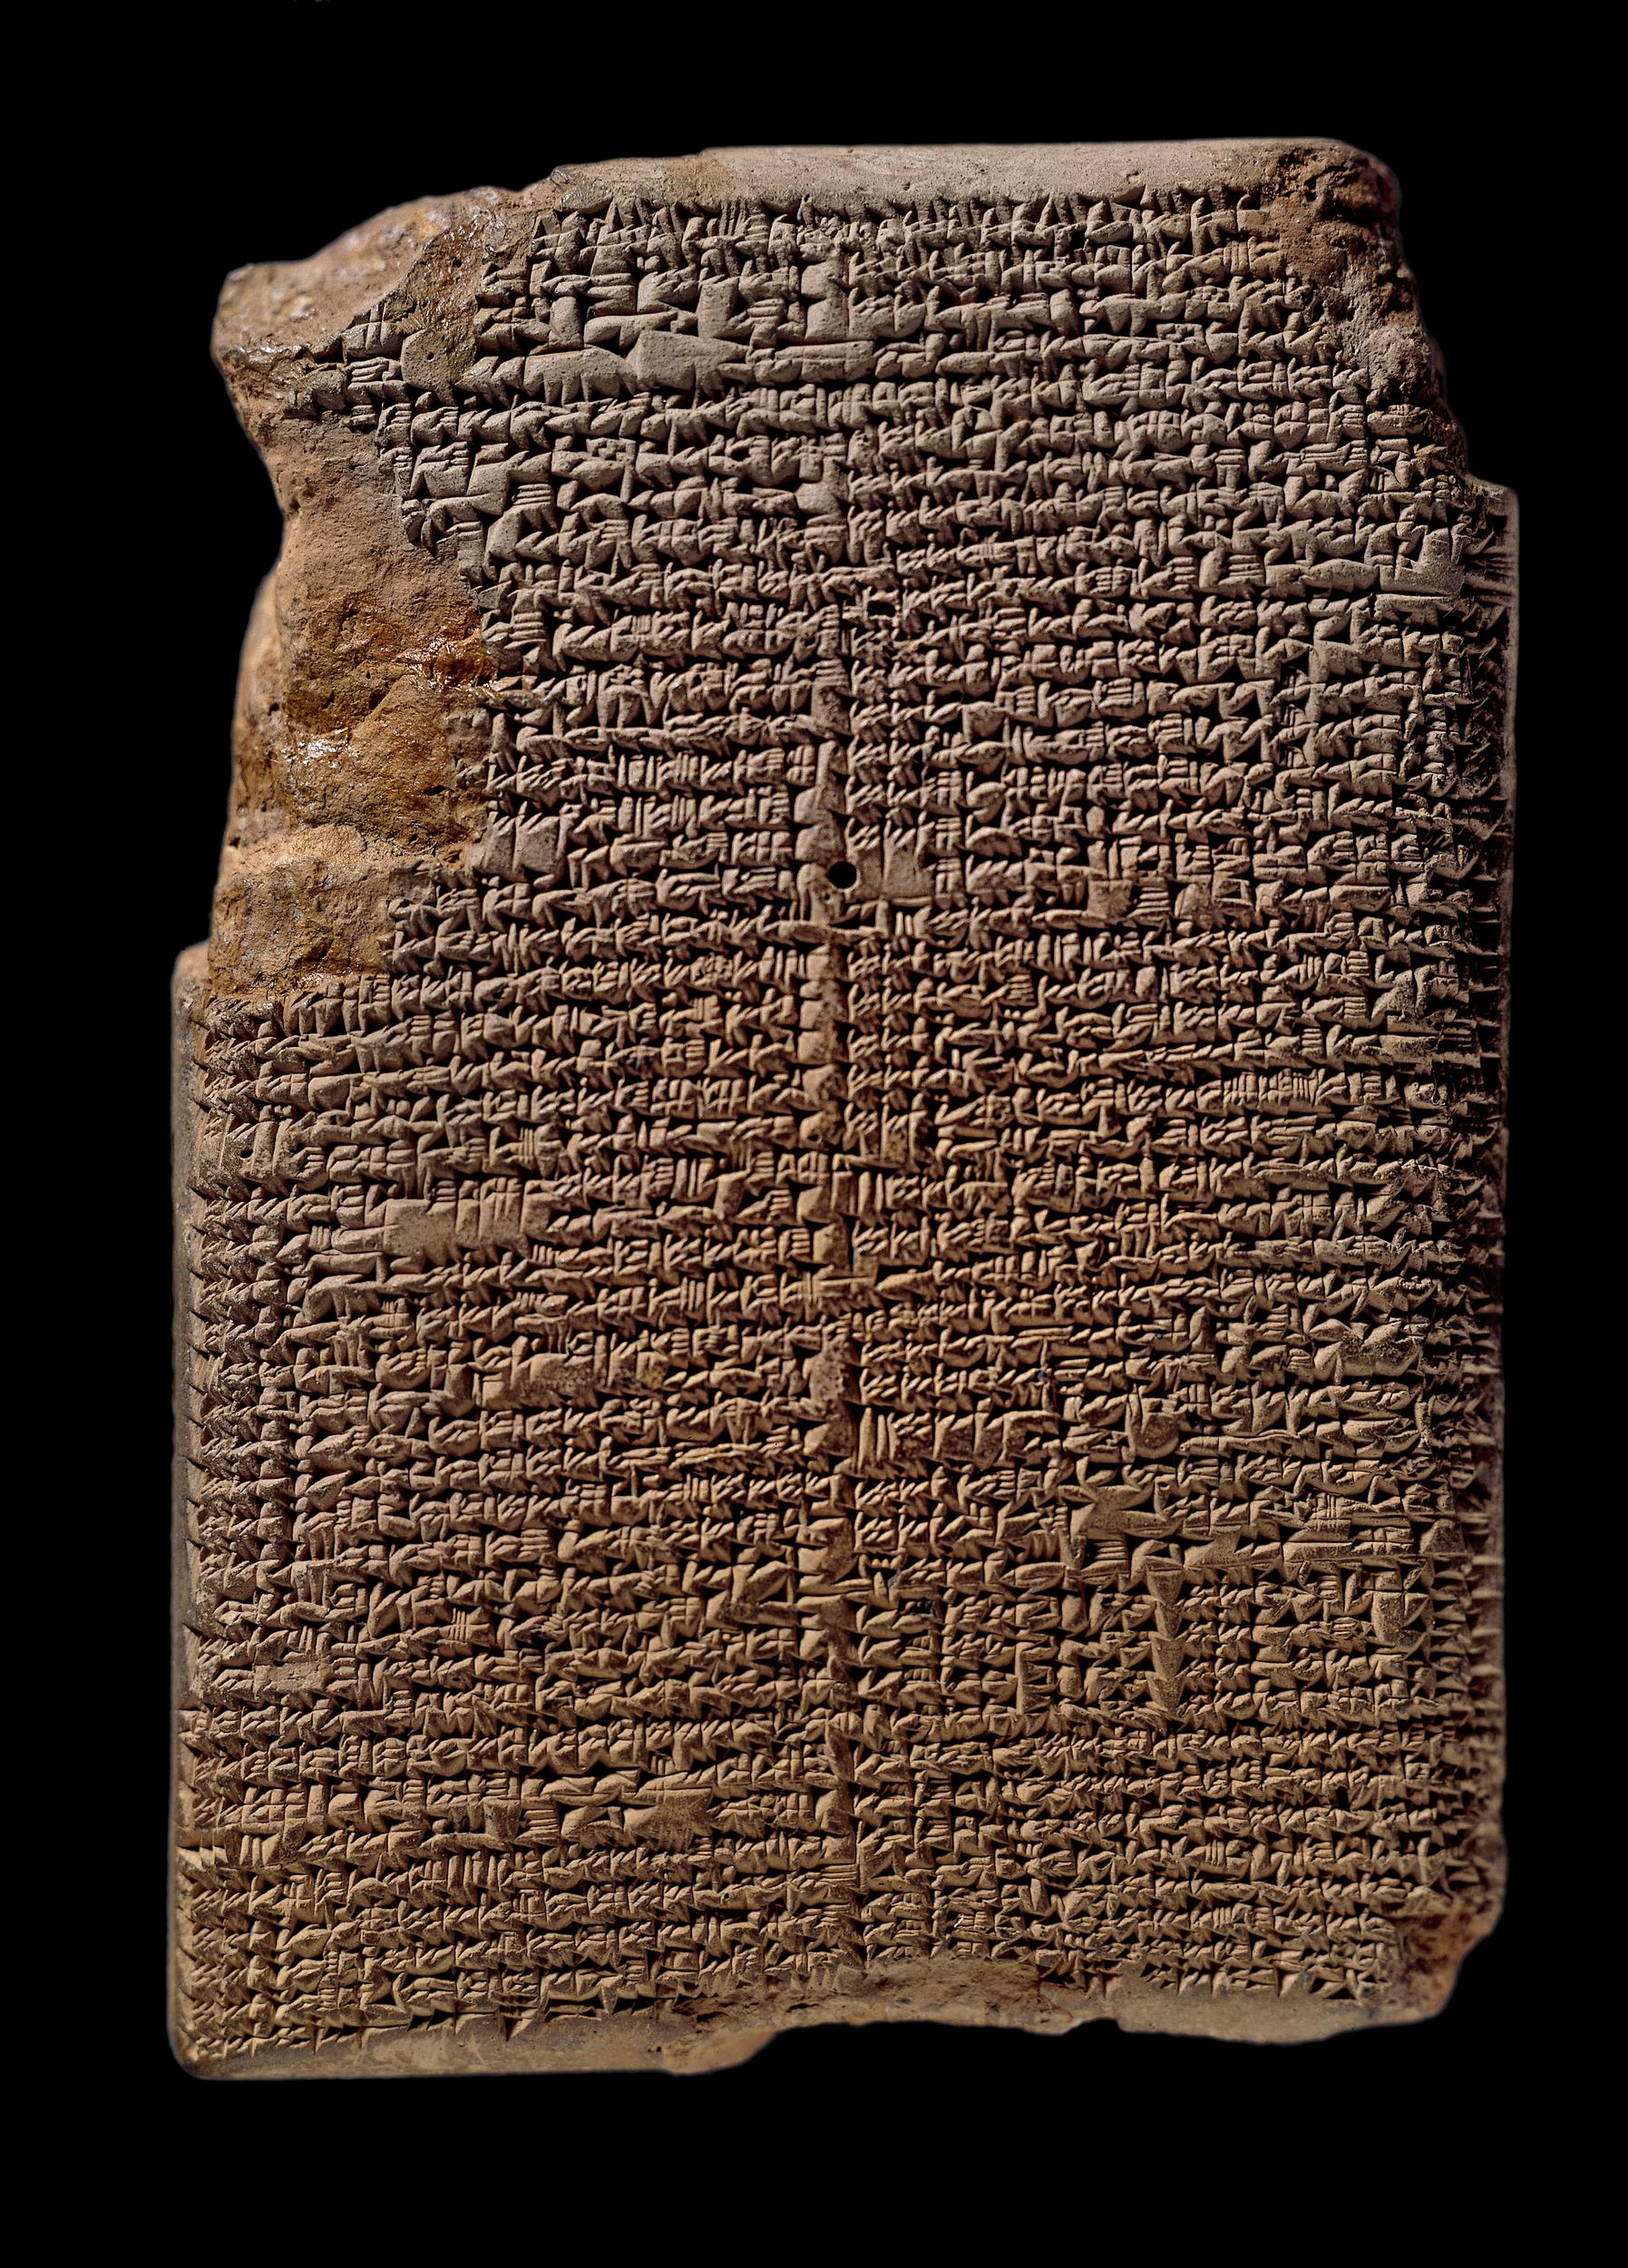
\includegraphics[width=0.4\textwidth]{images/tablet.jpeg}
    \caption{The Mul-Apin clay tablet, tablet 1. The tablet has sections locating constellations in relation to each other and lists stars and constellations according to celestial latitude among other entries. © The Trustees of the British Museum. Shared under a Creative Commons Attribution-NonCommercial-ShareAlike 4.0 International (CC BY-NC-SA 4.0) licence.} % Fig. 3.1
    \label{fig:tablet}
\end{figure}
The fascination of mankind with the celestial sphere has undoubtedly been around for far longer than historical records can demonstrate. Beyond a scientific curiousity, the night sky has had practical purposes that have been used throughout history. Polaris points the way north for travellers of all sorts. The blurring of stars can tell sailors that it is windy at sea. Agriculture heavily relies on the use of calendars based around the Sun and Moon. The relationship between astronomy and humans was arguably more tangible and transparent in the past than it is today, when non-astronomers do not need to think about these matters very often. 

In the last few decades, the study of prehistoric astronomy has boomed into its own field called archaeoastronomy, and revolves around the study of prehistoric sites and their possible astronomical association (see \citealt{magli:20} for a review). These sites have origins dating back several millenia BCE. The earliest historically verified accounts of astronomy comes from Mesopotamia and the ancient kingdoms of Sumer, Assyria, and Babylonia. From this region has been found clay tablets noting down positions and locations for constellations and planets. One significant example of such is the \textit{Mul-Apin} clay tablet, shown in Fig. \ref{fig:tablet}, which dates back to a little over 1000 BCE \citep{dejong:07}. 

Around 200 BCE the first star catalogue was made by \textit{Hipparchus} in ancient Greece\footnote{The history of astrometry is described in much greater detail in \cite{perryman:12} than it is here and we encouraged the interested reader to have a look.}. This catalogue contained positions of stars and is often linked to the birth of \textit{astrometry} as a subject, the study of positions and movements of celestial bodies with precise measurements. As the Roman empire fell and the Dark Ages began, astrometric advances were made to wait. In 1428 a 36-meter sextant was constructed in Uzbekistan by the grandson of the Mongol conqueror Tamarkand, \textit{Ulugh Beg}. This provided a new star catalogue of 994 stellar positions accurate to a degree. The next advancement came from Scandinavia as \textit{Tycho Brahe} (1546-1601) on the Danish island of Hven, using a quadrant of around seven meters at his Uraniborg observatory, measured a thousand stellar positions. His accuracy reached about 20\as. In order to perfect the art of navigation, it was necessary to determine longitude of various places. For this purpose the Royal Greenwich Observatory was founded in 1675 and its first Astronomer Royal was \textit{John Flamsteed} (1646-1719), tasked with determining the motions of the heavens. After his passing was published a catalogue of 2935 stellar positions accurate to 10\as-20\as, the \textit{Historia Coelestis Brittanica} \citep{flamsteed:1725}, the first catalogue using a telescope. This expanded rapidly thereafter and had reached 50 000 stars with 3\as accuracy in \textit{Histoire Céleste Française} by \textit{Jérôme Lalande} (1732 - 1807) \citep{lalande:1801}. 

The next step is not an increasingly large catalogue. Instead, through separate works by \textit{Wilhelm Struve} (1793-1864), \textit{Friedrich Bessel} (1784-1846), and \textit{Thomas Henderson} (1798-1844) the first stellar parallaxes were published between 1837 to 1839. The parallax is the apparent angular displacement of an object due to the displacement of the observer. When driving down a highway, you will notice that as you move, the mountains in the background move more slowly across your field of vision than the trees by the side of the road. This angular displacement is the parallax, larger for nearby objects, smaller for more distant ones. The same can be done for the stars, as the closer a star is the more it is displaced across the celestial sphere as the Earth orbits the Sun. The distance to stars based on their apparent motions could now be measured, albeit for individual stars at first. It is worth nothing the scale of these distances. Bessel's measurement of 61 Cygni's parallax was 0.314\as, corresponding to ${\sim}3$ pc or roughly 90 trillion kilometers. The enormity of the Universe could no longer be questioned. During the next century and a half, the number of available ground-based parallax measurements grows rapidly and culminates in 1995, when the \textit{Yale Trigonometric parallax Catalogue} is published by \textit{William van Altena} \citep{vanaltena:95}. The parallax measurements are then limited to an accuracy of 0.5\as\ due to the flickering of the Earth's atmosphere which is reduced to 0.01\as\ when averaging over many measurements. One workaround is adaptive optics, distorting the mirror to compensate for the atmosphere, which is used in the \textsc{gravity} instrument \citep{gravity:11} to achieve up to 0.003\as. Even then however, the entire sky cannot be covered. Furthermore, it is not the most precise astrometry we can get. Further precision requires that the next advancements be made using space telescopes.

\section{Hipparcos \& Gaia}\label{sec:gaia}
In 1989, following a little over two millennia of astrometric catalogues, the first astrometric satellite was launched by ESA with the name \textit{Hipparcos}, named after the author of the first catalogue. Eight years later the catalogue was published in \cite{perryman:97}, containing positions, proper motions (the on-sky angular motions), and distances for 117 955 stars, accurate to a milliarcsecond (mas). This mission was also used to produce the lower-precision Tycho catalogue (named for Tycho Brahe), which expanded the number of stars with proper motions and positions to 2.5 million \citep{hog:00}. The scientific gifts of Hipparcos were many, and the achievements made possible are reviewed in \cite{perryman:09}. 

The opportunities awarded to astronomers by Hipparcos perhaps left the community hungry for more because not long after, in 2013, its successor was launched and was designed to provide the single largest improvement on past available astrometry, by a wide margin. This mission is called \textit{Gaia} \citep{gaia} and currently provides the largest available set of astrometric data. 

The Gaia mission has so far had three full data releases (DRs). DR1 \citep{dr1} released with the five-parameter astrometric solution (positions, parallax, proper motions) for 2 million sources. The total number of sources was closer to 1.1 billion, but getting the astrometric solution using one year's worth of data required the adoption of the \textit{Tycho-Gaia Astrometric Solution}, described in \cite{michalik:15}. Two years later DR2 \citep{dr2} released with {$\sim$}1.3 billion five-parameter sources. Not only that, but the onboard spectrometer provided {$\sim$}7.2 million radial velocities, completing the full 6D phase-space information for these stars in addition to 3D position with on-sky velocities. Two years later again, the Early Data Release 3 \citep{edr3} arrived with five-parameter solutions for {$\sim$}1.4 billion sources. The radial velocities came with DR3 \citep{dr3} and we now have {$\sim$}33 million sources with RVs. The precision of Gaia is of course also a massive improvement on that of previous catalogues. From brightest to faintest sources, Gaia now has an uncertainty of 0.01-1 mas in position, and 0.02-1.3 mas in parallax, 0.02-1.4 mas yr$^{-1}$ in proper motion. The astrometry of the faintest stars is about as accurate as Hipparcos could provide for any star, and the ratio of sources in Hipparcos to those in Gaia is about $8\times 10^{-5}:1$, representing an increase of about 12 000 times. 

In addition to astrometry and spectroscopy, Gaia also provides photometry, variable sources, as well as some parameters for Solar system objects\footnote{For a more exhaustive list of everything in the data releases, see the `info' section of each release on \url{https://www.cosmos.esa.int/web/gaia/data}}. Gaia is not done quite yet and the future is sure to be exciting with a successor mission being planned which would conduct astrometry in the infrared \citep{hobbs:21}. It does not seem like the exponential growth of astrometry is stopping anytime soon, much to the benefit of our understanding of the universe.

For everything Gaia does well, we need to discuss a shortcoming of the data with respect to studying Galactic dynamics that is central to the work in Papers II and III. Radial velocities were not available in the Gaia catalogue until DR2, and when released was only available for about 0.5\% of the astrometric solutions. This was slightly improved with DR3, which reached closer to 2\%. This still leaves the vast majority of the data without 6D phase-space information. Full phase-space information is important because, as \cite{dehnen:98a} puts it, "\textit{The dynamical state of a stellar system is completely described by its phase-space distribution function $F(\bm{x}, \bm{v})$"}. Practically we cannot determine the full distribution in a realistic way, instead we seek to determine more local variations of the velocity distribution $f(\bm{v})$. 
\begin{figure}[t]
    \centering
    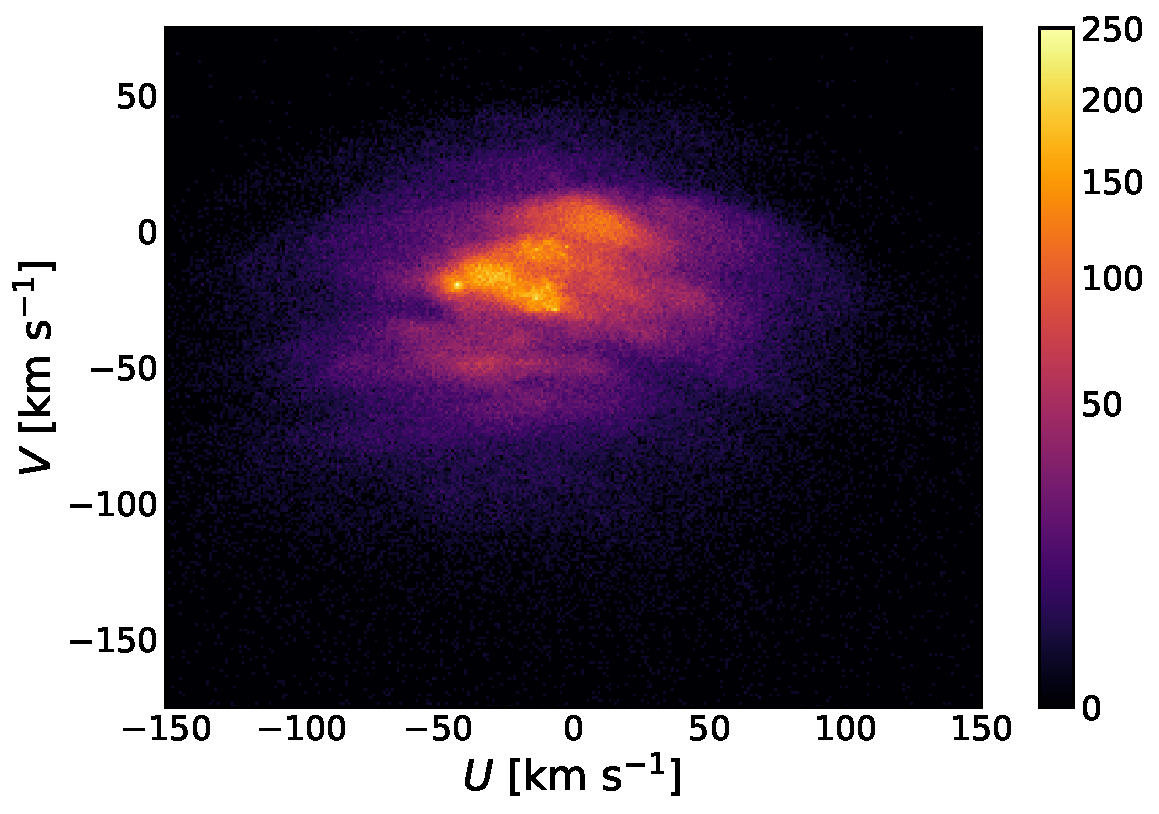
\includegraphics[width=0.8\textwidth]{images/dr3veldist.pdf}
    \caption{The number density distribution of sources from DR3 with radial velocities in the Solar neighbourhood. There is clearly a great deal of structure present already at close proximity to the Sun. The colorscale is shows $\sqrt{N}$ and the axes show Galactic velocities $U$, towards the Galactic centres, and $V$, in the direction of Galactic rotation.} % Fig. 3.2
    \label{fig:veldist}
\end{figure}

Now comes the issue; we do not have 3D velocities for the majority of these sources. How can we hope to determine the velocity distribution? To begin with, we can simply work with the sources that have radial velocities. This has been done of course and for DR2 it was in one of the demonstration papers, \citep{dr2:kinematics}. We use DR3 to recreate the same plot here, using a similar Solar neighbourhood sample we have around 500 000 stars, whereas in DR2 the sample contained {$\sim$}350 000 stars. The velocity distribution can be seen in Fig. \ref{fig:veldist}. This figure shows us that the velocity structure of the Galaxy, even locally, is anything but straight-forward. Structure in velocity space can be caused by a variety of processes \citep[see, e.g.,][]{antoja:10a}. Originally it was thought to come from disrupted stellar clusters. Newer suggestions have been accreted dwarf galaxies and close passings by external galaxies. Last but not least, the resonances of the spiral arms and bar, as discussed in the context of Paper I, can cause substructure in velocity space as well. We can with ease understand how decoding the velocity structure of the Galaxy will provide valuable insight into its evolution and history. It is therefore vital that we have access to as many stars as possible.

So what about the remainder of sources? It turns out that all hope is not lost. Already in \cite{dehnen:98a} the velocity distribution from Hipparcos was determined, despite the lack of radial velocities, by employing a clever approximation of a velocity distribution which is isotropic across the sky and then inferring $f(\bm{v})$ with a penalized maximum likelihood estimate (MPLE) (we will return to this in section \ref{sec:p2-inferring}). Similarly the average velocities and the velocity dispersion were determined in \cite{dehnen:98b}. Other studies that work around the absence of measured radial velocities include \cite{antoja:17} with estimates of disc velocity asymmetries, \cite{koppelman:21} who determined the Milky Way's escape velocity, and \cite{mcmillan:22} who looked to the outer parts of the disc near the anti-centre and showed that the velocities exhibit properties that match well with being perturbed by a dwarf galaxy. At least for now, it is absolutely necessary to use proper motion-limited samples if we wish to have access to catalogues that span a greater part of our Galaxy, and if we wish to have access to all kinds of stars. 

The astrometric renaissance is now and it is an exciting time for all fields of astronomy that can make use of the impressive data that is not only currently released, but is sure to arrive in the foreseeable future.

\chapter{Paper II}\label{chap:paper2}
\section{Introduction}\label{sec:p2-intro}
In Paper II we deal with the velocity distribution of local stars which was discussed in the previous chapter. Specifically, we determine the velocity distribution and velocity moments of Solar neighbourhood white dwarfs (WDs) in Gaia EDR3. In order to do this we make use of the methods derived in \cite{dehnen:98a} and \cite{dehnen:98b} which up until this point had not been employed for new data since Hipparcos. Since the method does not rely on any measurements of radial velocity the WDs are ideal candidates who very rarely have such measurements provided. 

The velocity distribution is a powerful tool to decode the evolution of the Milky Way's components as the community has been able to show in the past few decades. Recent research has been able to show a staggering amount of substructure in the velocity distributions \citep{antoja:12, kushniruk:17, dr2:kinematics} where we can see individual velocity structure up to hundreds of km s$^{-1}$ away from Solar motion as well as horizontal arches that span across the distribution. In addition to classical motions in $U, V, W$, the field has grown to include distributions in actions and angles, called orbit space (e.g., \citealt{trick:19, trick:21, trick:22}). In orbit space we can see clear ridges that are linked closely to the various structures in velocity space. Going forwards, both of these velocity spaces will be important to understand the dynamical structure of the Milky Way.

The WDs has, as mentioned, not been as easy to probe as the rest of the stars in the Solar neighbourhood. This leads to smaller samples which a couple of decades ago were only in the few hundreds \citep{sion:77, sion:88} and more recently samples which range from a couple of thousand to a few tens of thousands \citep{rowell:11, anguiano:17}. Recent works that investigate the kinematics of WDs are \cite{torres:19} who used Gaia to identify the \textit{Hercules} stream in the WDs and \cite{raddi:22} who determined the local kinematic properties of WDs. These samples are about as large as they come, with {$\gtrsim$}10 000 and {$\sim$}3000 for the two papers respectively. In my second paper, our method provides us with a sample of 129 675 WDs, the largest to date. We use this sample to identify known substructure as well as some novel features in velocity space. In addition to this, we also manage to identify two kinematically separate WD populations, attributed to the two bifurcated WD sequences seen in \cite{dr2:hr}, and likely linked to recent star formation which has been suggested to match flybys of nearby dwarf galaxies \citep{ruiz-lara:20}. 

\section{White dwarfs}\label{sec:p2-whitedwarfs}
\begin{figure}[t]
    \centering
    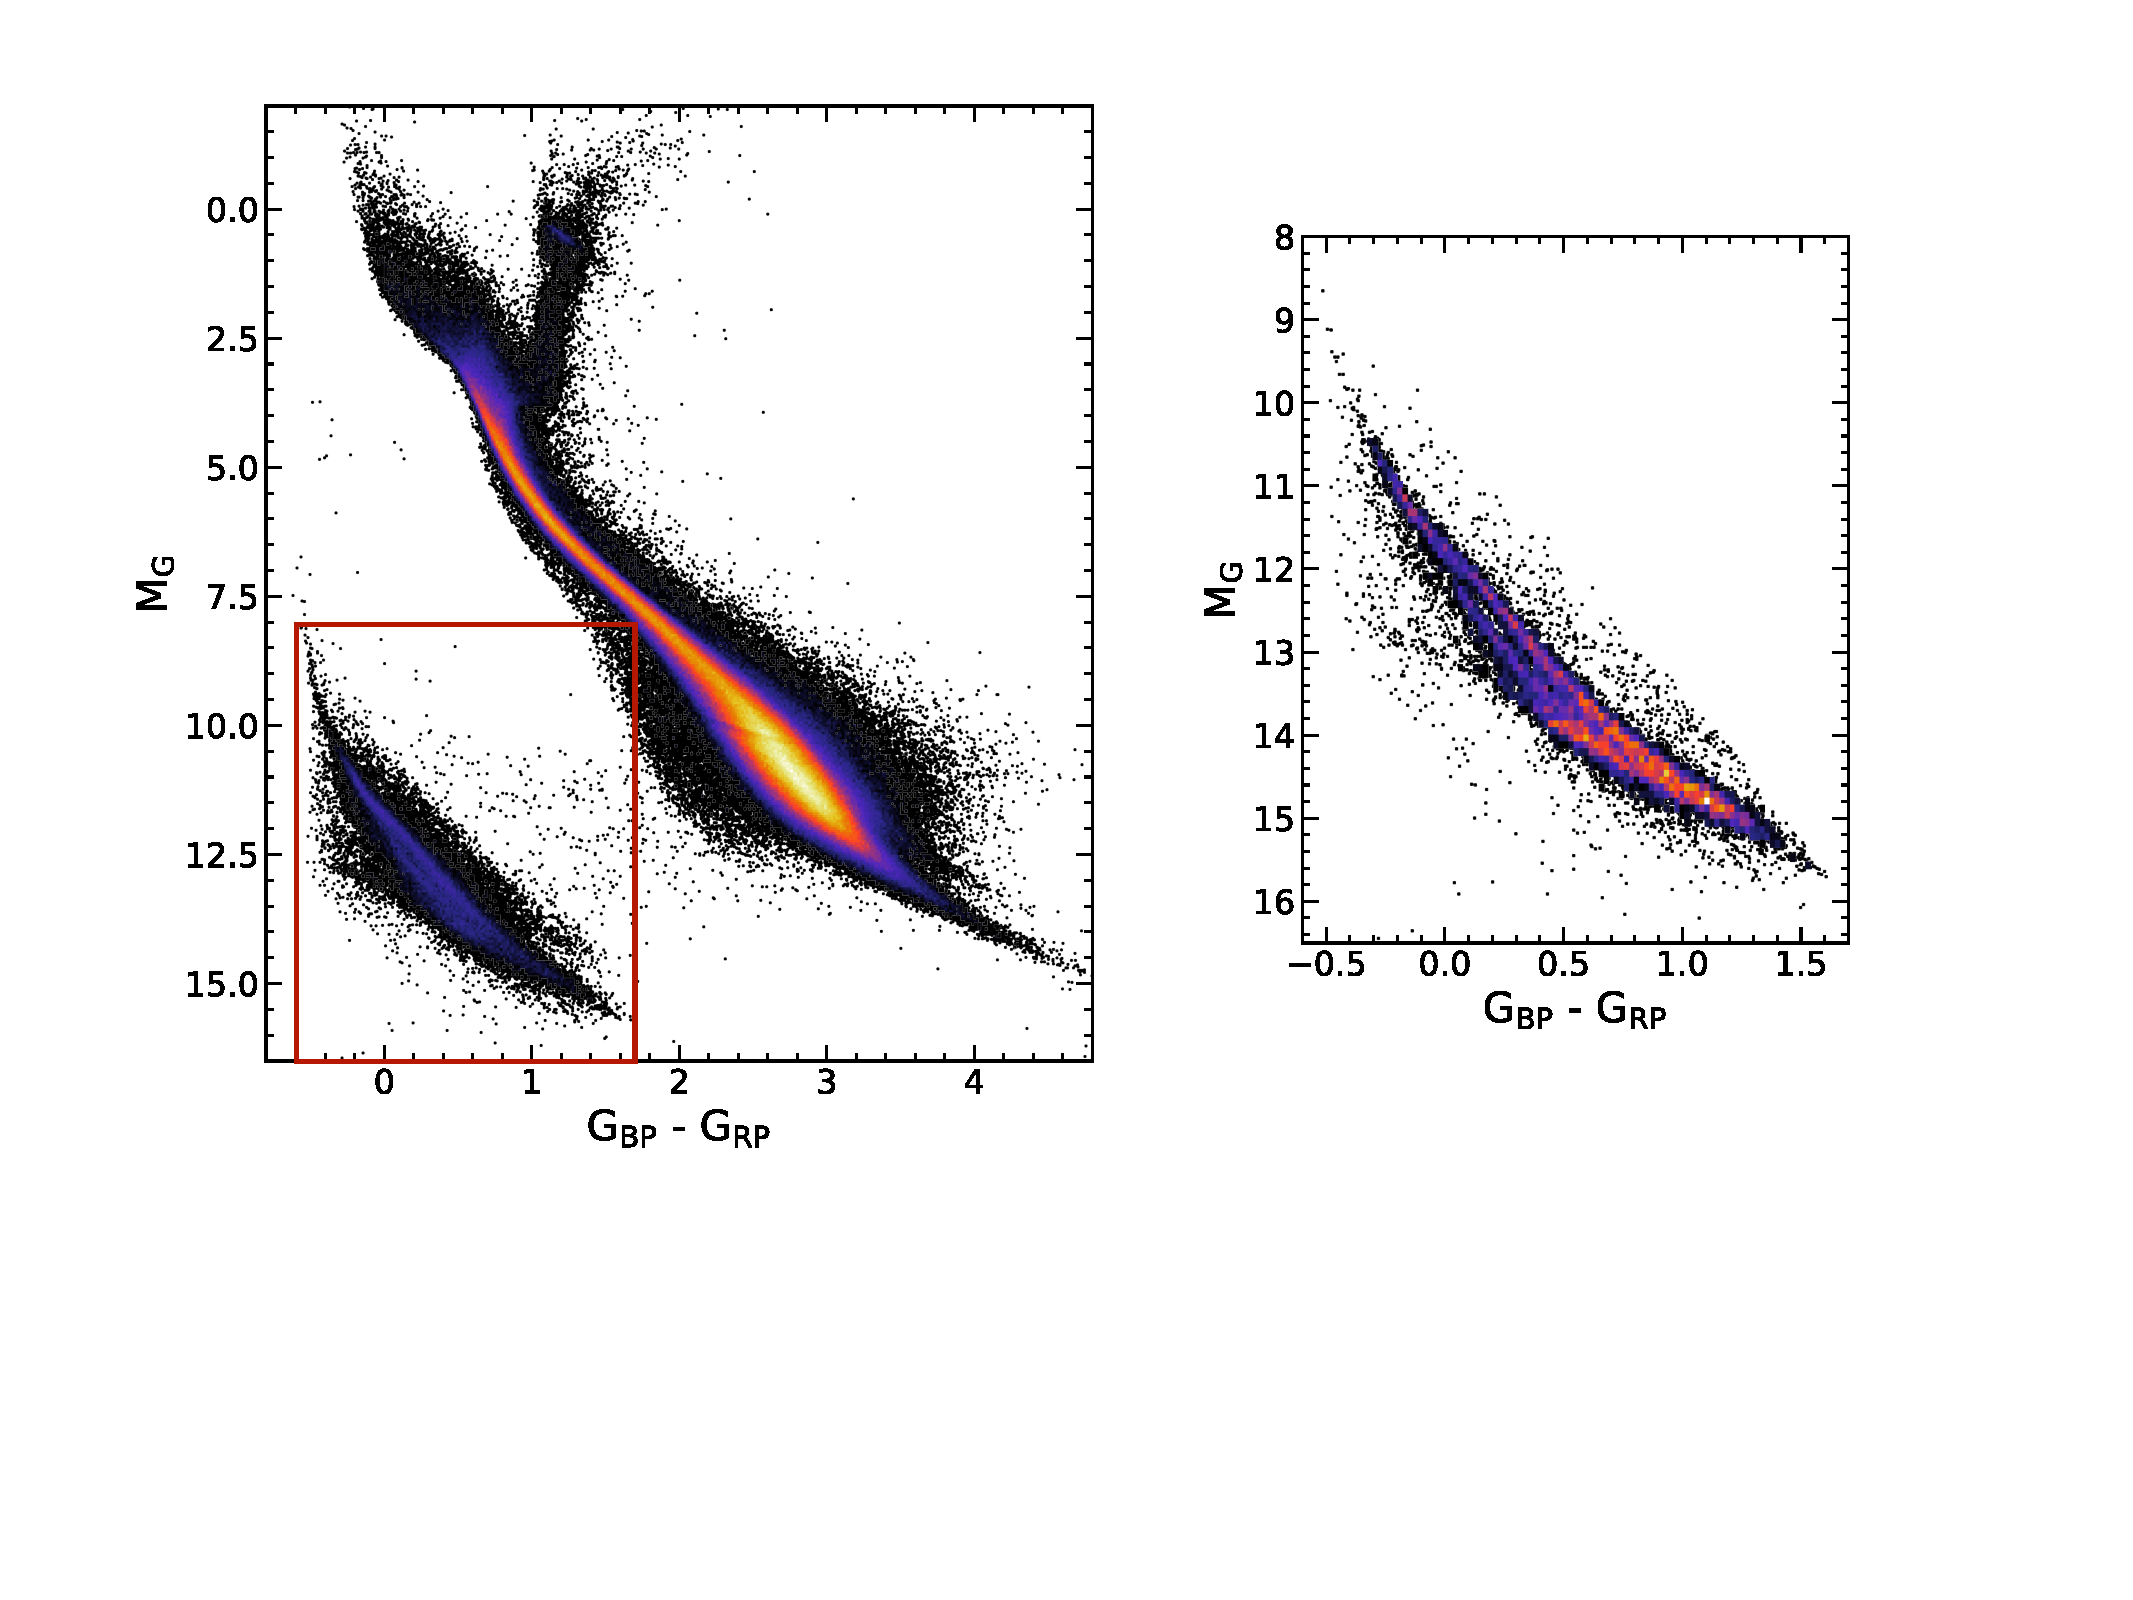
\includegraphics[width=0.95\textwidth]{images/gaiacmr.pdf}
    \caption{Colour-magnitude diagram of stars available as part of the Gaia data. Colour shows the square root of the number density. The left panel shows all stars in DR3 that are within 200 pc overlaid with a 500x500 histogram. The red box shows the WD region for which is then shown on the right in a similar style but for stars within 100pc and with increased bin width. A separation into two sequences can clearly be seen.} % Fig. 4.1
    \label{fig:cmd}
\end{figure}
Stars are sometimes called `nuclear foundries', as they fuse hydrogen into helium they create outward thermal pressure which upholds the star to gravitational pressure in hydrostatic equilibrium. The hydrogen is not infinite and eventually runs out and the star contracts, shedding its outer layers while the core begins fusing helium into heavier elements, creating a planetary nebular around it. For massive stars, the core is large enough that many heavier elements can start fusing but for stars between about $0.6-10\ \mathrm{M}_\odot$, at some point what is called electron degeneracy\footnote{Electron degeneracy pressure and more is explained in \cite{kippenhahn:12}} occurs and provides the necessary outward pressure. The star no longer fuses and all that is left is the core, a stellar `corpse' called a white dwarf is born. This is the fate of 97\% of all stars in the Milky Way \cite{fontaine:01}. The WD will live for a long time, but still cools slowly, growing fainter and redder over time which can be seen in the colour-magnitude diagram (CMD) of WDs, shown in Fig. \ref{fig:cmd}. The WD will be difficult to observe photometrically, as it is rather faint, and spectroscopically, due to the metals sinking below the observable photosphere as well as thermal broadening. 

Despite this, Gaia is able to observe quite a large number of WDs photometrically. In the Solar Neighbourhood (within 500 pc) we can, after some quality cuts, find about 130 000 WDs in EDR3. However, if we use an even closer sample limited to 100 pc, we can observe that the WD sequence is in fact not singular, but split into two. This result was first identified in \cite{dr2:hr} and has had two major suggestions put forth to explain it. Explanation \textbf{a)} suggests that the second sequence arises due to atmospheric differences in WDs. The upper, redder, sequence have hydrogen-dominated spectra (called DAs and constitutes {$\sim$}80\% of observed WDs) whereas the lower, bluer, sequence contains WDs with Helium (called DBs) or heavier elements dominating their atmospheres. We can refer to this simply as DAs or non-DAs for the purposes of Paper II. This explanation has shown to be able to explain the bifurcation very well in works like that of \cite{kilic:18, kilic:20} and \cite{gentile-fusilo:19}. Another recent discovery about the WDs is that their mass distribution is bimodal, with a main Gaussian centered on ${\sim}0.6\ \mathrm{M}_\odot$ and a secondary, smaller Gaussian around ${\sim}0.8\ \mathrm{M}_\odot$ (e.g., \citealt{elbadry:18, kilic:18, kilic:20}). This has lead to explanation \textbf{b)} that the second sequence could consists of heavier mass WDs, which have fainter and bluer cooling tracks. In single star evolution, the more massive WDs would come from more massive progenitors, which then become WDs much faster as well. For this reason they would have colder kinematics due to the age-dispersion relation \citep{aumer:16}. Mergers were suggested as a source of massive WDs but was ruled out by \cite{kilic:20} who failed to discover significant massive WDs with hot kinematics. Instead \cite{elbadry:18} shows that with the right choice of initial-final mass relation and continuous star formation, the second sequence can be populated by late-forming WDs. In summary, the second sequence can be explained as massive WDs formed recently. 

The two scenarios can be distinguished by their kinematics. The atmospheric composition should not have any bearing on the kinematics while, as explained above, the mass of WDs does. Therefore, we can investigate the kinematics of the two populations and try to provide insight into the bifurcation. 

\section{Inferring $f_v$}\label{sec:p2-inferring}
\begin{figure}[t]
    \centering
    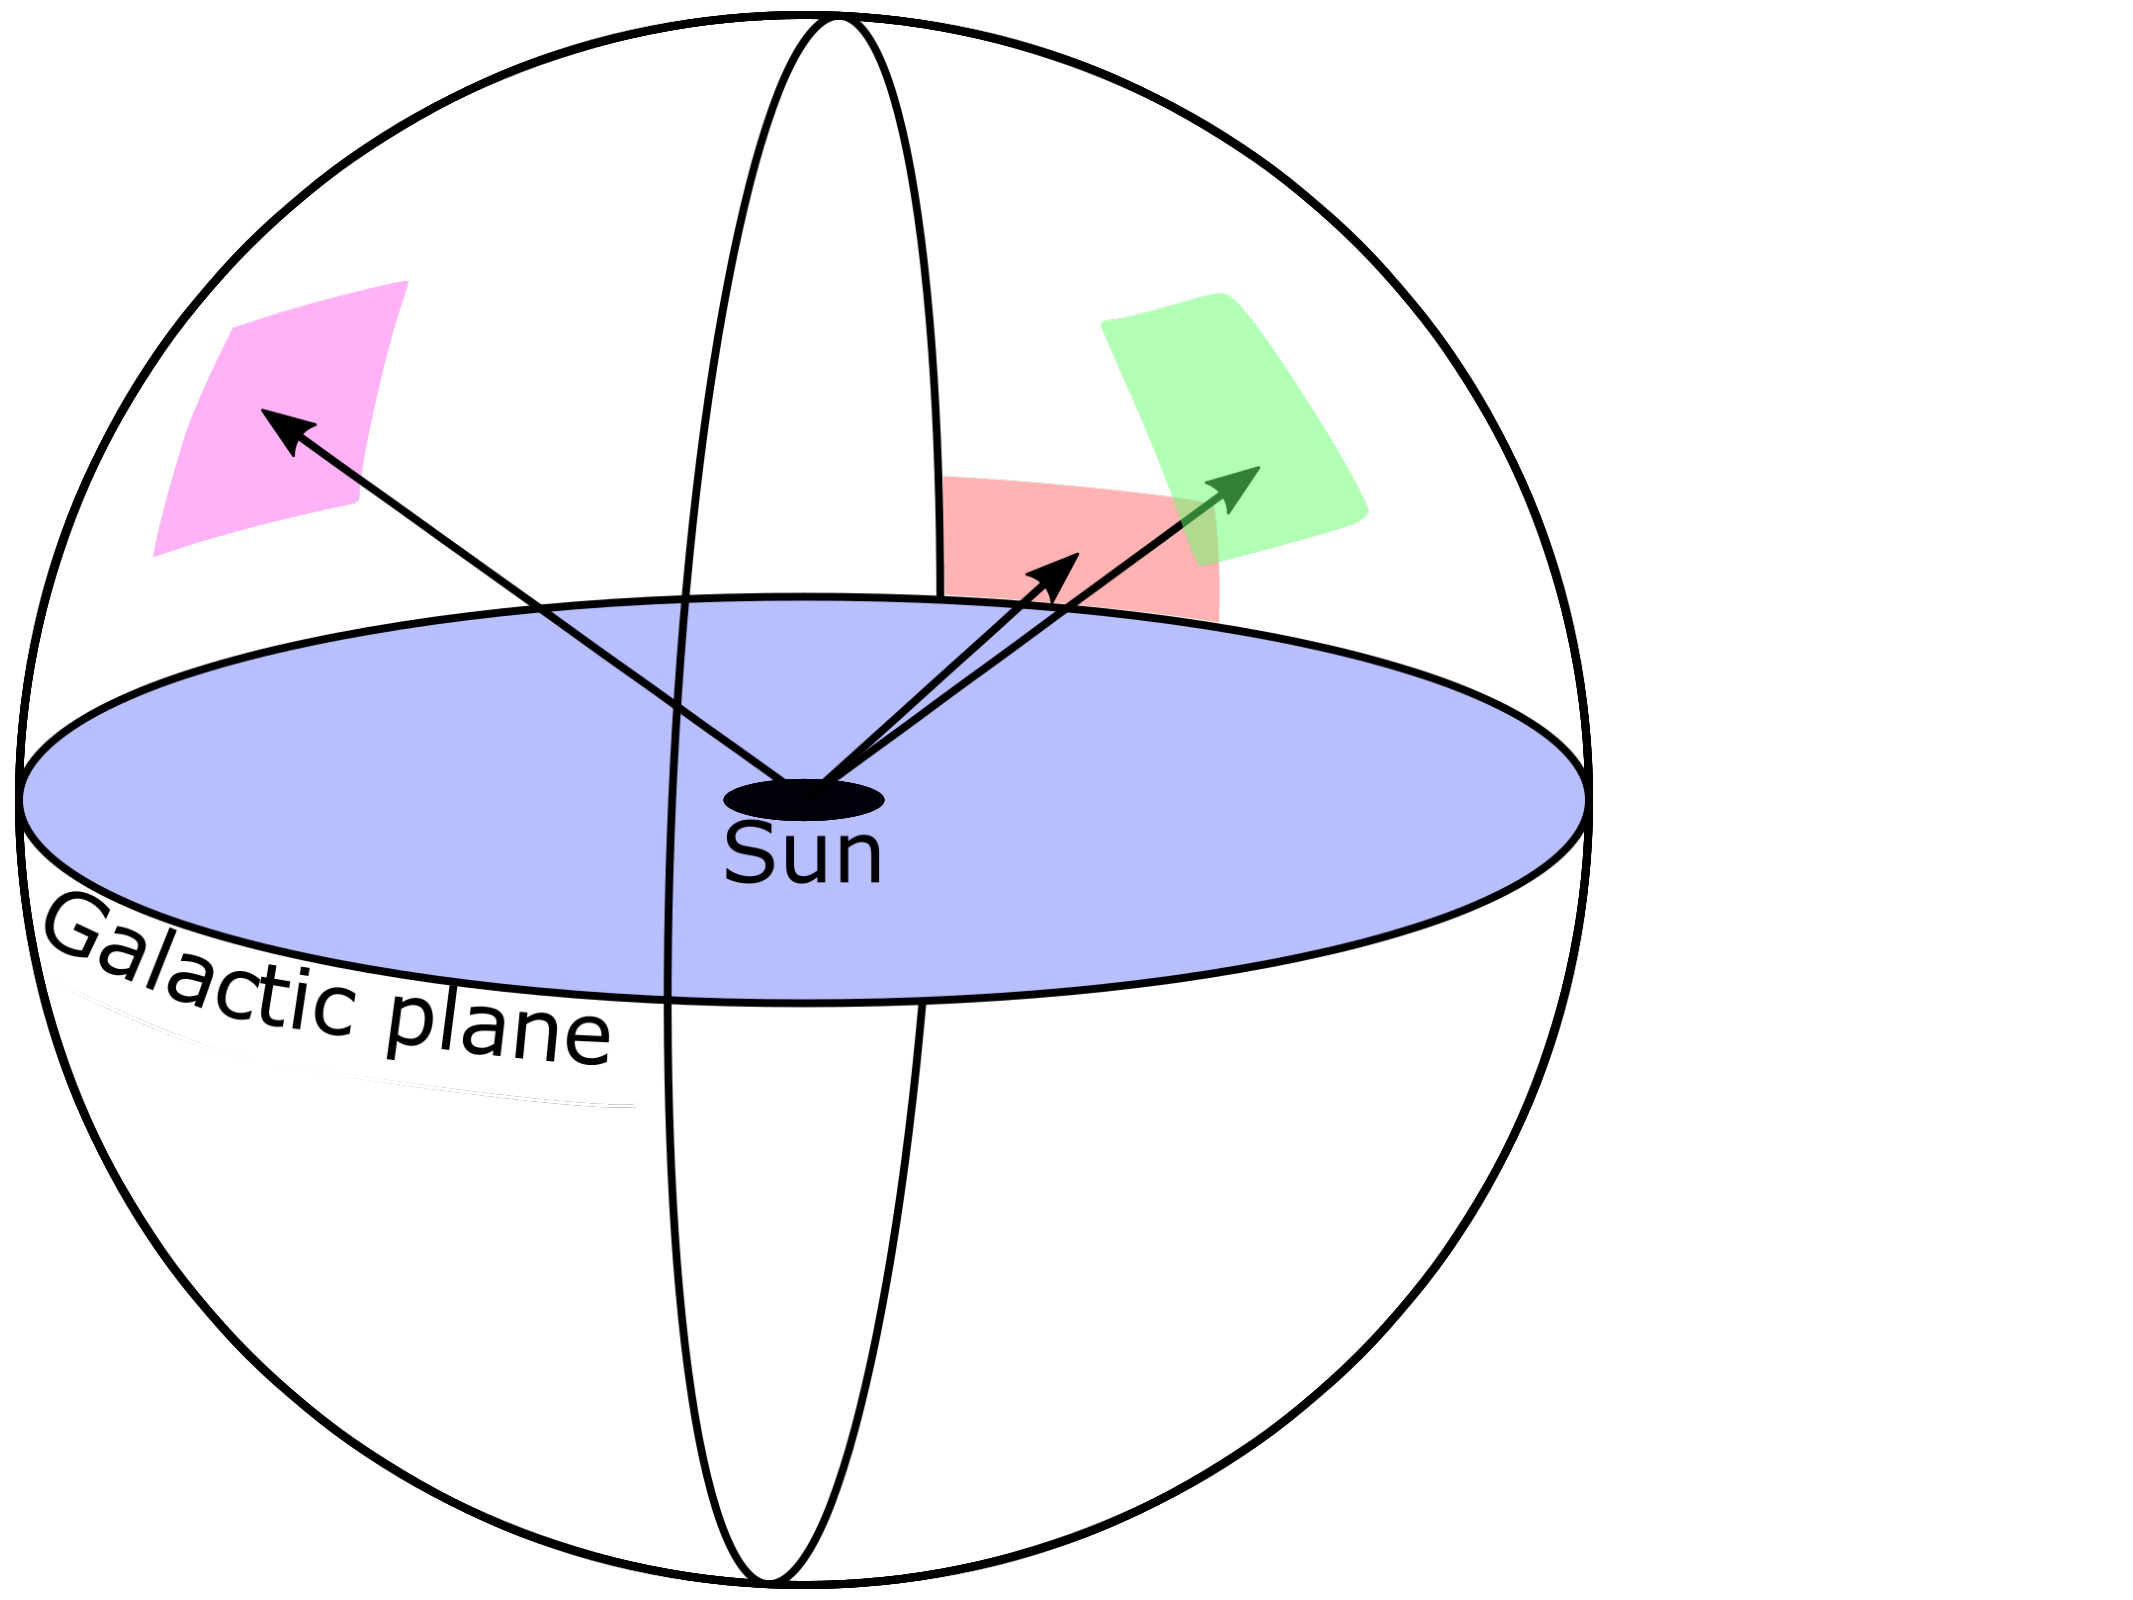
\includegraphics[width=0.45\textwidth]{images/projection.pdf}
    \caption{An illustration of positions on the celestial sphere from the point of view of a Solar system observer.} % Fig. 4.2
    \label{fig:projection}
\end{figure}
As shown in \cite{dehnen:98b}, the mean motion $\langle\pmb{v}\rangle$ and velocity dispersion $\pmb{\sigma}$ can be determined for a sample of stars given a few caveats. The on-sky positions have to be uncorrelated with the velocities, which means that we see the same velocities regardless of where on the sky we look. Consider the regions shown in Fig. \ref{fig:projection}. If there is a general mean motion for all parts of the sky, the line-of-sight motion of the red region will be given by the azimuthal component of tangential motion from either pink or green regions. Conversely, the azimuthal motion of stars in the red region will give the line-of-sight motion of the other two components. 

The same concept was used for the even more impressive feat of inferring the velocity distribution of Hipparcos stars in \cite{dehnen:98a}. We can write the probability distribution of tangential or transverse velocities in a given direction $\hat{\pmb{r}}$ as $\rho(\pmb{q|\hat{\pmb{r}}})$ where $\pmb{q}$ is the 2D vector of tangential velocities. To relate this distribution to the full velocity distribution we can write
\begin{equation}
    \rho(\pmb{q|\hat{\pmb{r}}}) = \int \mathrm{d}v_r f(\pmb{v}) = \int \mathrm{d}v_r f(\pmb{p} + v_r\hat{\pmb{r}}),
\end{equation}
where $\pmb{p}$ is the 3D projection of the tangential motion. The true distribution can of course not be determined using transverse motion alone but it can be estimated with a log-likelihood maximization of some model of it. We do this numerically by defining the velocity distribution to be
\begin{equation}
    f(\pmb{v}) = e^{\phi(\pmb{v})},
\end{equation}
where $\phi(\pmb{v})$ is given on a 3D velocity grid with $L_U\times L_V\times L_W$ cells with widths $h_U\times h_V\times h_W$. The final expression for the likelihood we seek to maximize, as a function of $\phi(\pmb{v})$, is:
\begin{equation}\label{eq:mple}
    \scalemath{0.8}{\tilde{\mathscr{Q}}_\alpha(\pmb{\phi}) = 
    \overbrace{N^{-1}\sum_{k} \ln \left[\sum_{\pmb{l}}e^{\phi_{\pmb{l}}}K(k|\pmb{l})\right]}^\text{\large Sum of PDF} - 
    \underbrace{\sum_{\pmb{l}}e^{\phi_{\pmb{l}}}}_\text{\large \hbox to 0cm{\hss Normalizing term \hss}} - 
    \overbrace{\frac{1}{2}\alpha h_xh_yh_z\sum_{\pmb{l}}\left(\sum_{\pmb{n}} \phi_{\pmb{n}}\Xi_{\pmb{n}\pmb{l}}\right)^2}^\text{\large penalizing term}.
    }
\end{equation}
Here, $N$ is the sample size, $\alpha$ is the smoothing parameter, $\Xi$ describes how the penalty relates to neighbouring cells, and $K(k|\pmb{l})$ is for each star $k$, the length of the line through each cell, $\pmb{l}$, formed by its tangential velocity and all possible radial velocities. 

To determine $\alpha$, we make use of the Gaia RVS. By selecting some reasonable range of test values for $\alpha$, we run the maximization on a corresponding sample of stars with measured radial velocities, in this case main-sequence stars. Since we know the velocity distribution of this sample, we can then choose the $\alpha$ that best reproduces the distribution of this calibration sample. Since the best choice of $\alpha$ depends on sample size, the calibration sample is picked so as to have about the same number of sources as the WD sample and uses an identical grid.

We chose a grid of $\pmb{n} = [100, 100, 72]$ cells with velocity ranges:
\begin{align*}
    U \in& [-150, 150]\ \mathrm{km\ s}^{-1} \\
    V \in& [-150, 50]\ \mathrm{km\ s}^{-1} \\
    W \in& [-80, 60]\ \mathrm{km\ s}^{-1},
\end{align*}
which provides a resolution of about $\Delta v = [3, 2, 2]\ \mathrm{km\ s}^{-1}$. The algorithm is also set up to use a so-called multigrid approach, where the solution is first found on a coarser grid which is interpolated and used as an initial guess for the maximization on a finer grid. This refinement occurs $3-5$ times depending on the grid size. 
\begin{figure}[t!]
    \centering
    \vspace{-40pt}
    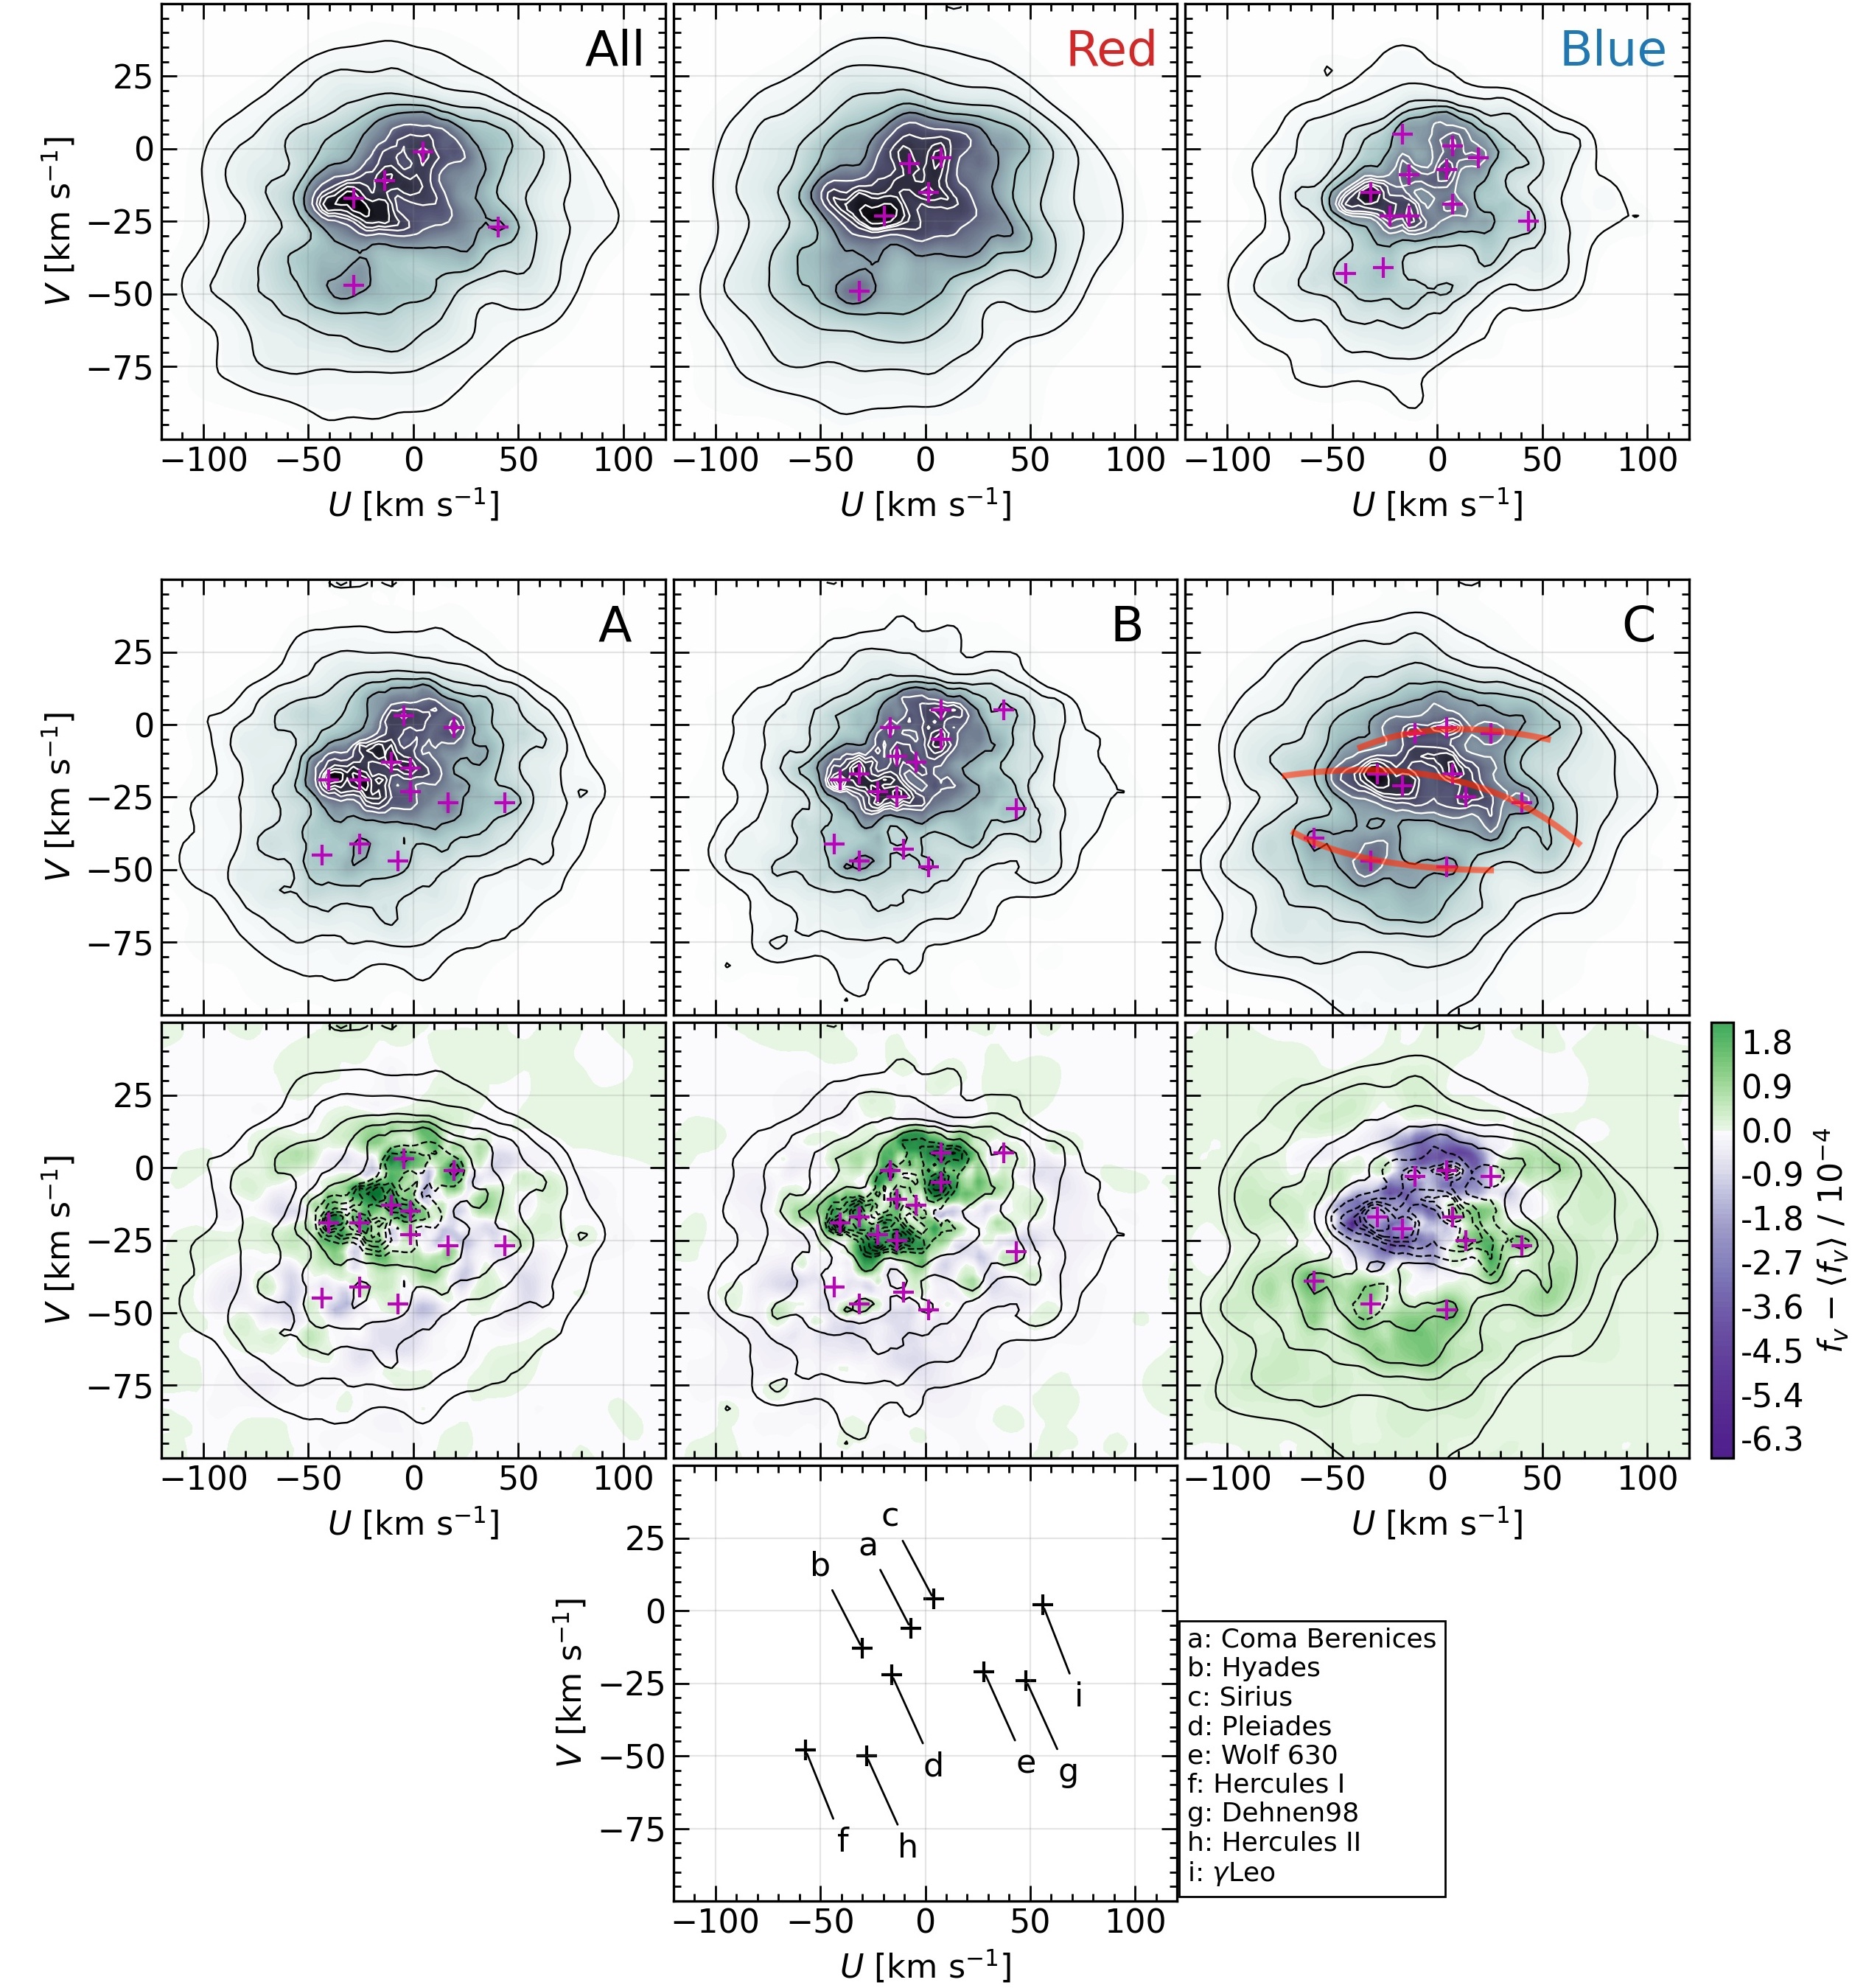
\includegraphics[width=1\textwidth]{images/wds_fv.jpg}
    \caption{Velocity distributions of the WDs in the $U-V$ plane. Purple crosses show identified features. Shown also are the different sub-samples with the top row showing the different bifurcated sequences, the middle row shows the magnitude bins mentioned in section \ref{sec:p2-inferring}. The bottom row shows the same magnitude bins subtracted by the mean of the three, to highlight where each bin is strongest or weakest. At the bottom is shown the first nine groups identified in \cite{antoja:12} for comparison.} % Fig. 4.2
    \label{fig:wd_fv}
\end{figure}
We split the WD sample by the bifurcation (between 12 and 14th magnitude where it is strongest) as well as into three equally sized magnitude bins, which we simply call \textit{A}, \textit{B}, and \textit{C} from brightest to faintest. The resulting velocity distributions in $U-V$ are seen in Fig. \ref{fig:wd_fv}. While the other velocity spaces are also available (and shown in the paper) the $U-V$ space shows the most structure. The overall shape can be quickly identified to match well with the known distribution of the main-sequence stars as seen in Fig. \ref{fig:veldist}. The magnitude bins can be seen increasing in velocity dispersion as they go from \textit{A} to \textit{C}, reflecting the age-dispersion relation. As the dispersion becomes larger, \textit{C} appears to have arch-like features as well, marked in the plot with red lines. The relative distributions on the third row has an unexpected result. We naturally would expect the more centrally fixated samples \textit{A} and \textit{B} to dominated close to the origin and \textit{C} would dominate further out. This is mostly the case apart from a small region around $(U, V) \approx (7, -19)\ \mathrm{km\ s}^{-1}$. The region does not match conclusively with any known moving group and only \cite{kushniruk:17} provides a nearby link to \textit{Coma Berenices} which has a suggested dynamical origin in \cite{monari:18}. 

The bifurcated regions are seen in the top row and show similar dynamical features. However, the velocity dispersion of the red sample is clearly larger than the blue. This hints of hotter kinematics and as such, we look to the dispersion of the samples rather than the full distribution for further analysis. 
\section{Two kinematic populations}\label{sec:p2-populations}
\begin{figure}[t]
    \centering
    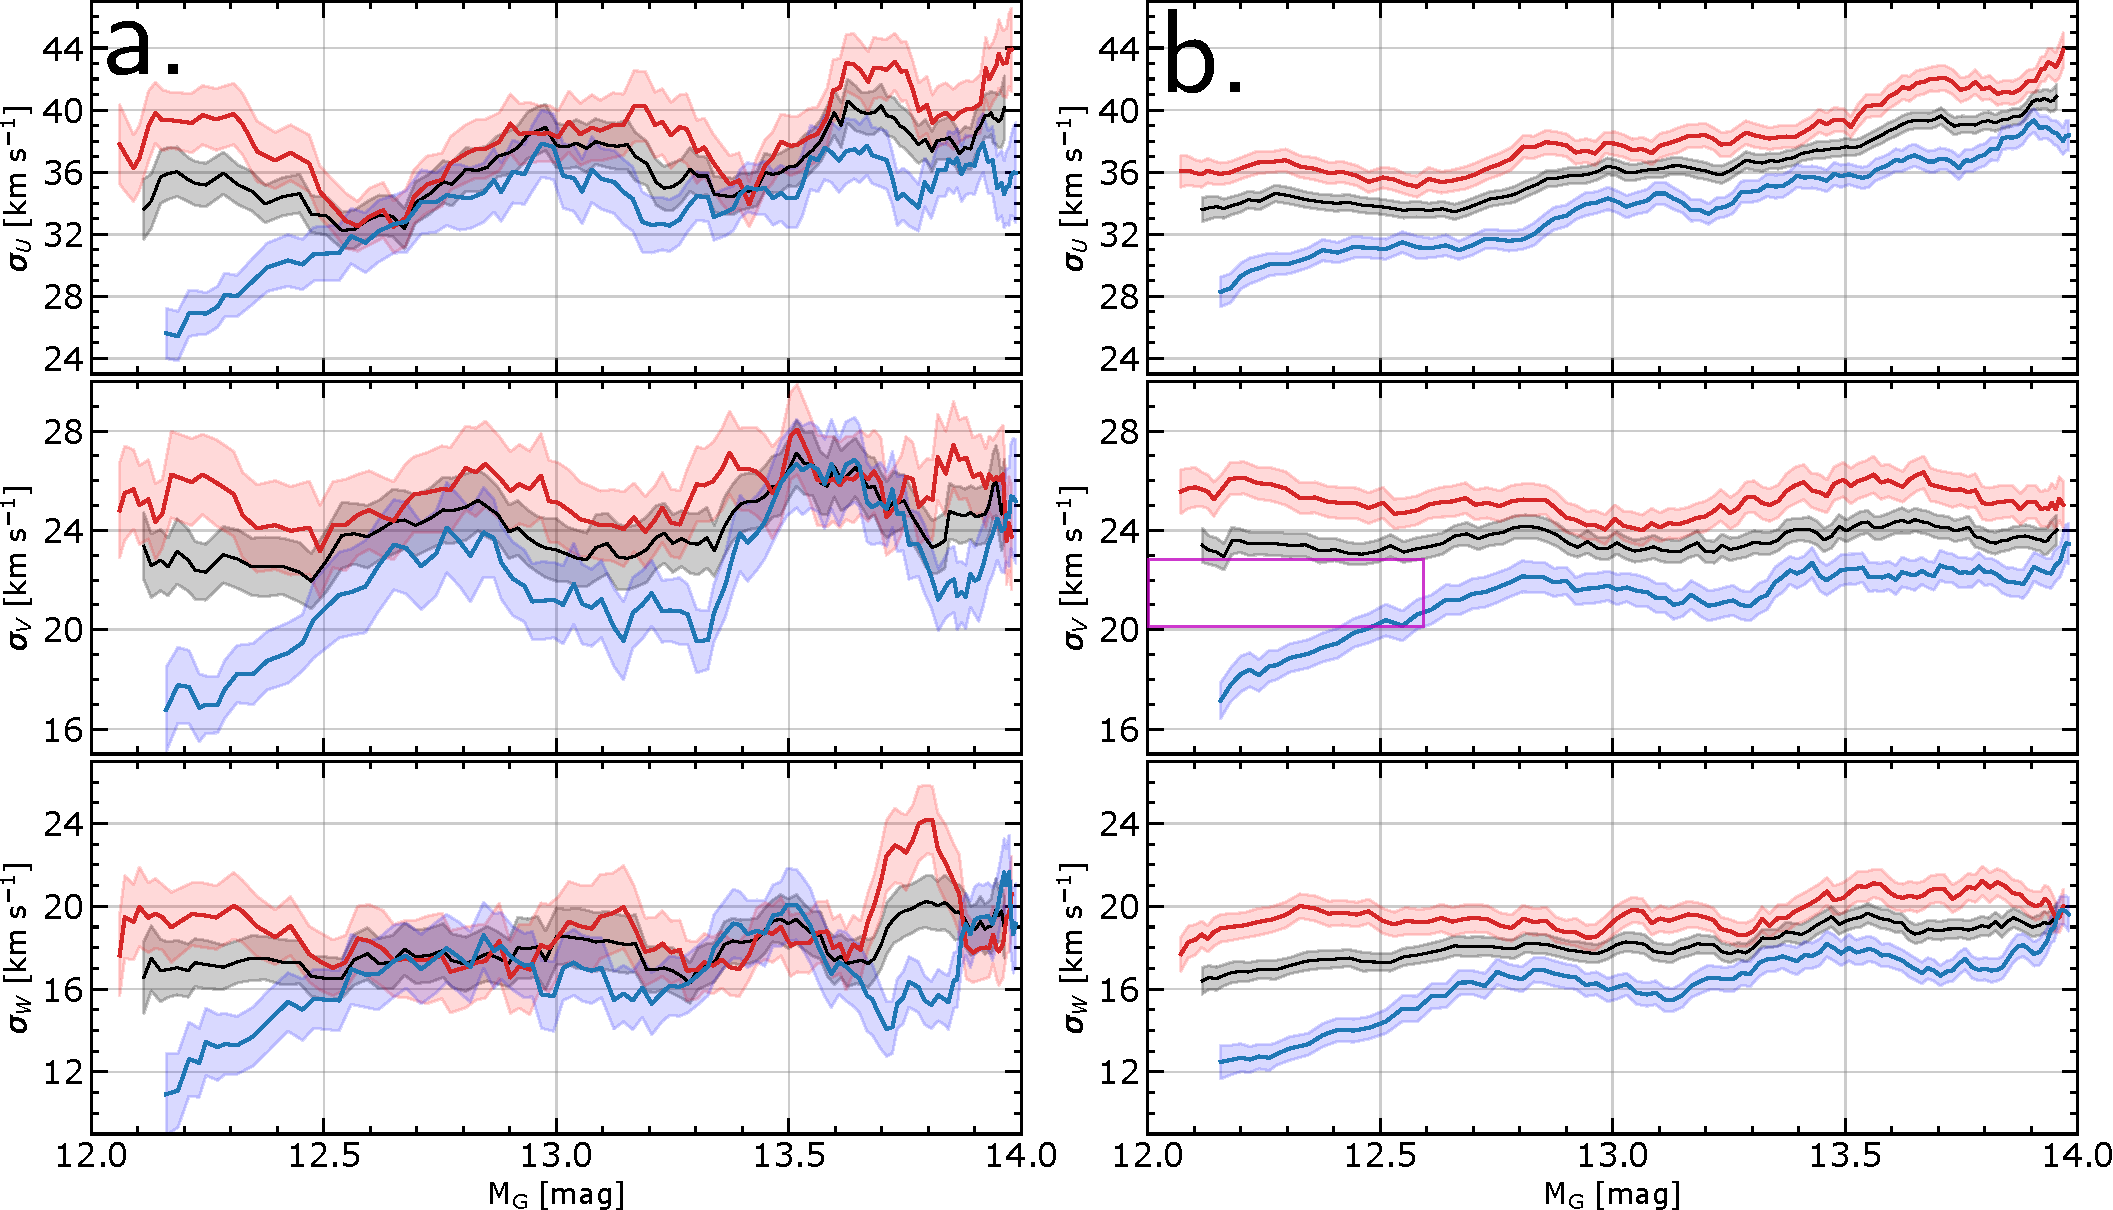
\includegraphics[width=1\textwidth]{images/moving_dispersion.pdf}
    \caption{Moving velocity dispersion calculated in the three directions of $U$, $V$, and $W$, for the bifurcated sequences between 12th and 14th magnitude where they are visible. \textit{a.} shows the moving dispersion for the red and blue sequences as well as the joint sample using WDs which are closer than 100 pc. The shaded regions show the 1$\sigma$ uncertainty regions. \textit{b.} same as the a. but for WDs up to 200 pc. Both plots show clearly a separation between the red and blue samples and when the 200 pc sample is used, they barely even overlap within 1$\sigma$.} % Fig. 4.3
    \label{fig:moving_disp}
\end{figure}
We use the same method as in \cite{dehnen:98b} to determine the velocity distribution for a sample of stars. But we also employ a moving window across the visible bifurcation to better compare the sequences as they cool. The velocity distributions in Fig. \ref{fig:wd_fv} used WDs within 500 pc, whereas here we use WDs limited to either 100 pc or 200 pc, the result of which can be seen in Fig. \ref{fig:moving_disp}. Here it can be clearly seen for the 200 pc sample that the red sequence has larger kinematics across all magnitudes. For the 100 pc sample this is also visible but less so. We can however show that the two samples are drawn from the same underlying distribution. We determine the $Q$-statistic for the two dispersion of the samples at various points: 
\begin{equation}
    Q = \frac{\sigma_{d_1} - \sigma_{d_2}}{\sqrt{\Delta \sigma_{d_1}^2 + \Delta \sigma_{d_2}^2}},
\end{equation}
where $d_1$ is the 100 pc sample and $d_2$ are stars between 100-200 pc. Both the red and blue Cumulative Distribution Functions (CDF) matches well with a Gaussian distribution, and using a Kolmogorov-Smirnov test gives $P$-values between them and a true Gaussian which all lie above 0.8. Therefore, the difference between the two figures is simply statistical noise. 

This shows that the two sequences between magnitudes 12 and 14 are \textit{kinematically separate and distinct populations}. In regards to the discussion in section \ref{sec:p2-whitedwarfs}, this would agree well with the two sequences being comprised of different masses where the heavier mass WDs are formed recently, giving them less time to be heated dynamically and thus forming the blue sample we have seen here. It cannot be ruled out the atmospheric composition is partly responsible for the bifurcation in the CMD but it cannot be the sole explanation. In our 100 pc samples, we cross-matched with the Montreal White Dwarf Database \citep{dufour:17} to find that 85\% of the cross-matched red sample and 39\% of the blue are DAs, so there are undoubtedly non-DAs in the second sequence. If they truly correspond to 60\%, they still do not significantly alter the kinematics of the sample as a whole. It can be argued that the crystallization of massive WDs would provide massive WDs which are still visible in our range due to cooling delays (e.g., \citealt{tremblay:19, bergeron:19, bauer:20}). If this were the case, these massive WDs would have had the necessary time to dynamically heat. If this process is contaminating the sample, the fact that we still see the kinematic split is arguably even more significant.

Further insight into the bifurcation of the WD sequence will likely require a combination of studied both spectroscopic and kinematic. Here, we have demonstrated the possibilities of working with only proper motions when analysing the vastness of the Gaia data. 
\chapter{Paper III}\label{chap:paper3}
\section{Introduction}\label{sec:p3-intro}
Following on from the previous paper, we wished to apply our implemented MPLE on other interesting subsamples of the \textit{Gaia} data. We were also able to make use of the improved Gaia DR3. 

The study of kinematic space has a division in it between the Galactic disc and the stellar halo. This division guides our choice of samples and is understandable since the two regions are affected by different dynamical processes. The disc we have already described in section \ref{sec:p2-intro}. The stellar halo on the other hand, is where the evidence of past mergers between the Galaxy and its neighbours will be found \citep{helmi:20}, which can, for example, contribute to the velocity distribution and cause enhanced star formation \citep{ruiz-lara:20}. This is what inspires our chosen samples of data: the Solar neighbourhood disc sample and a the stellar halo.

Since our method lets us utilise the astrometry only, we can then achieve some impressive sets of data for these populations. Limiting the Solar neighbourhood to $\varpi > 5$ mas (or 200 pc) we can use as many as 1 171 846 stars, after having applied all of our quality cuts. This is comparable to current results using the Gaia RVS like \cite{lucchini:22} which has 982 879 stars in the Solar neighbourhood. However, they do not apply any quality filters on photometry or astrometry, apart from a criteria of 20\% parallax uncertainty $(\varpi / \sigma_\varpi > 5)$. We restrict our results to only 10\% uncertainty and if we were to use 20\%, we would have 3 592 434 sources before applying our quality filters, which highlights the benefits of our method.

For the stellar halo, a recent similar sample is \cite{dodd:22} which limits their halo to 2.5 kpc as well as imposing a velocity cut whereby the motions of the star with respect to the Local Standard of Rest (LSR) must be greater than 210 km/s. Since the circular speed at the position of the sun is ${\sim}$233 km s$^{-1}$ \citep{mcmillan:17}, this cut removes the vast majority of the disc stars. Our cuts are slightly more generous with a distance limit of 3 kpc and velocity limit of at least 200 km s$^{-1}$, albeit on transverse velocity rather than full space velocity. Their sample contains 72 274 stars, whereas ours contains 456 273. 

We use these two samples to estimate their velocity distributions. For the Solar neighbourhood, this is done in the same manner as for the WDs in the previous paper. The stellar halo distribution is inferred in spherical coordinates instead, since it is more spherical in shape around Galaxy. We also divide the stellar halo into \textit{in situ} and \textit{accreted} components (e.g., \citealt{naidu:20}). The velocity distributions are studied closely to determine what known structure is apparent and what new structure we are able to identify. Some novel structures do appear in our analysis, specifically in the accreted halo where we find two new features that we call \textit{MMH-1} and \textit{MMH-2}.
\section{Gaia's view of the local Galaxy}\label{sec:p3-gaiaview}
\begin{figure}[t]
    \centering
    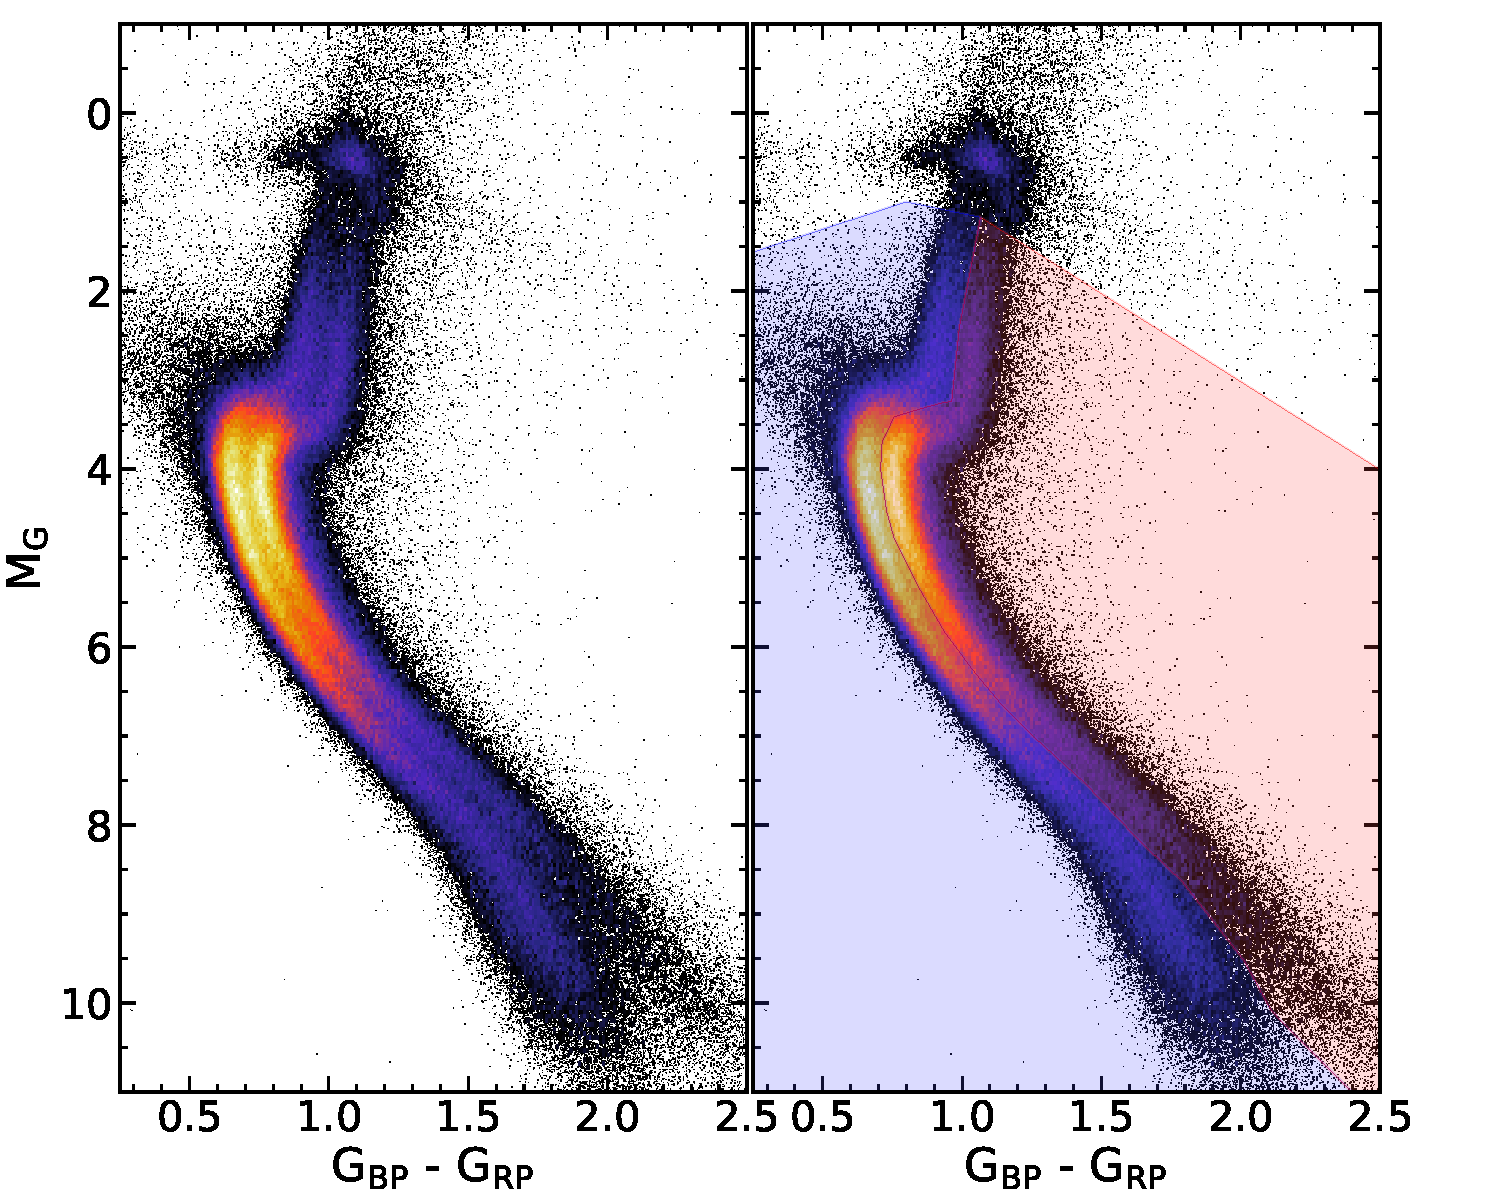
\includegraphics[width=0.75\textwidth]{images/GES_cmd.pdf}
    \caption{Colour-magnitude diagram of our filtered halo sample. Colour shows the number density. Right panel shows selected regions for the left and right sequences overlaid with shaded areas.} % Fig. 5.1
    \label{fig:halo_cmd}
\end{figure}
\begin{figure}[t]
    \centering
    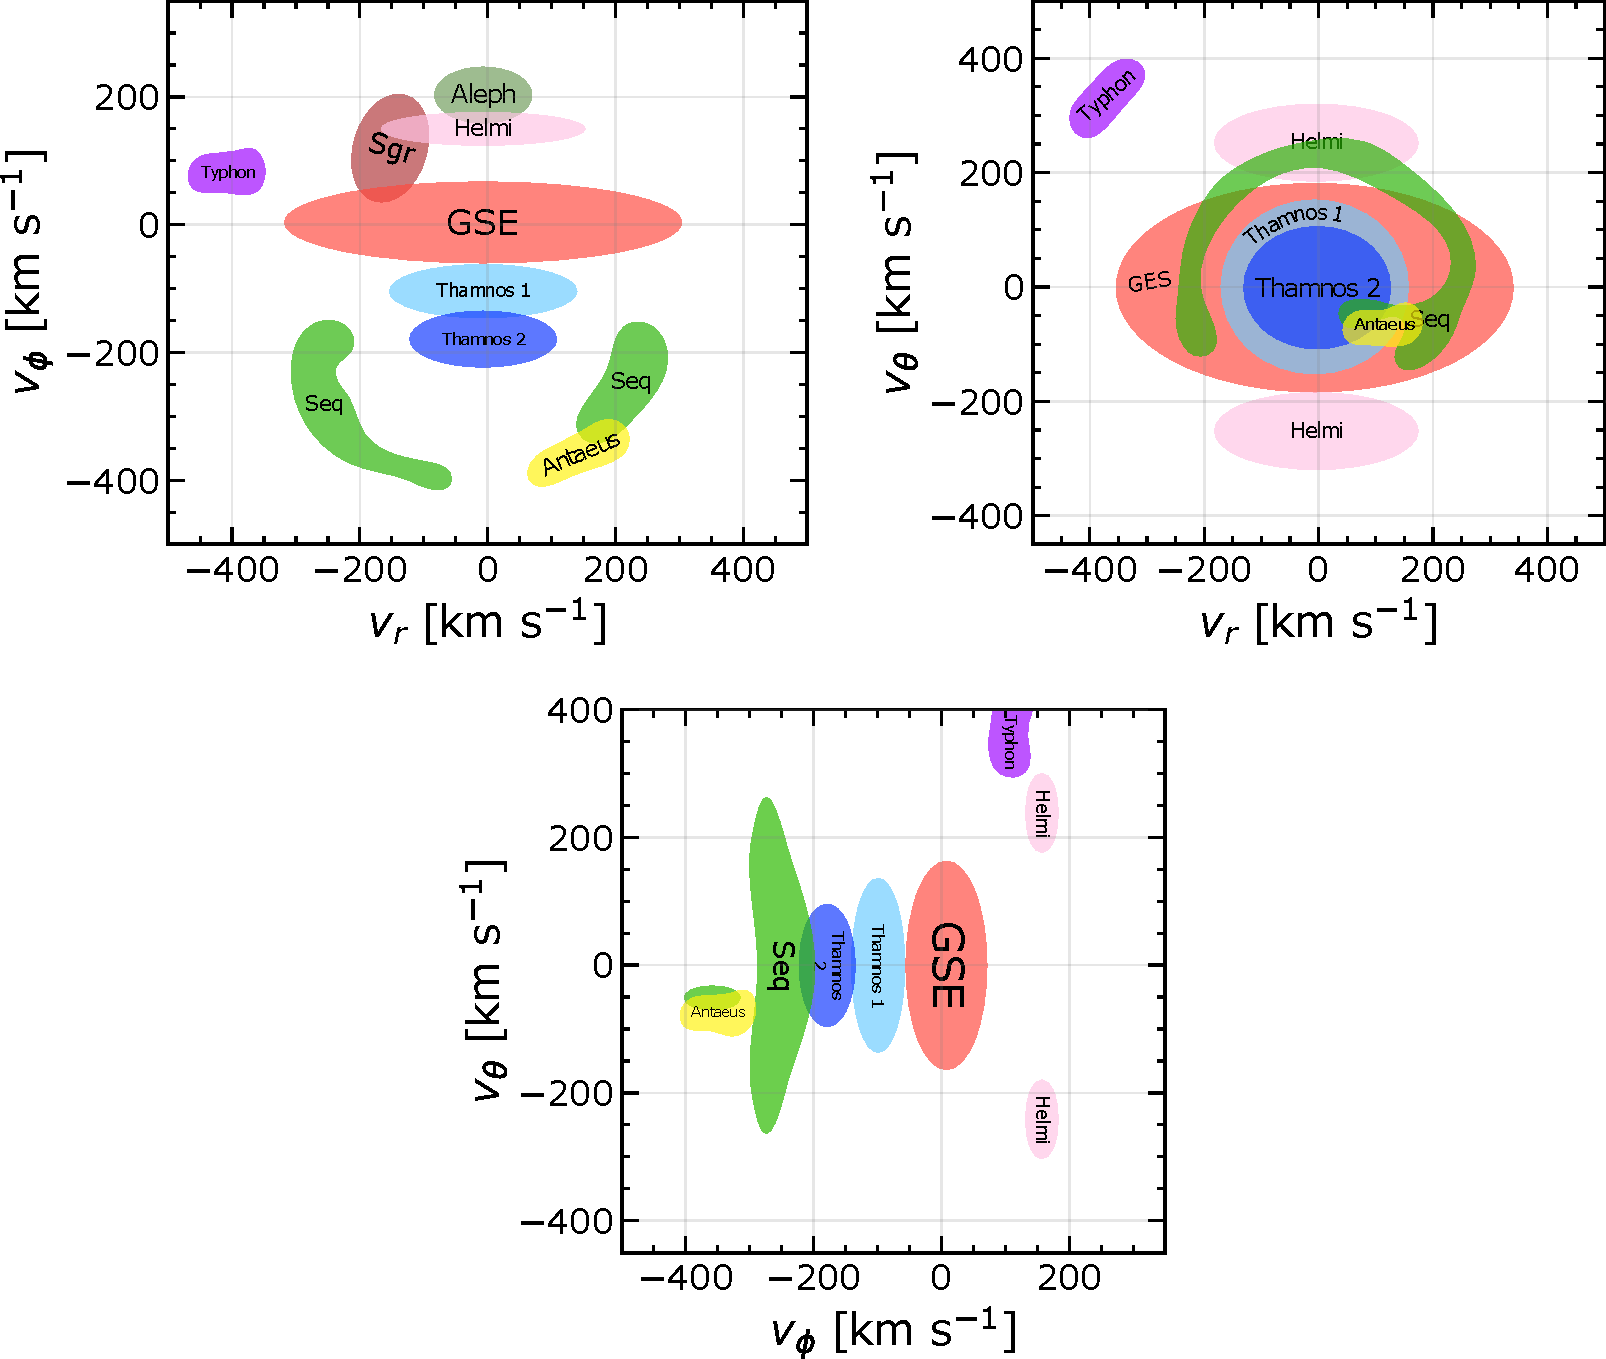
\includegraphics[width=0.85\textwidth]{images/map_only_b.pdf}
    \caption{Estimated typical positions of known velocity structures in the stellar halo. Figures show the velocity spaces of $(v_r, v_\phi)$ (top left), $(v_r, v_\theta)$ (top right), and $(v_\phi, v_\theta$ (bottom). Here $v_r$ points outwards from the Galactic centre, $v_phi$ increases in the direction of Galactic rotation, and $v_\theta$ increases from south to north Galactic poles.} % Fig. 5.2
    \label{fig:halo_map}
\end{figure}
There has been plenty of work done to try and characterise the velocity substructure that exists in the disc and stellar halo. We briefly discussed the Solar neighbourhood in chapter \ref{chap:paper2} and showed several moving groups from \cite{antoja:12} in Fig. \ref{fig:wd_fv}. We briefly mentioned \cite{lucchini:22} above which is one of the more recent works that investigates the disc structure. The current picture of the local disc velocity distribution is one with multiple arch-like structures, of which many fractured individual substructures can be identified (see e.g., Table 1 from \citealt{lucchini:22}). 

For the stellar halo, things look slightly different. This is currently a very active field, but some smaller discoveries were made already 20 years ago using Hipparcos to identify the Helmi streams \citep{helmi:99}. It is, perhaps, not surprising that \textit{Gaia} has had a significant impact upon this field as well. When DR2 was released, two important findings came soon thereafter. The first was in the colour-magnitude diagram of the stars with large transverse velocities. By selecting stars with $v_T > 200$ km s$^{-1}$ \cite{dr2:hr} showed that there were two separate main sequences, a finding that we recreate and show in Fig. \ref{fig:halo_cmd}. The left sequence was then found to be connected to an accretion event from a single object \citep{belokurov:18, koppelman:18} which is called \textit{Gaia-Sausage-Enceladus} or \textit{GSE}, which was the second finding. This lead to a successful hunt for other accreted populations in the stellar halo. At the time of writing, some of the larger discovered structures include \textit{Sequoia} \citep{myeong:19}, \textit{Antaeus} \citep{oria:22}, \textit{Thamnos} 1 and 2 \citep{koppelman:19}, and \textit{Typhon} \citep{tenachi:22}, to name a few. We show the expected positions of these features as well as some smaller ones in Fig. \ref{fig:halo_map}. This puts into perspective how structured the Galactic stellar halo has been revealed to be with the use of \textit{Gaia} data.

Since we have access to the most expansive catalogue of sources from \textit{Gaia}, we aim to expand the view of substructure in the local parts of the Galaxy's disc and stellar halo.

\section{Structures: The old and the new}\label{sec:p3-structures}
\begin{figure}[t!]
    \centering
    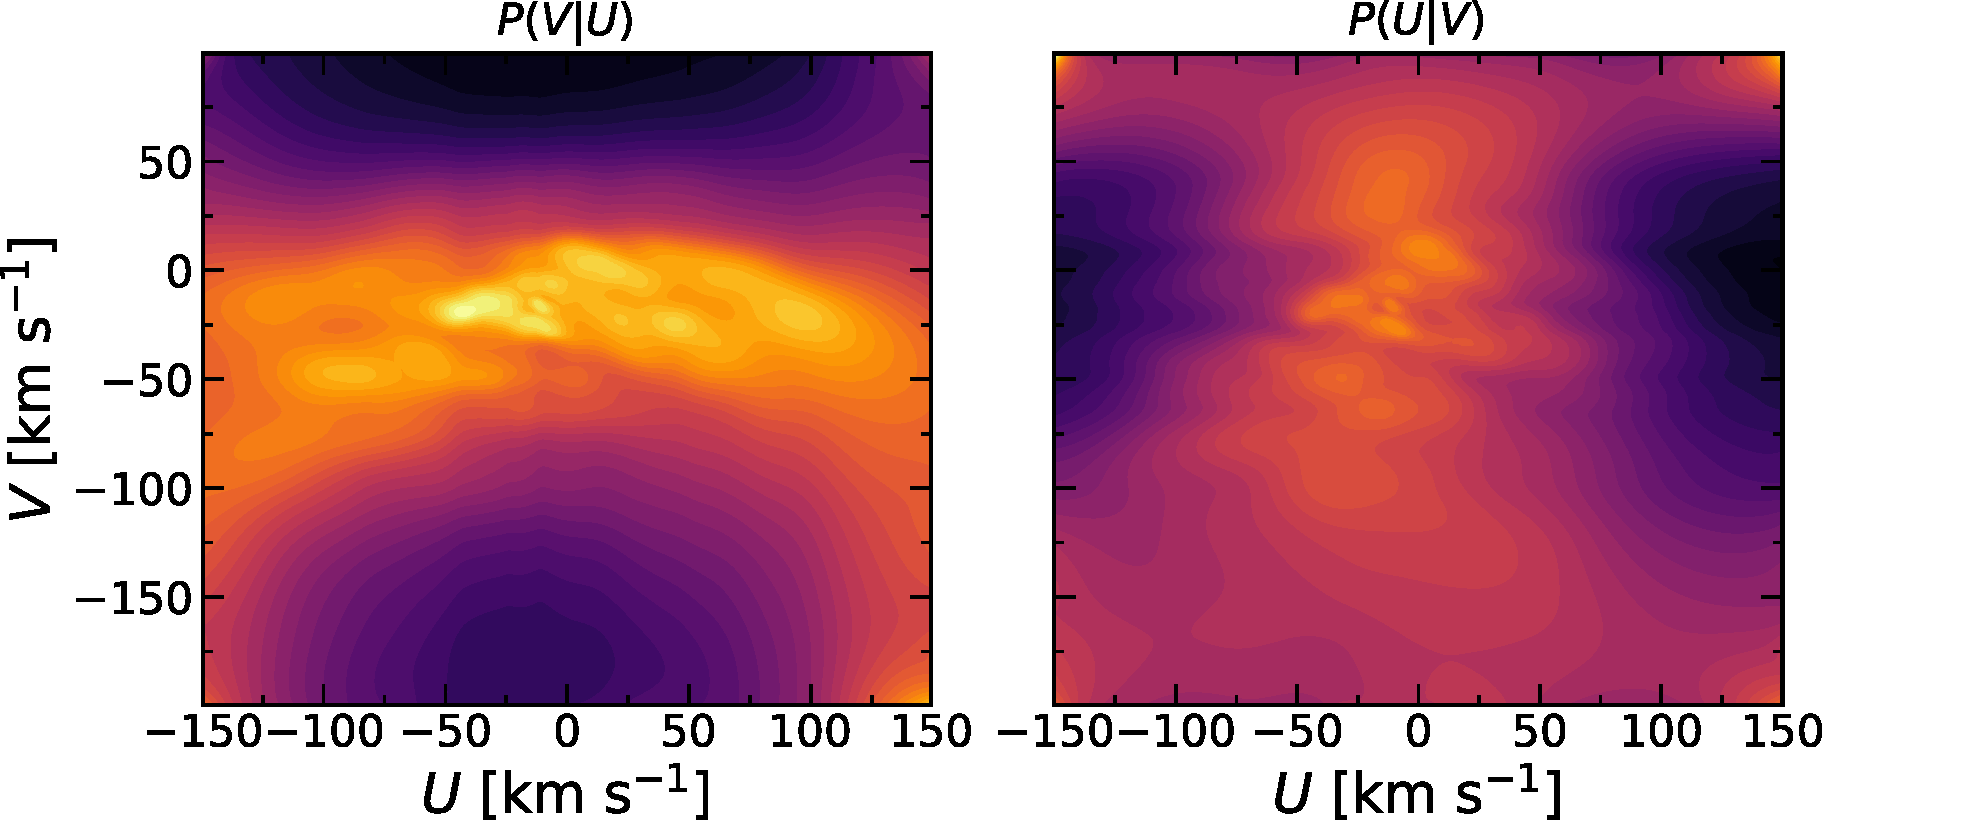
\includegraphics[width=0.9\textwidth]{images/conditional_snbh.pdf}
    \caption{The conditional probability of one velocity component in $(U, V)$ against the other. Left shows $P(V|U)$ and right shows $P(U|V)$ which reveals rich substructure beyond the central dominating groups. The color scaling shows the density such that $P(v)^{0.25}$.} % Fig. 5.3
    \label{fig:cond_snbh}
\end{figure}
\begin{figure}[t!]
    \centering
    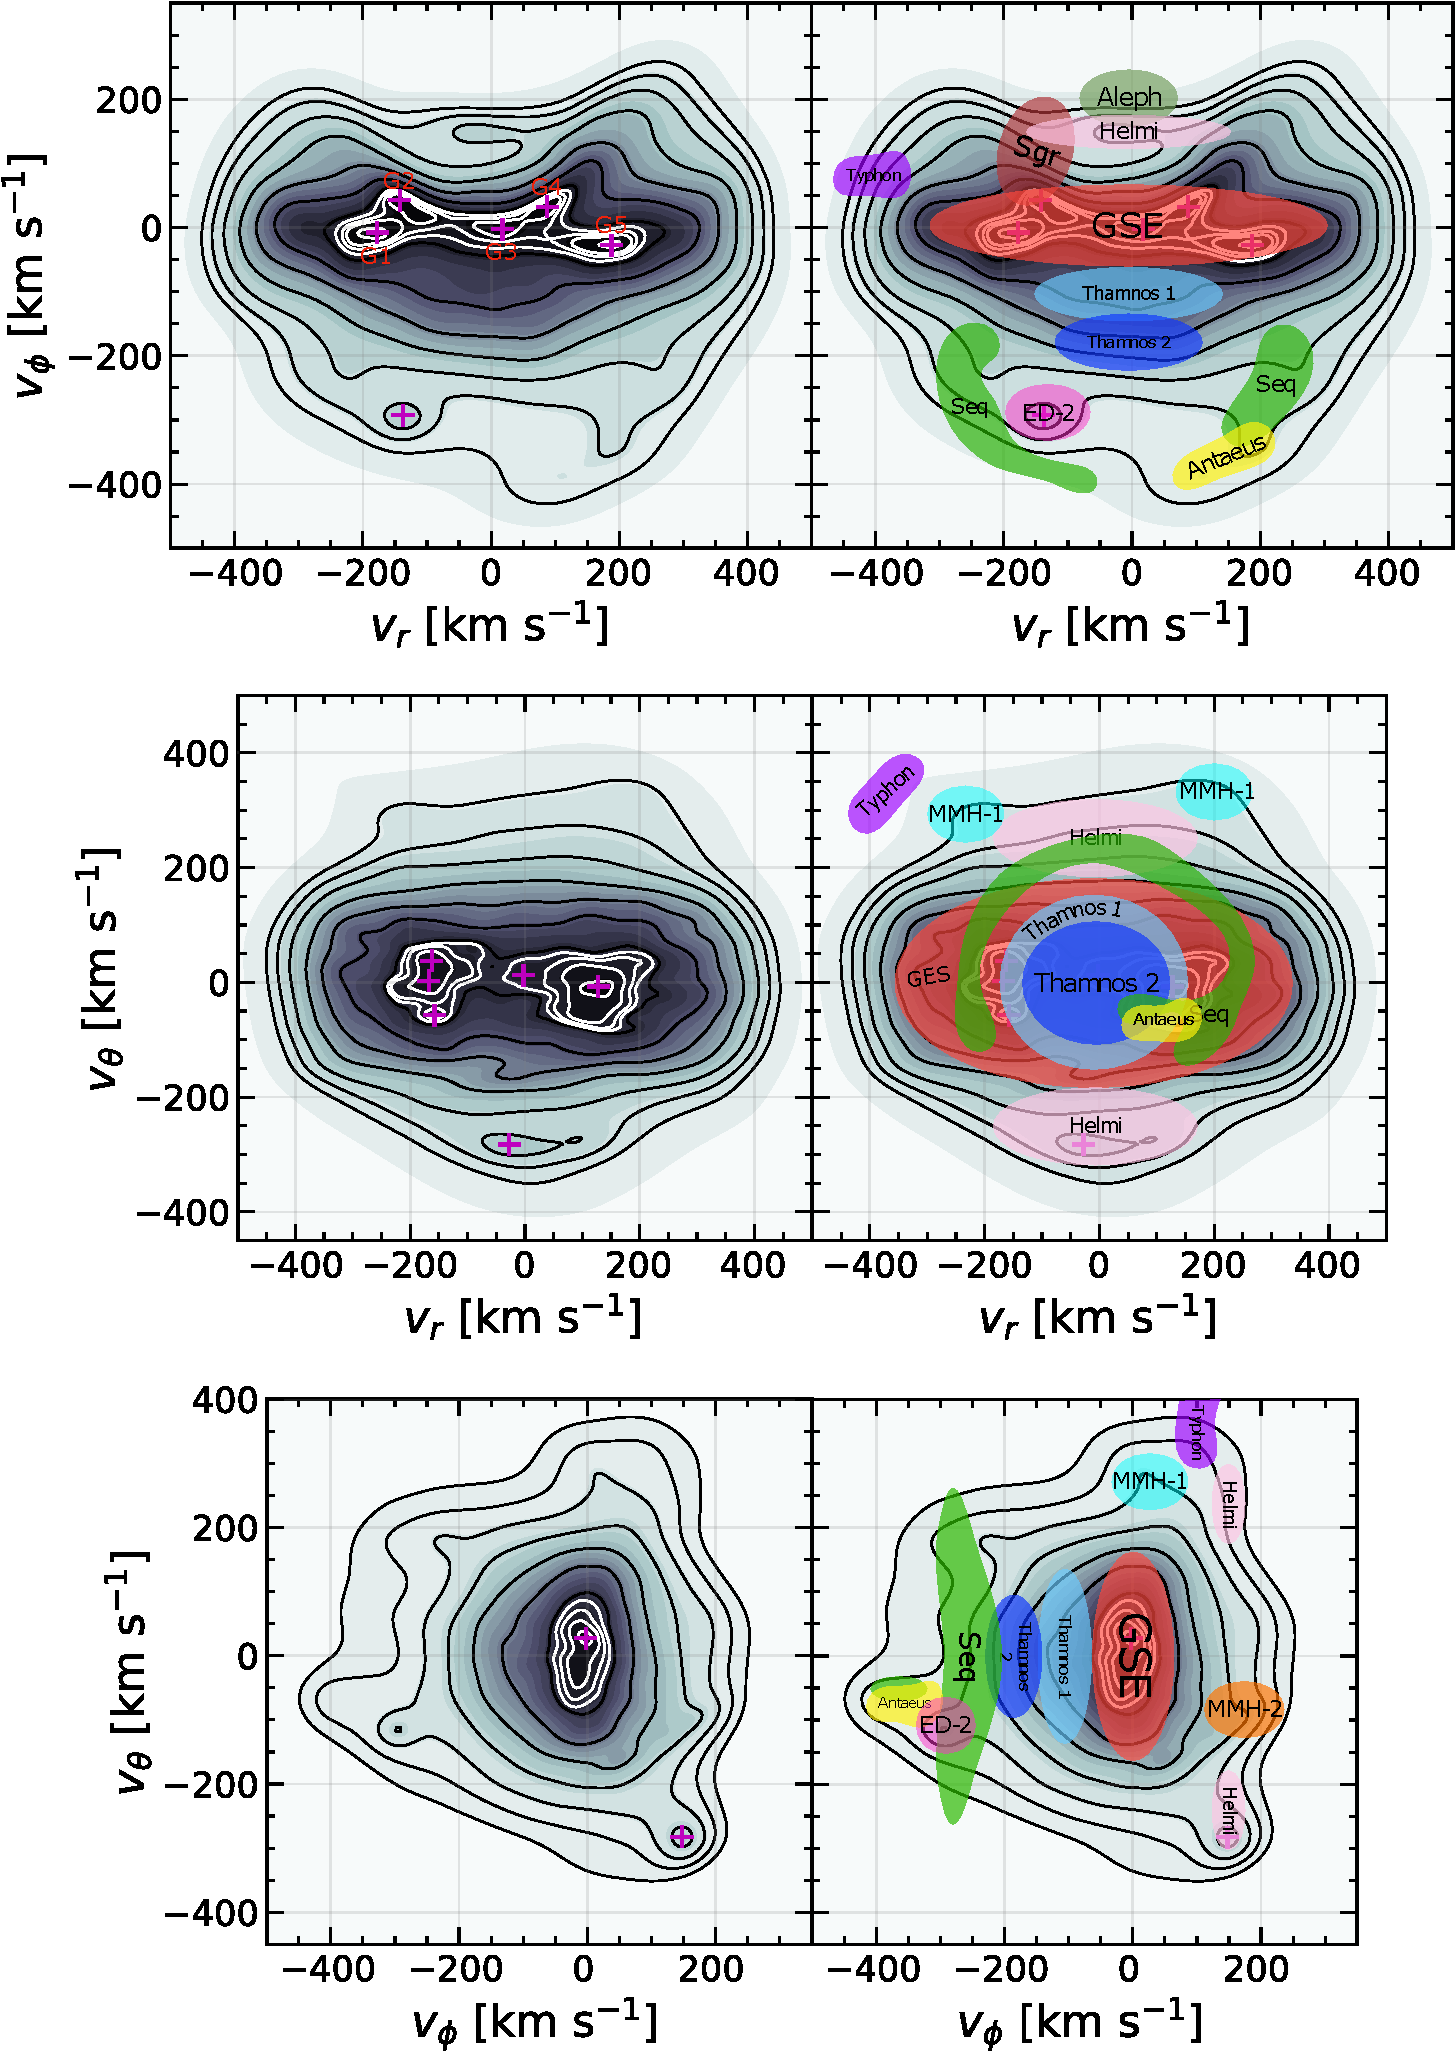
\includegraphics[width=0.8\textwidth]{images/halo_fv.pdf}
    \caption{Velocity distributions of our left halo sample in $(v_r, v_\phi)$ (top row), $(v_r, v_\theta)$ (middle row), and $(v_\phi, v_\theta$ (bottom row). Right right column shows the same distributions overlaid with the positions of expected substructure from literature, in a similar style to what is done in \cite{naidu:20} and \cite{mardini:2022}. Significant peaks are marked with purple crosses and in the top left figure five significant groups belonging to the \textit{GSE} are marked as G1-G5.} % Fig. 5.4
    \label{fig:halo_fv}
\end{figure}
\begin{figure}[t!]
    \centering
    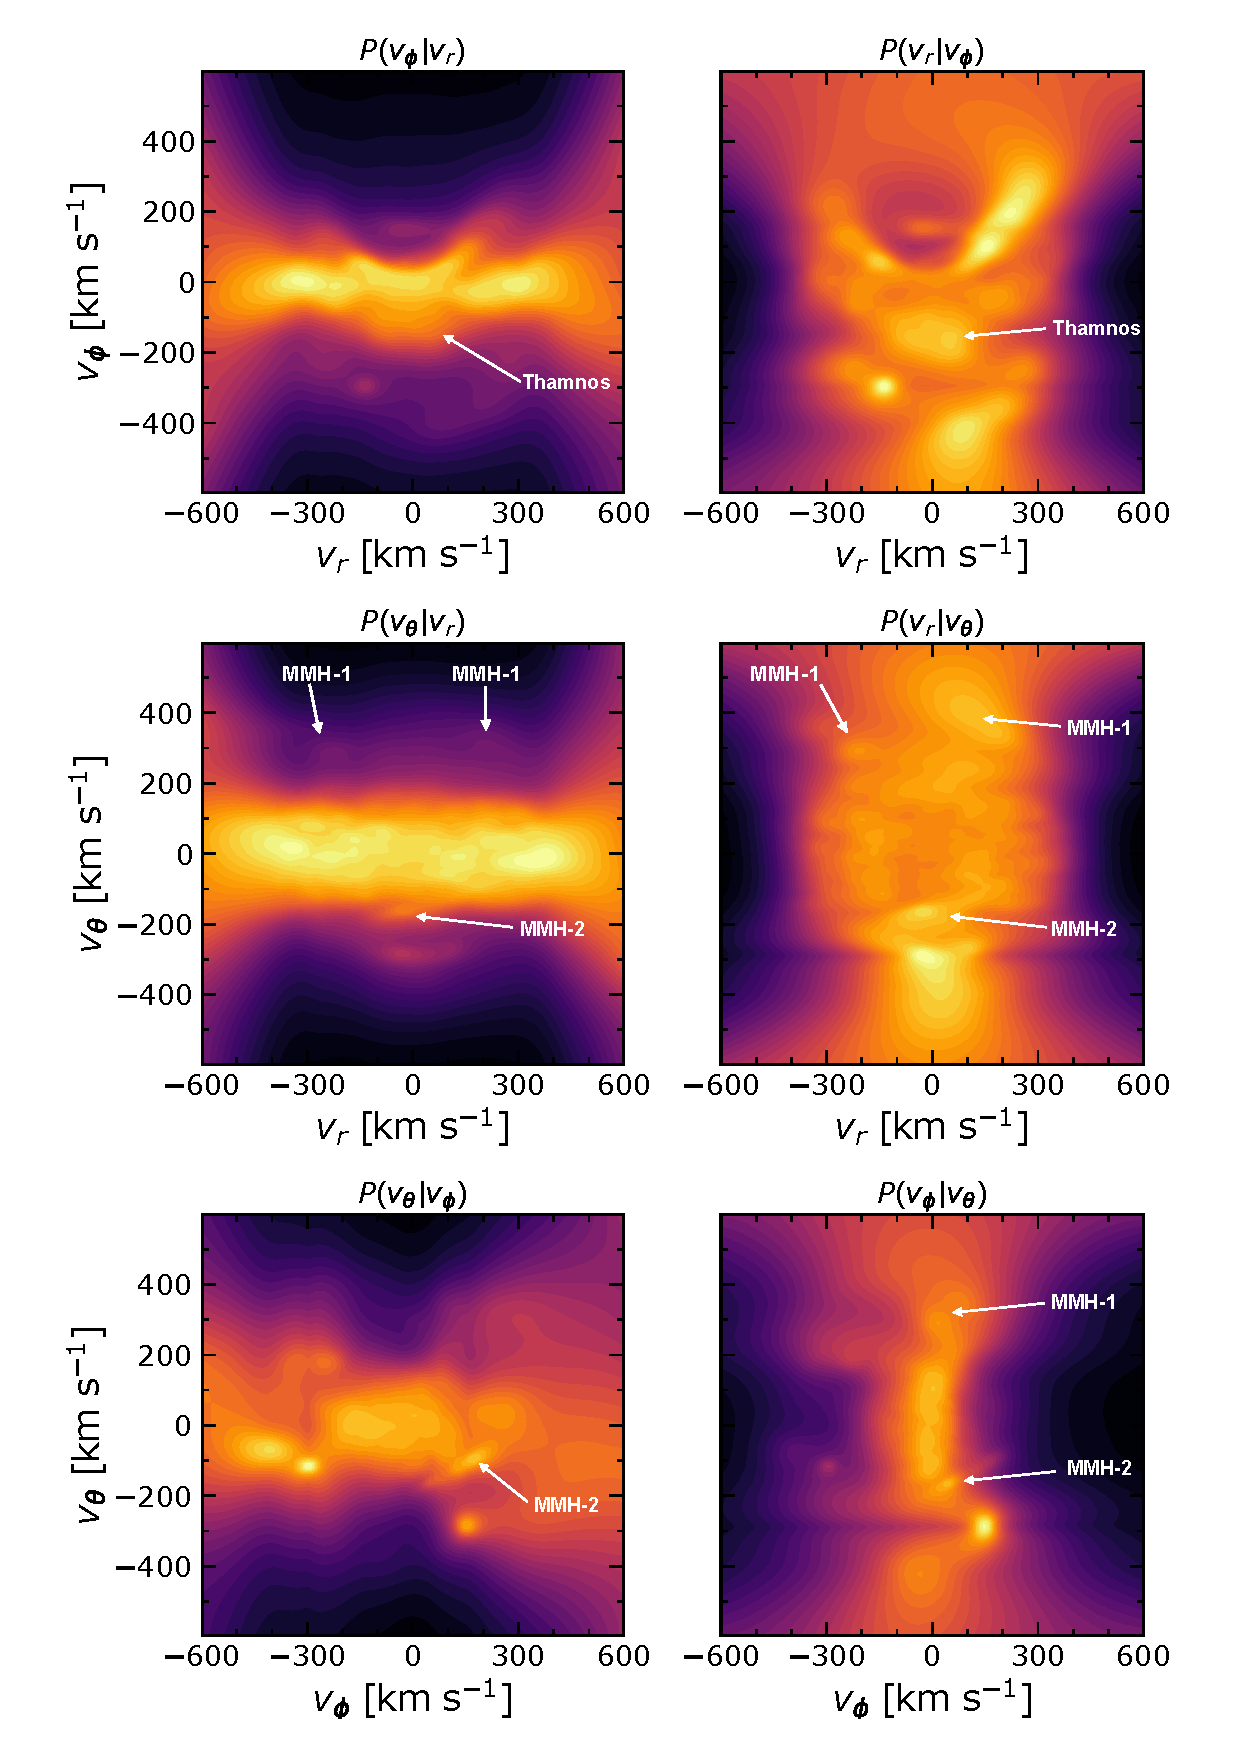
\includegraphics[width=0.8\textwidth]{images/conditional_halo.pdf}
    \caption{Conditional probability distributions of the velocities from Fig. \ref{fig:halo_fv} with the left column showing the conditional probability distribution of the $y$-axis velocity on the $x$-axis velocity. The right column shows the inverted conditional probabilities. Density is scaled such that $P(v)^{0.25}$.} % Fig. 5.5
    \label{fig:cond_halo}
\end{figure}
When we investigated the velocity distribution of the Solar neighbourhood using our sample we found that the distribution is heavily dominated by the typical major moving groups: \textit{Sirius}, \textit{Coma Berencies}, \textit{Hyades}, \textit{Pleiades}, and \textit{Hercules}. The distributions also contains weaker traces of \textit{Dehnen98} and \textit{Wolf630}. Since the distribution is so heavily dominated by these features, a better way of viewing hidden structures comes in the form of conditional probabilites. For the $(U, V)$ plane where most of the known structure exists, this means that we calculate $P(V|U) = P(U,V) / P(U)$ and $P(U|V) = P(U,V) / P(V)$. The result is probability maps that can reveal structure that is otherwise blotted out by the major groups and we show this in Fig. \ref{fig:cond_snbh}. Here can be seen much richer structure like $\epsilon$\textit{Ind} (e.g., \citealt{antoja:12, kushniruk:17, bobylev:16}) at $(U, V) = (-100, -50)$ km s$^{-1}$, \textit{Dehnen98} \citep{antoja:12} at $(U, V) = (50, -30)$ km s$^{-1}$, and likely \textit{Antoja12} from e.g. \cite{kushniruk:17} at $(U, V) = (100, -30)$ km s$^{-1}$. The conditional probability is clearly a useful tool for the outer regions.

The velocity distributions of the two halo samples were produced and as expected, the right sequence shows very little accreted structure and a such we placed most of our focus on the left sequence. The velocity distributions are shown in Fig. \ref{fig:halo_fv} and are overlaid with the expected positions of stellar halo substructure from Fig. \ref{fig:halo_map}. These distributions show clearly a lot of the known velocity substructures such as \textit{GSE}, \textit{Sequoia}, and the \textit{Helmi} streams. Particularly the \textit{GSE} in $(v_r, v_\phi)$ shows a lot of structure with significant peaks marked as G1-G5. The groups at largest $v_r$, 1 and 5, are placed where the \textit{GSE} is typically associated (e.g., \citealt{feuillet:21}). G2 and G4 lie near the region which is removed by our cut of $v_\mathrm{T} < 200$ km s$^{-1}$ and is therefore probably contaminants from  the disc population. Finally G3 matches with Cluster 3 of \cite{lovdal:22} which is also called \textit{L-RL3} in \cite{dodd:22}. The distributions do show some of the smaller features as well and particularly the low $v_\theta$-component of the \textit{Helmi} stream is very pronounced here. These figures give a good impression of what the accreted stellar halo looks like at `face-value'.

Beyond the known velocity substructure, we can see some additional features. We identified six features not belonging to the larger known groups and they are marked in the figure from 1-6. The strongest of them is Group 1, which is associated with Group 5. We confirmed their association by viewing their respective spaces in slices of the third velocity component. This reveals that Group 1 appears when $v_\theta \in [-200, -100]$ km s$^{-1}$ and Group 5 when $v_r \in [-200, -100]$ km s$^{-1}$, meaning that they share position in 3D velocity space. Comparison with \cite{dodd:22} also shows that they have previously identified this group as \textit{ED-2} and that it occupies about 0.05\% of their sample. This region of velocity space makes up around 0.075\% in our sample, suggesting that the group is slightly larger than previously believed. The same analysis in velocity space let us connect Groups 2, 3, and 6 into a new velocity feature, \textit{MMH-1} which has no prior associations in literature. Lastly, group 4 which we named \textit{MMH-2} was difficult to identify in the other spaces. Its association became clear when we again looked to the conditional probability, seen in Fig. \ref{fig:cond_halo}. Here, the diagonal feature at $(v_r, v_\theta) = (0, -150)$ km s$^{-1}$ stands out even more, and is the representation of \textit{MMH-2} in this space. These maps also reveal some parts of \textit{Thamnos} at $(v_r, v_\phi) = (0, -200)$ km s$^{-1}$ which could previously not be seen. The extended nature of \textit{MMH-1} at $v_\theta = 300$ km s$^{-1}$ is uncovered as well, stretching to even larger values of $v_\theta$ in both $P(v_r|v_\theta)$ and $P(v_\phi|v_\theta)$ and has what appears to be a symmetrical component at large negative $v_\theta$, which if real would likely imply that this feature has considerable vertical action. This view also shows the strength of \textit{MMH-1} as it appears in both $P(v_\theta|v_\phi)$ and $P(v_\phi|v_\theta)$.

The distributions and their results clearly advocate for the benefits of proper-motion limited catalogues. Until such a time that comparative 6D catalogues are available, these types of methods provide the largest possible data sets for kinematic studies. 



% ===============================================================
% ====================== References:  ===========================
% depending on your field there can be a need for different styles etc.
% this example uses a style defined by American Astronomical Society journals

% Bibliography renamed to references
\renewcommand{\bibname}{References}
\bibliographystyle{aasjournal.bst}
%\let\jnl@style=\rmfamily
%\def\ref@jnl#1{{\jnl@style#1}}%
\def\ref@jnl#1{{#1}}%
\newcommand\aj{\ref@jnl{AJ}}%        % Astronomical Journal
\newcommand\araa{\ref@jnl{ARA\&A}}%  % Annual Review of Astron and Astrophys
\newcommand\apj{\ref@jnl{ApJ}}%    % Astrophysical Journal
\newcommand\apjl{\ref@jnl{ApJL}}     % Astrophysical Journal, Letters
\newcommand\apjs{\ref@jnl{ApJS}}%    % Astrophysical Journal, Supplement
\newcommand\ao{\ref@jnl{ApOpt}}%   % Applied Optics
\newcommand\apss{\ref@jnl{Ap\&SS}}%  % Astrophysics and Space Science
\newcommand\aap{\ref@jnl{A\&A}}%     % Astronomy and Astrophysics
\newcommand\aapr{\ref@jnl{A\&A~Rv}}%  % Astronomy and Astrophysics Reviews
\newcommand\aaps{\ref@jnl{A\&AS}}%    % Astronomy and Astrophysics, Supplement
\newcommand\azh{\ref@jnl{AZh}}%       % Astronomicheskii Zhurnal
\newcommand\baas{\ref@jnl{BAAS}}%     % Bulletin of the AAS
\newcommand\icarus{\ref@jnl{Icarus}}% % Icarus
\newcommand\jaavso{\ref@jnl{JAAVSO}}  % The Journal of the American Association of Variable Star Observers
\newcommand\jrasc{\ref@jnl{JRASC}}%   % Journal of the RAS of Canada
\newcommand\memras{\ref@jnl{MmRAS}}%  % Memoirs of the RAS
\newcommand\mnras{\ref@jnl{MNRAS}}%   % Monthly Notices of the RAS
\newcommand\pra{\ref@jnl{PhRvA}}% % Physical Review A: General Physics
\newcommand\prb{\ref@jnl{PhRvB}}% % Physical Review B: Solid State
\newcommand\prc{\ref@jnl{PhRvC}}% % Physical Review C
\newcommand\prd{\ref@jnl{PhRvD}}% % Physical Review D
\newcommand\pre{\ref@jnl{PhRvE}}% % Physical Review E
\newcommand\prl{\ref@jnl{PhRvL}}% % Physical Review Letters
\newcommand\pasp{\ref@jnl{PASP}}%     % Publications of the ASP
\newcommand\pasj{\ref@jnl{PASJ}}%     % Publications of the ASJ
\newcommand\qjras{\ref@jnl{QJRAS}}%   % Quarterly Journal of the RAS
\newcommand\skytel{\ref@jnl{S\&T}}%   % Sky and Telescope
\newcommand\solphys{\ref@jnl{SoPh}}% % Solar Physics
\newcommand\sovast{\ref@jnl{Soviet~Ast.}}% % Soviet Astronomy
\newcommand\ssr{\ref@jnl{SSRv}}% % Space Science Reviews
\newcommand\zap{\ref@jnl{ZA}}%       % Zeitschrift fuer Astrophysik
\newcommand\nat{\ref@jnl{Nature}}%  % Nature
\newcommand\iaucirc{\ref@jnl{IAUC}}% % IAU Cirulars
\newcommand\aplett{\ref@jnl{Astrophys.~Lett.}}%  % Astrophysics Letters
\newcommand\apspr{\ref@jnl{Astrophys.~Space~Phys.~Res.}}% % Astrophysics Space Physics Research
\newcommand\bain{\ref@jnl{BAN}}% % Bulletin Astronomical Institute of the Netherlands
\newcommand\fcp{\ref@jnl{FCPh}}%   % Fundamental Cosmic Physics
\newcommand\gca{\ref@jnl{GeoCoA}}% % Geochimica Cosmochimica Acta
\newcommand\grl{\ref@jnl{Geophys.~Res.~Lett.}}%  % Geophysics Research Letters
\newcommand\jcp{\ref@jnl{JChPh}}%     % Journal of Chemical Physics
\newcommand\jgr{\ref@jnl{J.~Geophys.~Res.}}%     % Journal of Geophysics Research
\newcommand\jqsrt{\ref@jnl{JQSRT}}%   % Journal of Quantitiative Spectroscopy and Radiative Trasfer
\newcommand\memsai{\ref@jnl{MmSAI}}% % Mem. Societa Astronomica Italiana
\newcommand\nphysa{\ref@jnl{NuPhA}}%     % Nuclear Physics A
\newcommand\physrep{\ref@jnl{PhR}}%       % Physics Reports
\newcommand\physscr{\ref@jnl{PhyS}}%        % Physica Scripta
\newcommand\planss{\ref@jnl{Planet.~Space~Sci.}}%  % Planetary Space Science
\newcommand\procspie{\ref@jnl{Proc.~SPIE}}%      % Proceedings of the SPIE

\newcommand\actaa{\ref@jnl{AcA}}%  % Acta Astronomica
\newcommand\caa{\ref@jnl{ChA\&A}}%  % Chinese Astronomy and Astrophysics
\newcommand\cjaa{\ref@jnl{ChJA\&A}}%  % Chinese Journal of Astronomy and Astrophysics
\newcommand\jcap{\ref@jnl{JCAP}}%  % Journal of Cosmology and Astroparticle Physics
\newcommand\na{\ref@jnl{NewA}}%  % New Astronomy
\newcommand\nar{\ref@jnl{NewAR}}%  % New Astronomy Review
\newcommand\pasa{\ref@jnl{PASA}}%  % Publications of the Astron. Soc. of Australia
\newcommand\rmxaa{\ref@jnl{RMxAA}}%  % Revista Mexicana de Astronomia y Astrofisica

%% added feb 9, 2016
\newcommand\maps{\ref@jnl{M\&PS}}% Meteoritics and Planetary Science
\newcommand\aas{\ref@jnl{AAS Meeting Abstracts}}% American Astronomical Society Meeting Abstracts
\newcommand\dps{\ref@jnl{AAS/DPS Meeting Abstracts}}% American Astronomical Society/Division for Planetary Sciences Meeting Abstracts

{\footnotesize\bibliography{references}}  % Link to bibtex file %%%%%%%%%%%%%%%%%%%

% ==================================
% ==================================
% ==================================
%
% ARTICLES
%
% ==================================
% ==================================
% ==================================

\chapterhidenum{Scientific publications}

\sectionhidenum{Paper summaries and author contributions}

A summary of each paper is presented here, and my contributions clarified.

\subsection*{Paper I}

In this paper we have gone through the first part of our dataset taken from the first observation trip. In the dataset we found a metal poor star in the hotter end of M giants with an effective temperature of about 3800 K. This means that its spectrum was devoid of most of the molecular features that we find in the other stars in our dataset. Hence, the star's spectrum was easier to analyse.

Careful orbit analysis of the star suggests that the star is a member of either the nuclear star cluster (NSC) or the nuclear stellar disk (NSD). The orbit does not show signs of it being a stray star from the bulge that has been captured, though we cannot rule out that the star may originally have formed in a globular cluster that had fallen into the Galactic centre.

That the star is metal poor, [Fe/H] $\sim -1.0$, meaning that it could be similar to globular cluster stars. Other studies of the Galactic centre are finding 5--10\% low metalliticy stars \citep{Feldmeier-Krause2017,do:15}, so our one star out of the 20 in our sample agrees with that.

We find that [\textalpha/Fe] $\sim 0.4$, which is similar to what is found elsewhere in our Galaxy for stars with the same metallicity. The study of this one star does not give reason to claim any differences between the Galactic centre and other parts of the Galaxy.

\subsubsection*{My contribution to paper I}

I took part in the observations, having led some of the time. I was responsible for the data reduction. I developed the astrophysical line list used for the spectroscopy analysis and carried out the abundance analysis in close collaboration with Nils Ryde. I contributed to writing the article.


\subsection*{Paper II}

In this paper we present a metallicity distribution function (MDF) of stars found in the nucleus of our Galaxy, either NSC or NSD. The stars seem to show two peaks in the MDF, one centred around [Fe/H]~$\sim -0.25$ and one centred around [Fe/H]~$\sim 0.4$.

Because of patchy extinction towards the Galactic centre, it turned out to be really difficult to get proper photometric $\log g$ values for all of the stars in the dataset. Given that we have targeted old stars we we were able to make use of the fact that isochrone tracks for M giants are insensitive to age for ages above 5\,Gyr. This means we have a function linking the three stellar parameters: effective temperature, [Fe/H] and $\log g$. Performing an iterative metallicity determination including the constraints from this developed function made it possible to determine the metallicities of the stars.

This method was verified against a subsample of giant stars in the APOGEE data set having effective temperatures between 3500 K and 4500 K so as to be as comparable to the M giants in our sample as possible. We also did the analysis using the photometric $\log g$ determinations, even though we had problems with the patchy extinction. The photometric results are in good agreement with the isochrone $\log g$ for many of the stars but, as expected, exhibit larger deviations for some of the stars.

We investigated many of the strong spectral lines belonging to scandium, titanium, vanadium and calcium. However, we found many lines to be very temperature sensitive and further suspected NLTE to be an issue, so we did not trust our abundance analysis of these lines.

\subsubsection*{My contribution to paper II}

I took part in the observations, having led some of the time. I was responsible for the data reduction. I used the previously developed astrophysical line list and did the abundance analysis in close collaboration with Nils Ryde. I developed the isochrone method required for finding the metallicity distribution. I contributed to writing the article.


\subsection*{Paper III}

After our paper II had been published, a publication \citep{do:18} appeared claiming unusual scandium, vanadium and yttrium abundances in the Galactic centre. We thus decided that it was necessary to return to the strong spectral lines we had ignored in Paper II and reconsider our data.

Our dataset also includes observations of M giants further out in the Galaxy that we use as a control sample. This allowed us to make a differential studies, where a lot of the systemic uncertainties are eliminated.

Comparing our Galactic centre stars and stars further out in the Galaxy, we found that these strong lines are also present further out in the Galaxy. Therefore, the strong lines are likely to be intrinsic to the cool stars that we are probing and not due to the stellar population or environment where the stars live.

We took a closer look at scandium, since we had recently measured its atomic properties in the lab. Many of the atomic physics properties of scandium were at the time not included in the database VALD3, and including them actually could explain partially the strong spectral lines. In particular temperature sensitivity due to ionisation and the hyperfine splitting properties of scandium are both significant contributors. Further investigation of the temperature sensitive NLTE effects will be needed to enable determination of Sc abundance from these lines.

\subsubsection*{My contribution to paper III}

I took part in the observations, having led some of the time. I was responsible for the data reduction. I used the previously developed astrophysical line list and isochrone method and carried out the Sc abundance determinations. I modelled scandium with and without hyperfine structure. I led the paper writing.


\subsection*{Paper IV}

This paper is unusual in that it started as a conference proceeding but, for some reason, it was assigned no less than three referees. Thanks to the comments from the referees it took off from there to become a work that focused on making the astrophysical results from the previous articles available to the atomic physics community.

\subsubsection*{My contribution to paper IV}

I was wholely responsible for this paper.


\subsection*{Paper V}

Since the publication of Paper II we have concentrated on finding good alpha lines to investigate. There are several good silicon lines and, after doing a thorough investigation into identifying molecular features of cool stars, we were able to compile a good set of silicon lines that could be used for abundance analysis.

After we had demonstrated the temperature sensitivity of scandium lines in Paper III we used this to implement a temperature determination function, rather similar to the CO bandhead one we have used in Paper II. It turned out that the temperatures determined from the scandium lines were generally in good agreement with the temperature from the CO bandhead method, which has increased our confidence in the determined effective temperatures of the stars.

Using the updates on molecular blending and the slightly improved temperatures, we redid the MDF analysis. It is quite similar to the MDF we found in Paper II, although the new MDF shows even more strongly the bimodality in the MDF suggested in Paper II.

We also investigated the silicon abundance as a tracer element for alpha elements and we find, curiously enough, a slightly enhanced silicon abundance for the metal-rich end of our dataset. We investigated possible systematics to be confident with the results. NLTE calculations showed that NLTE corrections are not a significant concern for our choice of silicon lines.

We entered into a collaboration with the community working on chemical evolution models and, in this paper, offer two possible explanations for the enhanced silicon abundances in metal-rich stars.


\subsubsection*{My contribution to paper V}

I took part in the observations, having led some of the time. I was responsible for the data reduction. I developed a scandium temperature determination method to improve on our temperatures. I used the previously developed astrophysical line list and isochrone method and performed the updated metallicity distribution and the abundance analysis. I investigated line blending by modelling theoretical spectra to minimise the impact of CN blending. I led the paper writing, including the coordination of contributions from the new collaborators.



% ==================================
% INSERT PAPERS
% ==================================
% Comment-out the 'includepdf' to compile faster while you are writing.

% PAPER I
\paperpagemark{Radial migration and vertical action in \textit{N}-body simulations}
\subsection*{Paper I: Radial migration and vertical action in N-body simulations}
\textbf{Mikkola, D}.; McMillan, P. J.; Hobbs, D. (2020) \newline
Monthly Notices of the Royal Astronomical Society, Volume 495, Issue 3, pp. 3295-3306 \newline

\subsubsection*{My contribution:}
Paul McMillan (PM) had the original idea for the paper after reading about the role of migration for large vertical excursions in \cite{solway:12} and \cite{vera-ciro:14, vera-ciro:16b}. Daniel Mikkola (DM) set up and ran the numerical simulations and wrote all of the analysis tools that were used. David Hobbs (DH) and PM advised on choice of simulation code and on what analysis to perform. Outputs of simulations were analyzed by DM with guidance by his supervisors DH and PM and discussed by DM, PM, and DH. PM provided literature resources for the writing and DM wrote and submitted the manuscript. Several rounds of revisions, feedback, and discussions between the authors as well as with an anonymous referee led to the final product which was accepted for publication.
%\includepdf[pages=-,width=1.20\textwidth,pagecommand={\thispagestyle{plain}}]{papers/mikkola_2020_migration}

% PAPER II
\paperpagemark{The velocity distribution of white dwarfs in Gaia EDR3}
\subsection*{Paper II: The velocity distribution of white dwarfs in Gaia EDR3}
\textbf{Mikkola, D.}; McMillan, P. J.; Hobbs, D.; Wimarsson, J (2022) \newline
Monthly Notices of the Royal Astronomical Society, Volume 512, Issue 4, pp. 6201-6216 \newline

\subsubsection*{My contribution:}
The original idea came from PM to apply the method of \cite{dehnen:98a} to DR2 \citep{dr2}. John Wimarsson (JW) wrote the initial, core parts of the code with support from DM and PM. DM overtook responsibility and finished writing the code and developed all of the analysis tools. Further developments for the code were implemented with input from PM and DH, including the multigrid approach. DM and PM chose white dwarfs as targets and DM acquired the data from the Gaia archive. DM carried out the analysis with guidance from his supervisors DH and PM. DM reviewed existing literature on velocity distributions as well as white dwarfs and their bifurcation. DM wrote the paper, with rounds of review between DM, PM, and DH. DM submitted the report and went through editing rounds with an anonymous referee's useful comments which lead to further clarity and discussion in the paper. The paper was then accepted for publication.
%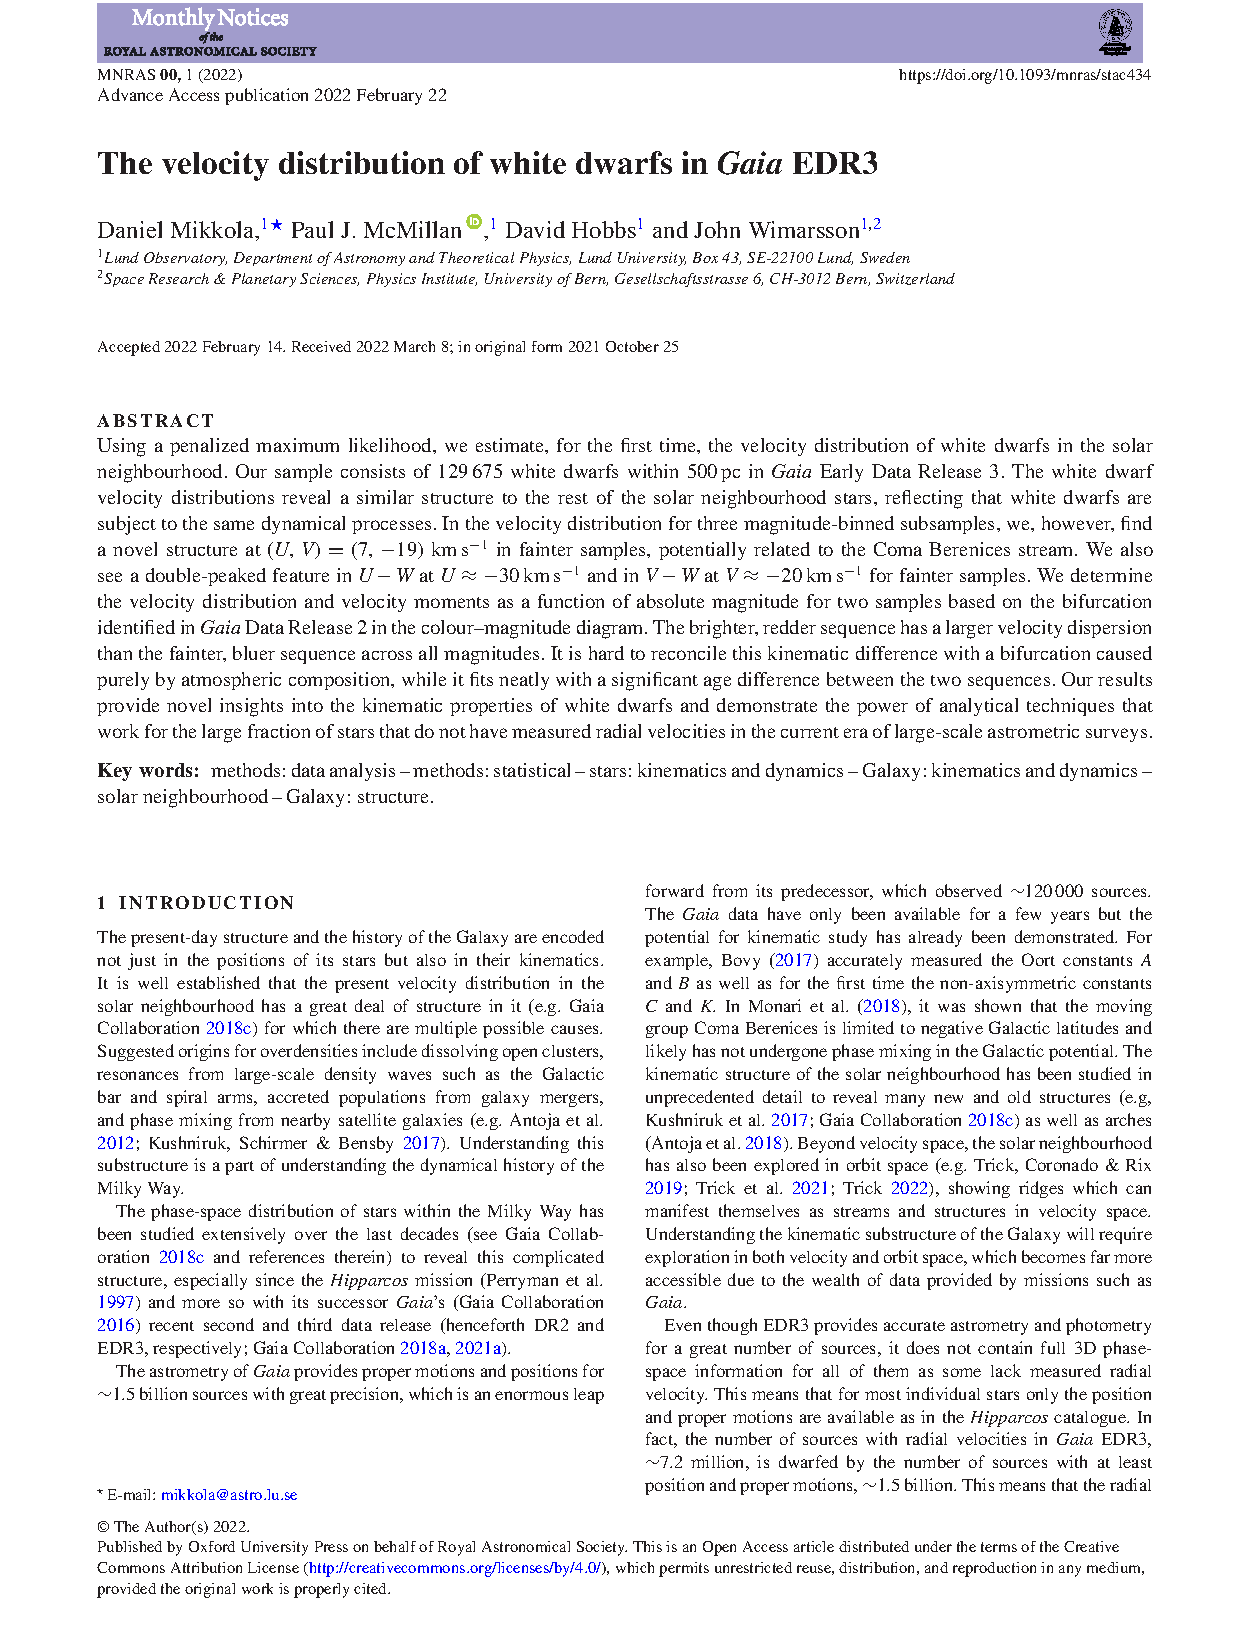
\includepdf[pages=-,width=1.20\textwidth,pagecommand={\thispagestyle{plain}}]{papers/mikkola_2022_whitedwarfs}

% PAPER III
\paperpagemark{The velocity distribution of local halo and disk stars in Gaia DR3 from transverse motion}
\subsection*{Paper III: a titley title}
\textbf{Mikkola, D.}; McMillan, P. J.; Hobbs, D. (to be submitted to MNRAS) \newline

\subsubsection*{My contribution:}
After the second paper, DM and PM had the original idea to expand the method and apply it to other datasets. DM and PM chose two new datasets the largest Solar neighbourhood sample and the stellar halo. PM provided literature sources for velocity distributions of the stellar halo. DM acquired the data and filtered it for quality. DM implemented spherical velocity coordinates into the code and ran the algortithm to produce probability distributions. The analysis in velocities was carried out by DM, with support from PM and DH. PM analysed the data in action space. DM wrote the paper apart from the actions-related section which was written by PM and the paper was reviewed by PM and DH to bring it to a submittable state.
%\includepdf[pages=-,width=1.20\textwidth,pagecommand={\thispagestyle{plain}}]{papers/mikkola_2022_local}



\end{document}
